\documentclass[12pt, a4paper, simple]{eskdtext}

\usepackage{config/main.env}
\usepackage{config/report.env}
\usepackage{styles/listing}
\usepackage{styles/lists}
\usepackage{styles/SectionMargins}
\usepackage{styles/table}
\usepackage{styles/TableOfContent}
\usepackage{styles/url}

\begin{document}
  \begin{ESKDtitlePage}
  \ESKDstyle{empty}
  \begin{center}
    \envReportMinistr \\
    \envReportEducation \\
    \envReportUniversity \\
    \envReportCathedra \\
  \end{center}

  \vfill

  \begin{center}
    Тема: <<\envReportTitle>>
  \end{center}

  \vfill

  \begin{center}
    Отчёт лабораторной работы №\envReportLabNumber \\
    по дисциплине \envReportSubject \\
  \end{center}

  \vfill

  \begin{flushright}
    \begin{minipage}[t]{7cm}
      Выполнил: \\
      \envReportStudentInfo \\
      \hspace{0pt} \\
      Проверил: \\
      \envReportTeacherInfo \\
    \end{minipage}
  \end{flushright}

  \vfill

  \begin{center}
    \envReportCity~\ESKDtheYear
  \end{center}
\end{ESKDtitlePage}


  % = = = = = = = = = = = = = = = =
  \ESKDstyle{empty}
  \begin{center}
    \textbf{Отчёт лабораторной работы №\envReportLabNumber}
  \end{center}

  \paragraph{} \textbf{Тема}: <<\envReportTitle>>

  \paragraph{} \textbf{Цель}:
  Знакомство с Google Cloud Platform, Compute Engine, Cloud SQL, Cloud Logging, Cloud Source Repositories, Endpoints.

  \paragraph{} \textbf{Что нужно сделать}:

  Миграция разработанного в ЛР№1 приложения APP в Google Cloud Platform. Для этого:

  Получите доступ к Google Cloud Platform. Создайте свой первый проект в консоли GCP.
  Ознакомьтесь с описаниями, руководствами на странице \url{https://console.cloud.google.com/getting-started}.
  Подключите биллинг и стандартные API.

  Для контроля версий исходного кода используйте git.
  Создайте новый репозиторий в Cloud Source Repositories и разместите там исходный код своего приложения.

  Создайте экземпляр Compute Engine.
  Проверьте и поймите все параметры конфигурации, в том числе те, которые влияют на стоимость машины.
  Выберите одну из наименьших конфигураций. 

  Настройте SSH-доступ к вновь созданной машине.
  Сначала проверьте доступ через SSH в браузере, потом получите доступ через SSH-соединение
  (через настройку ключей SSH в закладке «Безопасность» виртуальной машины).

  Создайте экземпляр Cloud SQL на базе выбранной вами СУБД.
  Свяжите экземпляр SQL с экземпляром Compute Engine, позволив виртуальной машине связываться с БД на данном экземпляре Cloud SQL.
  Произведите необходимую настройку ВМ для работы с SQL.

  Настройте ВМ (согласно требованиям вашей технологии), не забудьте про git.
  Клонируйте ваше приложение на ВМ и запустите его. Далее будем называть его MS2.

  Настройте агент Fluentd на ВМ для сбора логов и отправки их в Cloud Logging.

  Используйте описание OpenAPI для того, чтобы создать Developer Portal с использованием Endpoints.

  \paragraph{} \textbf{Ход работы}:

  \newpage
  \textbf{Создаем проект}:

  Заходим на сайт Google Cloud Console \cite{GoogleCloudConsole} (см. рисунок~\ref{fig:1}).

  Выбираем проект (там где g.bstu.by, см. рисунок~\ref{fig:1}).

  Жмём <<NEW PROJECT>> (см. рисунок~\ref{fig:1}).

  Project name: \underline{rsiot-po4-190333} (см. рисунок~\ref{fig:2}).

  Жмём <<CREATE>> (см. рисунок~\ref{fig:2}).

  \begin{figure}[!h]
    \centering
    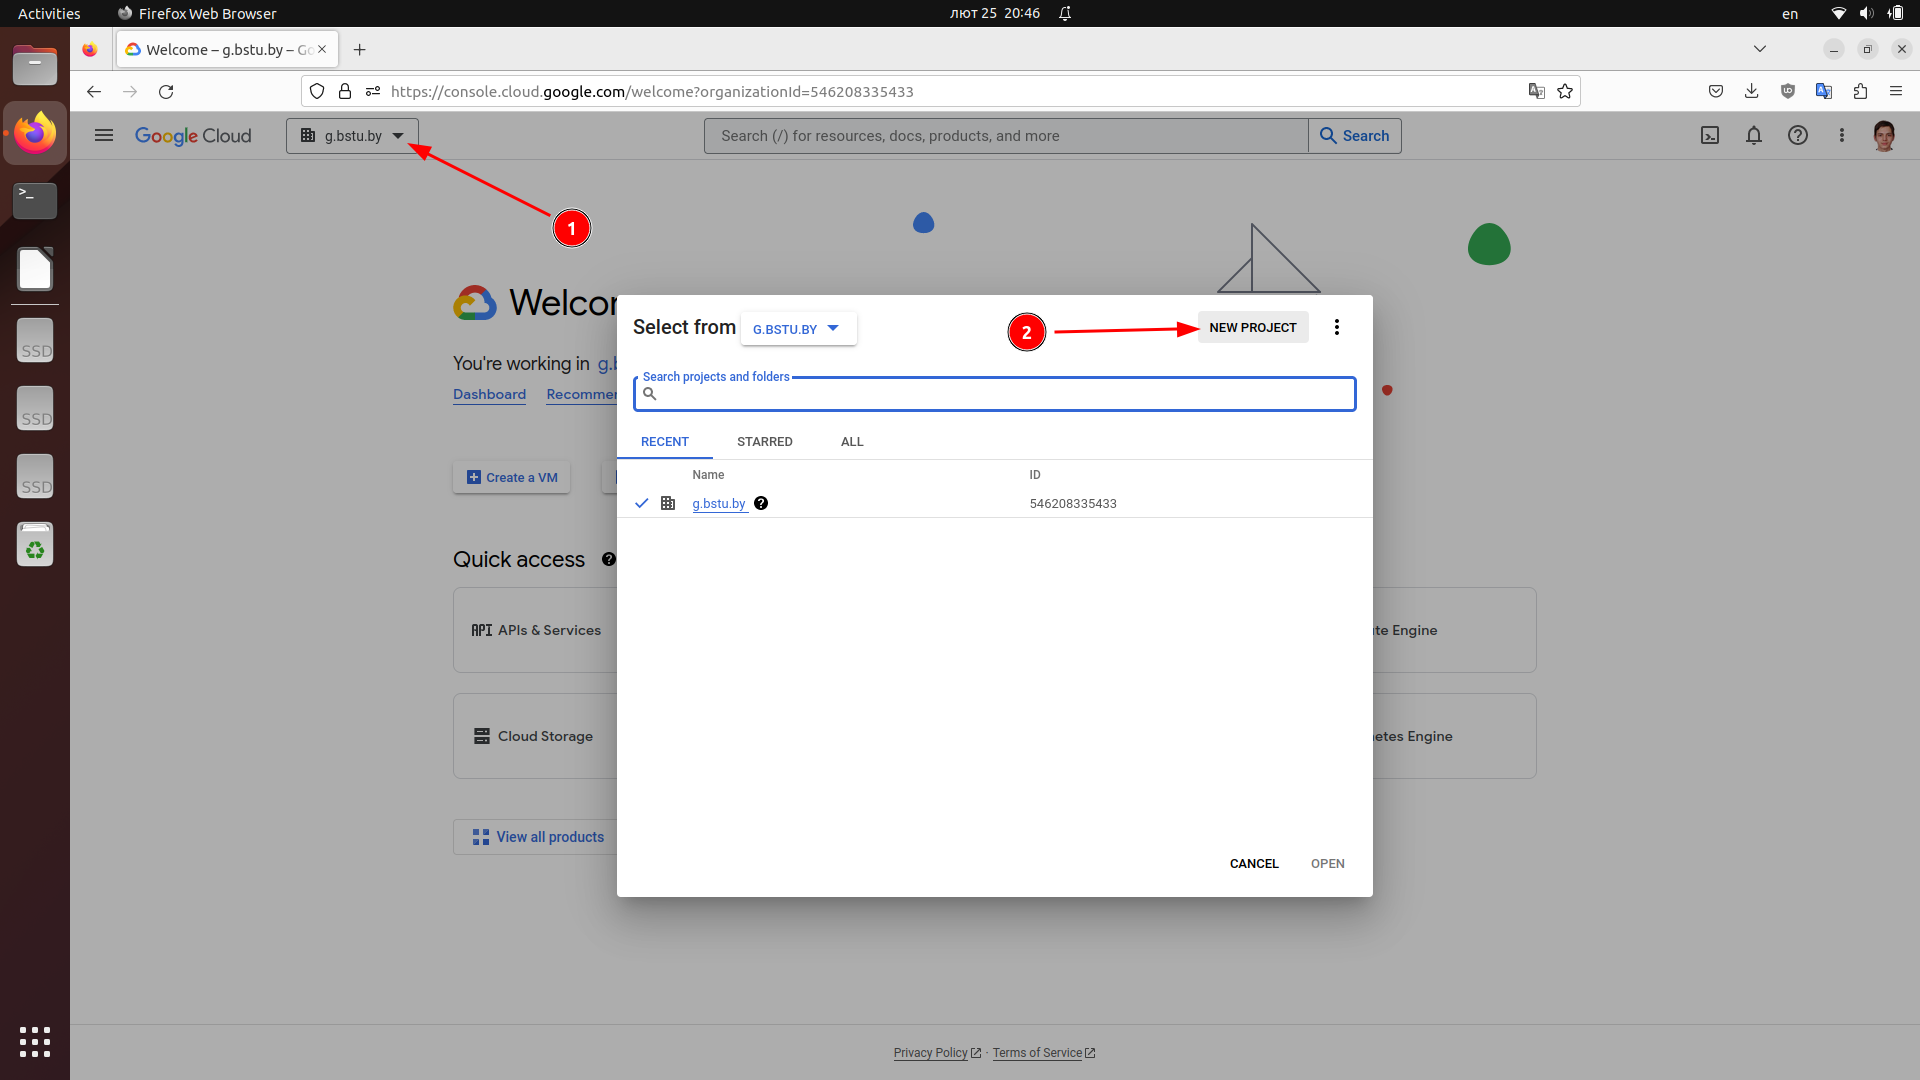
\includegraphics[width=16cm]
    {images/2023-02-25_20-47-00.png}
    \caption{\_}
    \label{fig:1}
  \end{figure}

  \begin{figure}[!h]
    \centering
    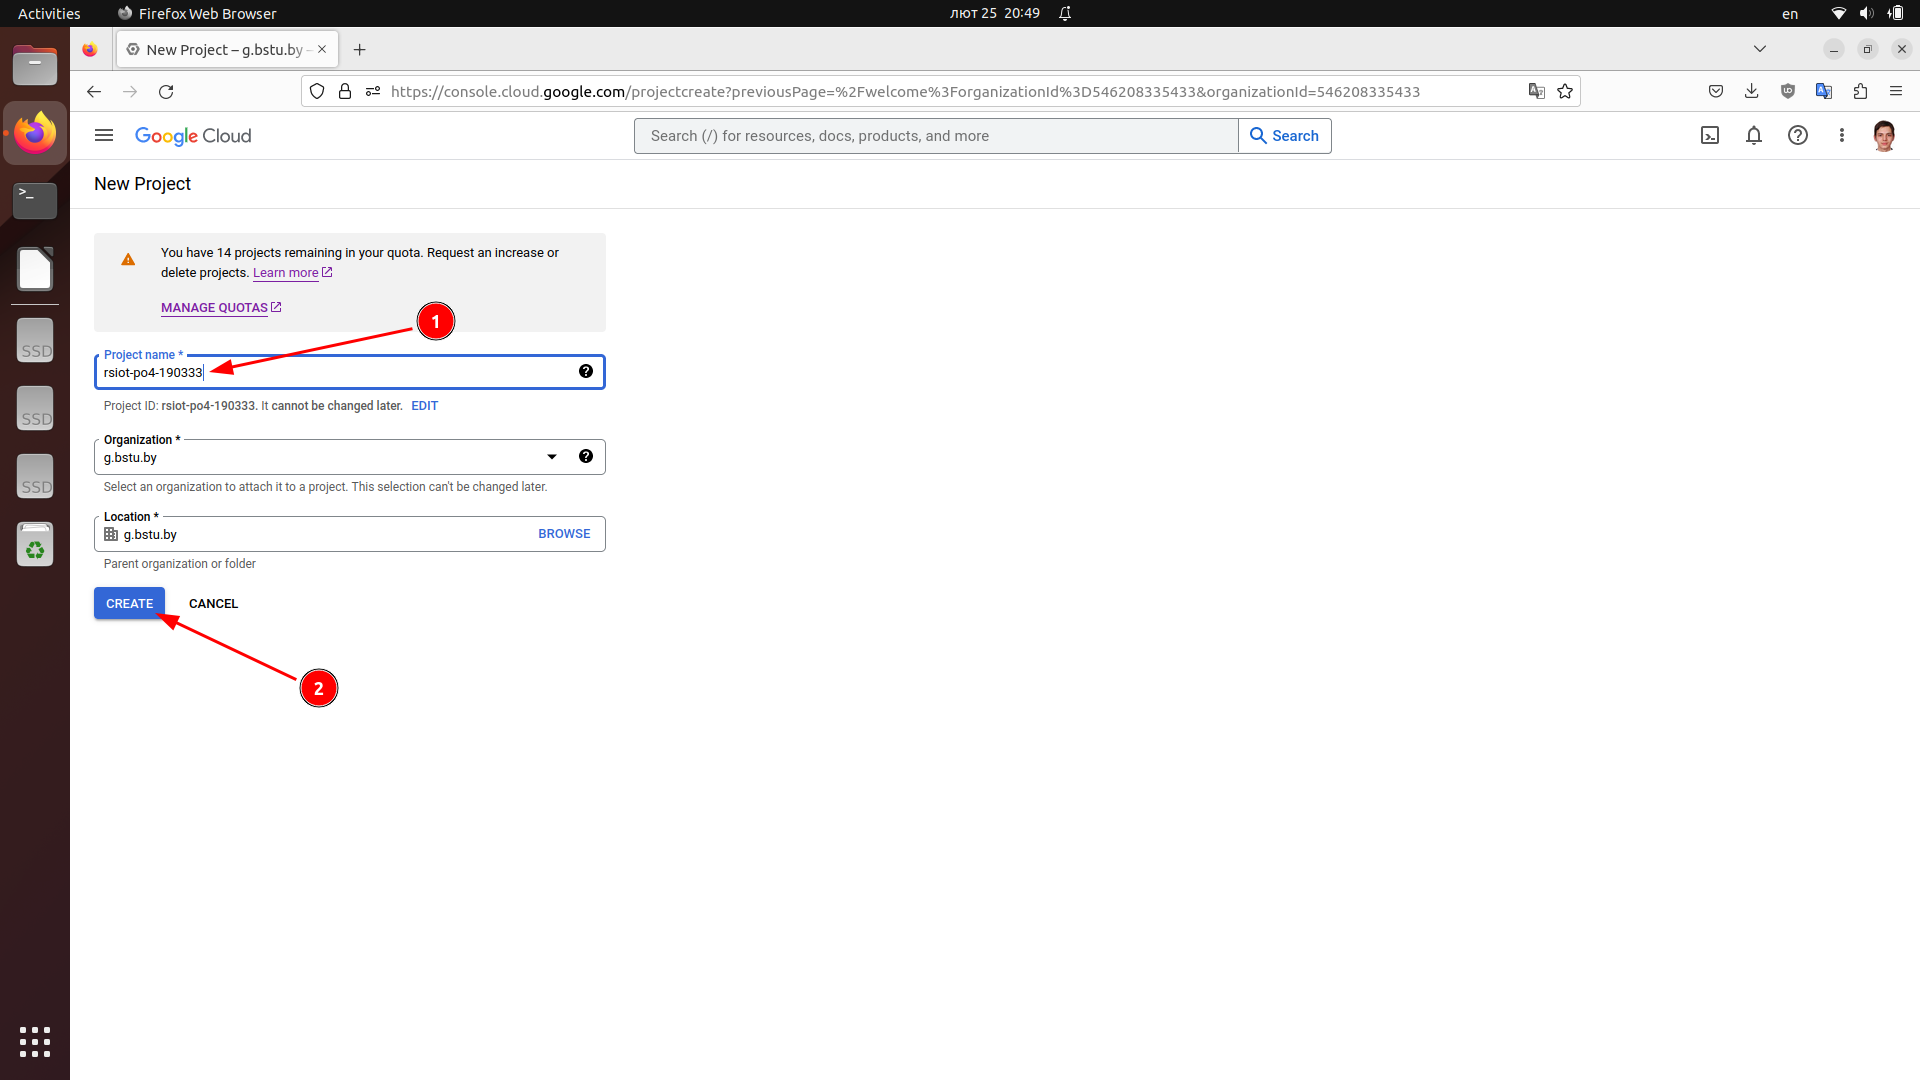
\includegraphics[width=16cm]
    {images/2023-02-25_20-49-58.png}
    \caption{\_}
    \label{fig:2}
  \end{figure}

  \newpage
  \textbf{Создаем Google Cloud Compute Engine}:

  Заходим на сайт Google Cloud Console \cite{GoogleCloudConsole} (см. рисунок~\ref{fig:3}).
  
  Menu > Compute Engine > VM instances

  \begin{figure}[!h]
    \centering
    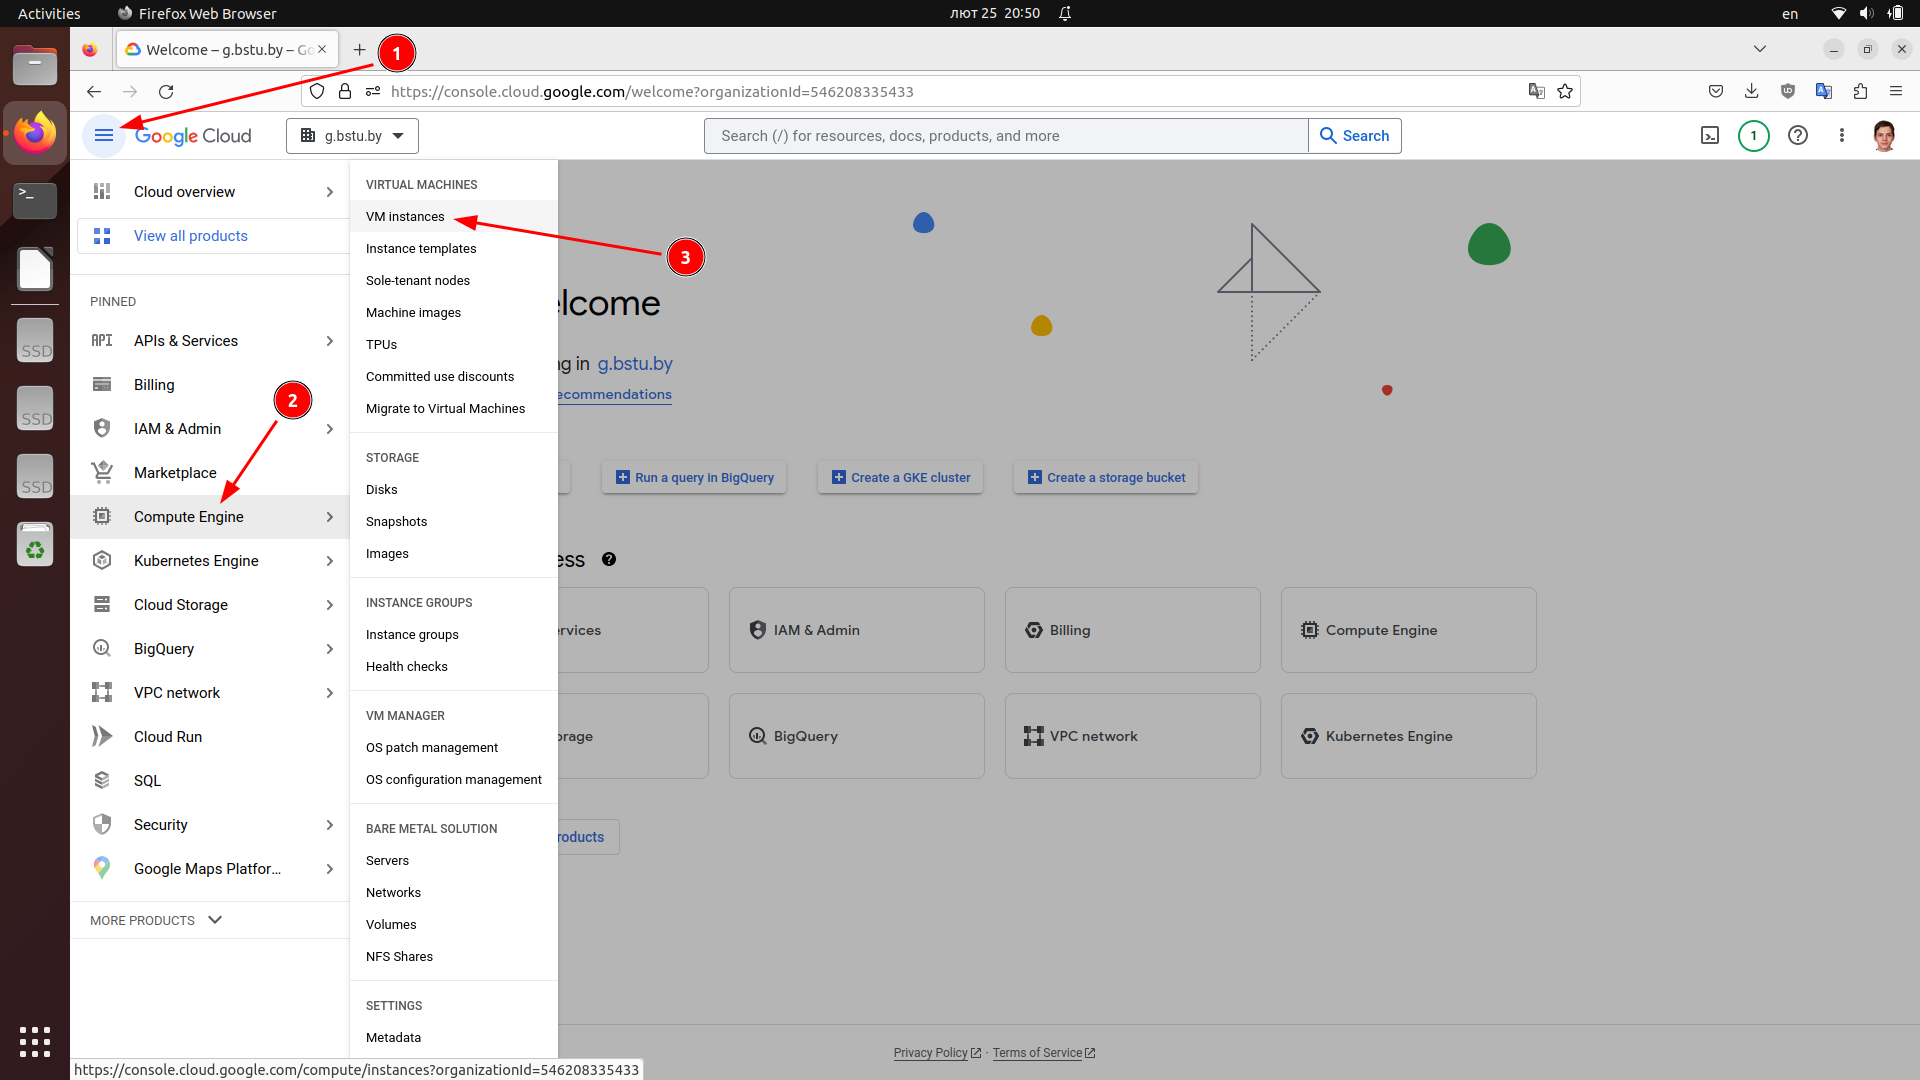
\includegraphics[width=11cm]
    {images/2023-02-25_20-50-57.png}
    \caption{\_}
    \label{fig:3}
  \end{figure}

  Если нужно выбрать проект, то выбираем (см. рисунок~\ref{fig:4}).

  \begin{figure}[!h]
    \centering
    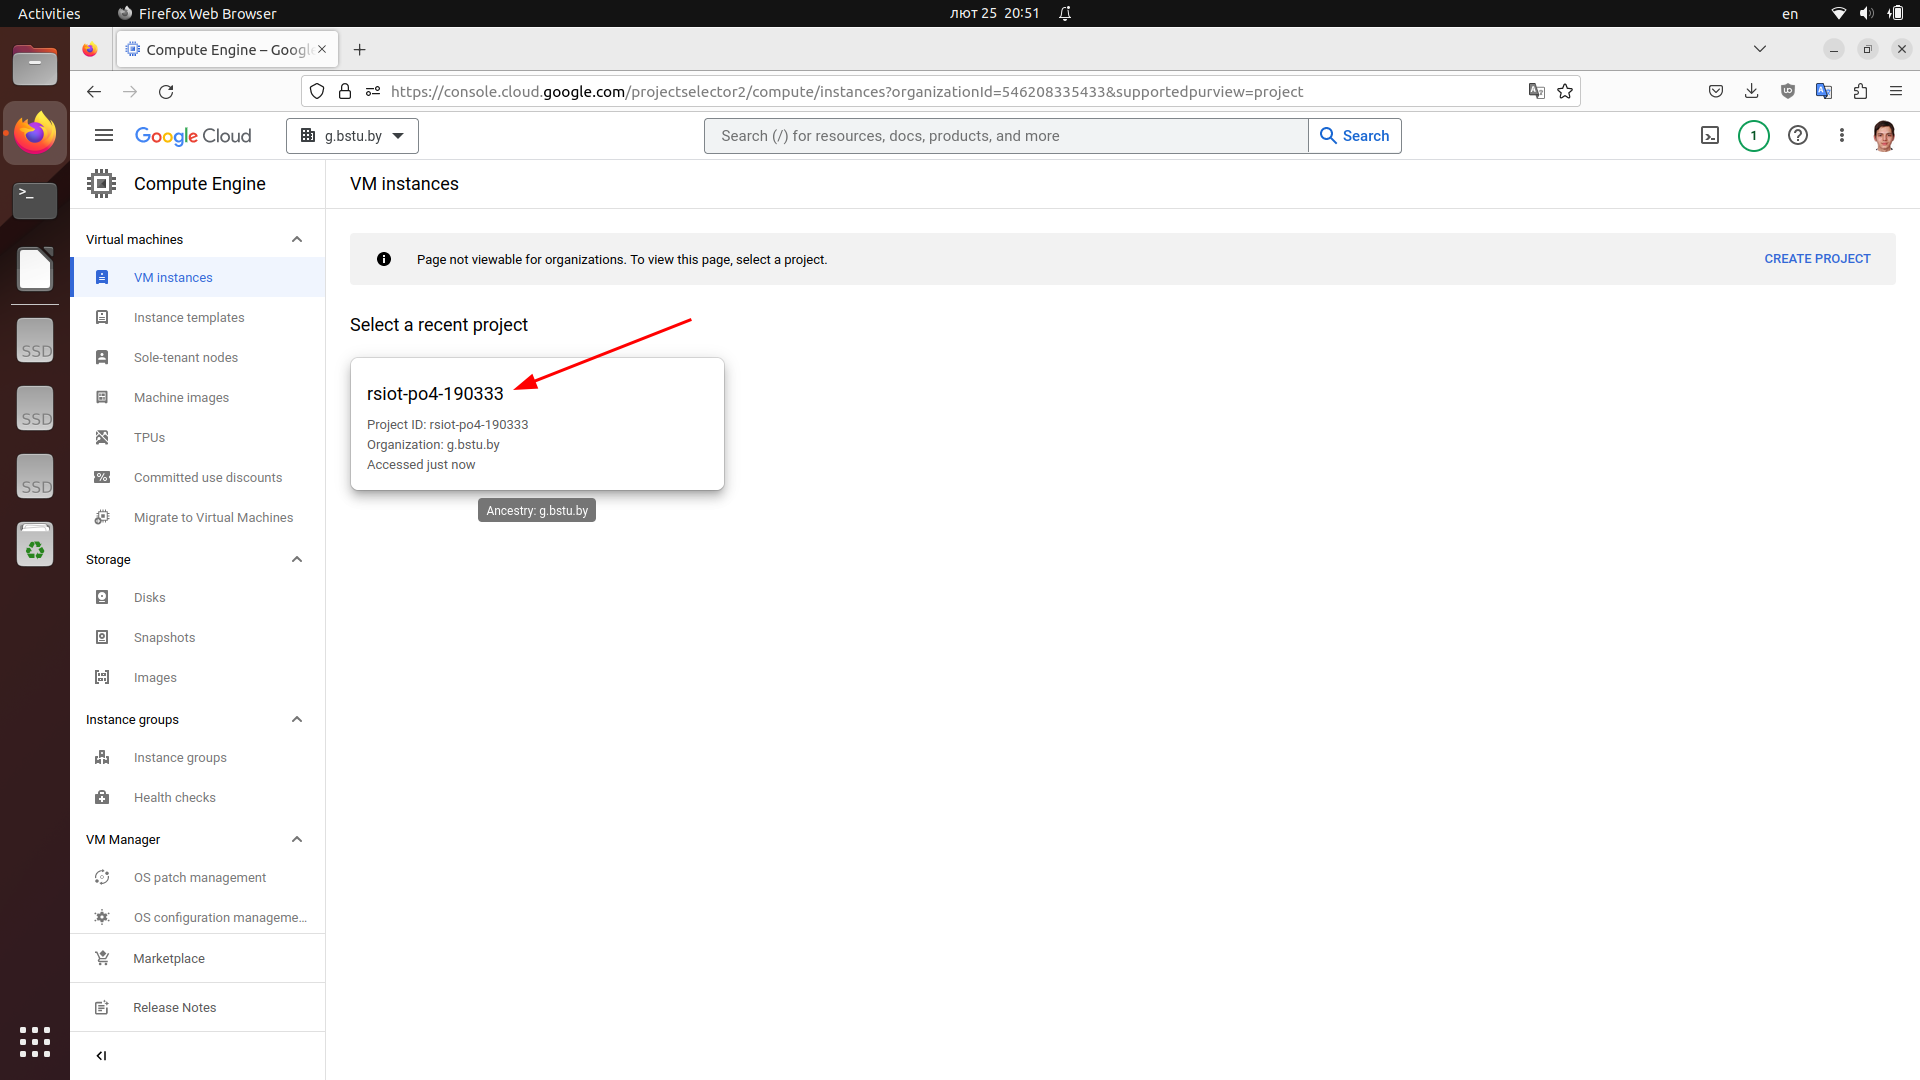
\includegraphics[width=11cm]
    {images/2023-02-25_20-51-20.png}
    \caption{\_}
    \label{fig:4}
  \end{figure}

  Если нужно включить Compute Engine API, то включаем (см. рисунок~\ref{fig:5}).

  \begin{figure}[!h]
    \centering
    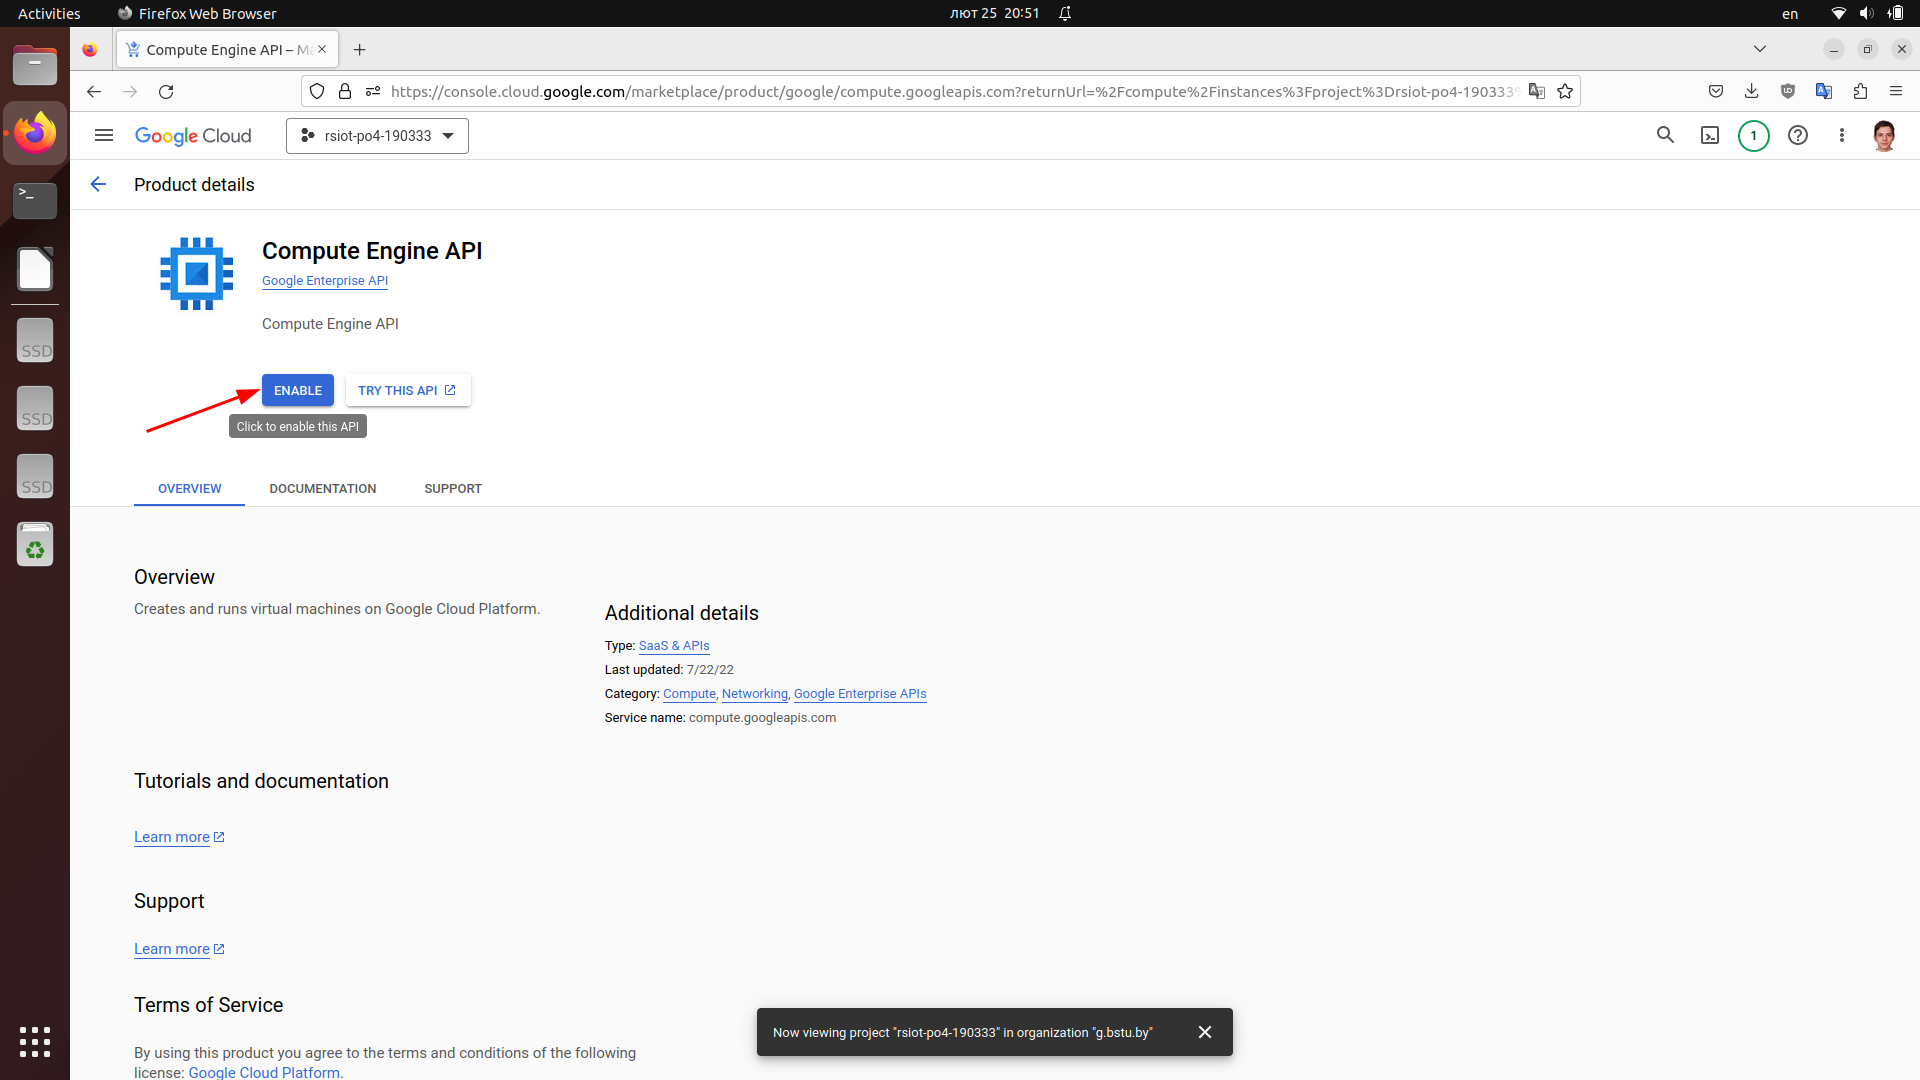
\includegraphics[width=10cm]
    {images/2023-02-25_20-51-41.png}
    \caption{\_}
    \label{fig:5}
  \end{figure}

  \newpage
  Заходим на сайт Google Cloud Compute Engine \cite{GoogleCloudComputeEngine} (см. рисунок~\ref{fig:6}).

  Жму <<CREATE INSTANCE>> (см. рисунок~\ref{fig:6}).

  \begin{figure}[!h]
    \centering
    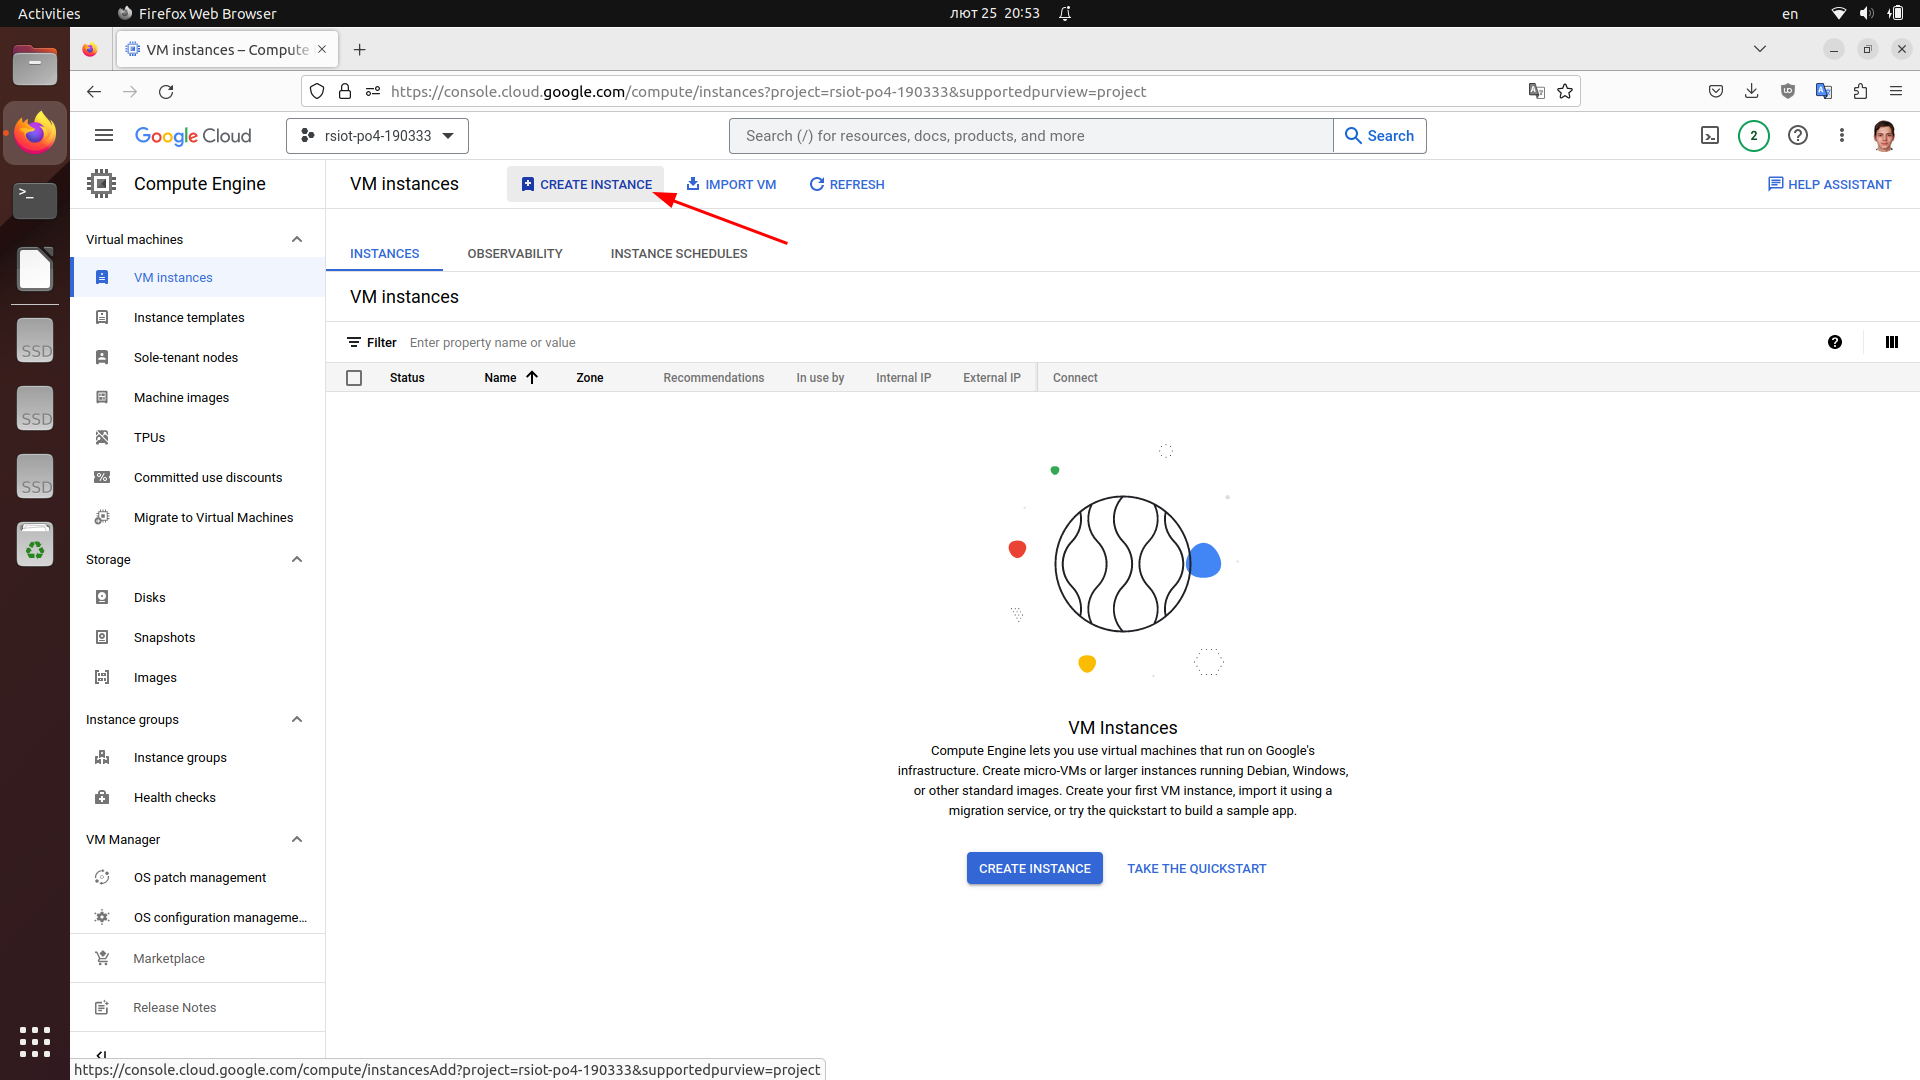
\includegraphics[width=16cm]
    {images/2023-02-25_20-53-33.png}
    \caption{\_}
    \label{fig:6}
  \end{figure}

  Name: \underline{rsiot-po4-190333-compute-engine-instance}.

  Machine type: \underline{e2-micro (2 vCPU 1 GB memory)}.

  Жмём <<СREATE>> (см. рисунок~\ref{fig:7}).

  \begin{figure}[!h]
    \centering
    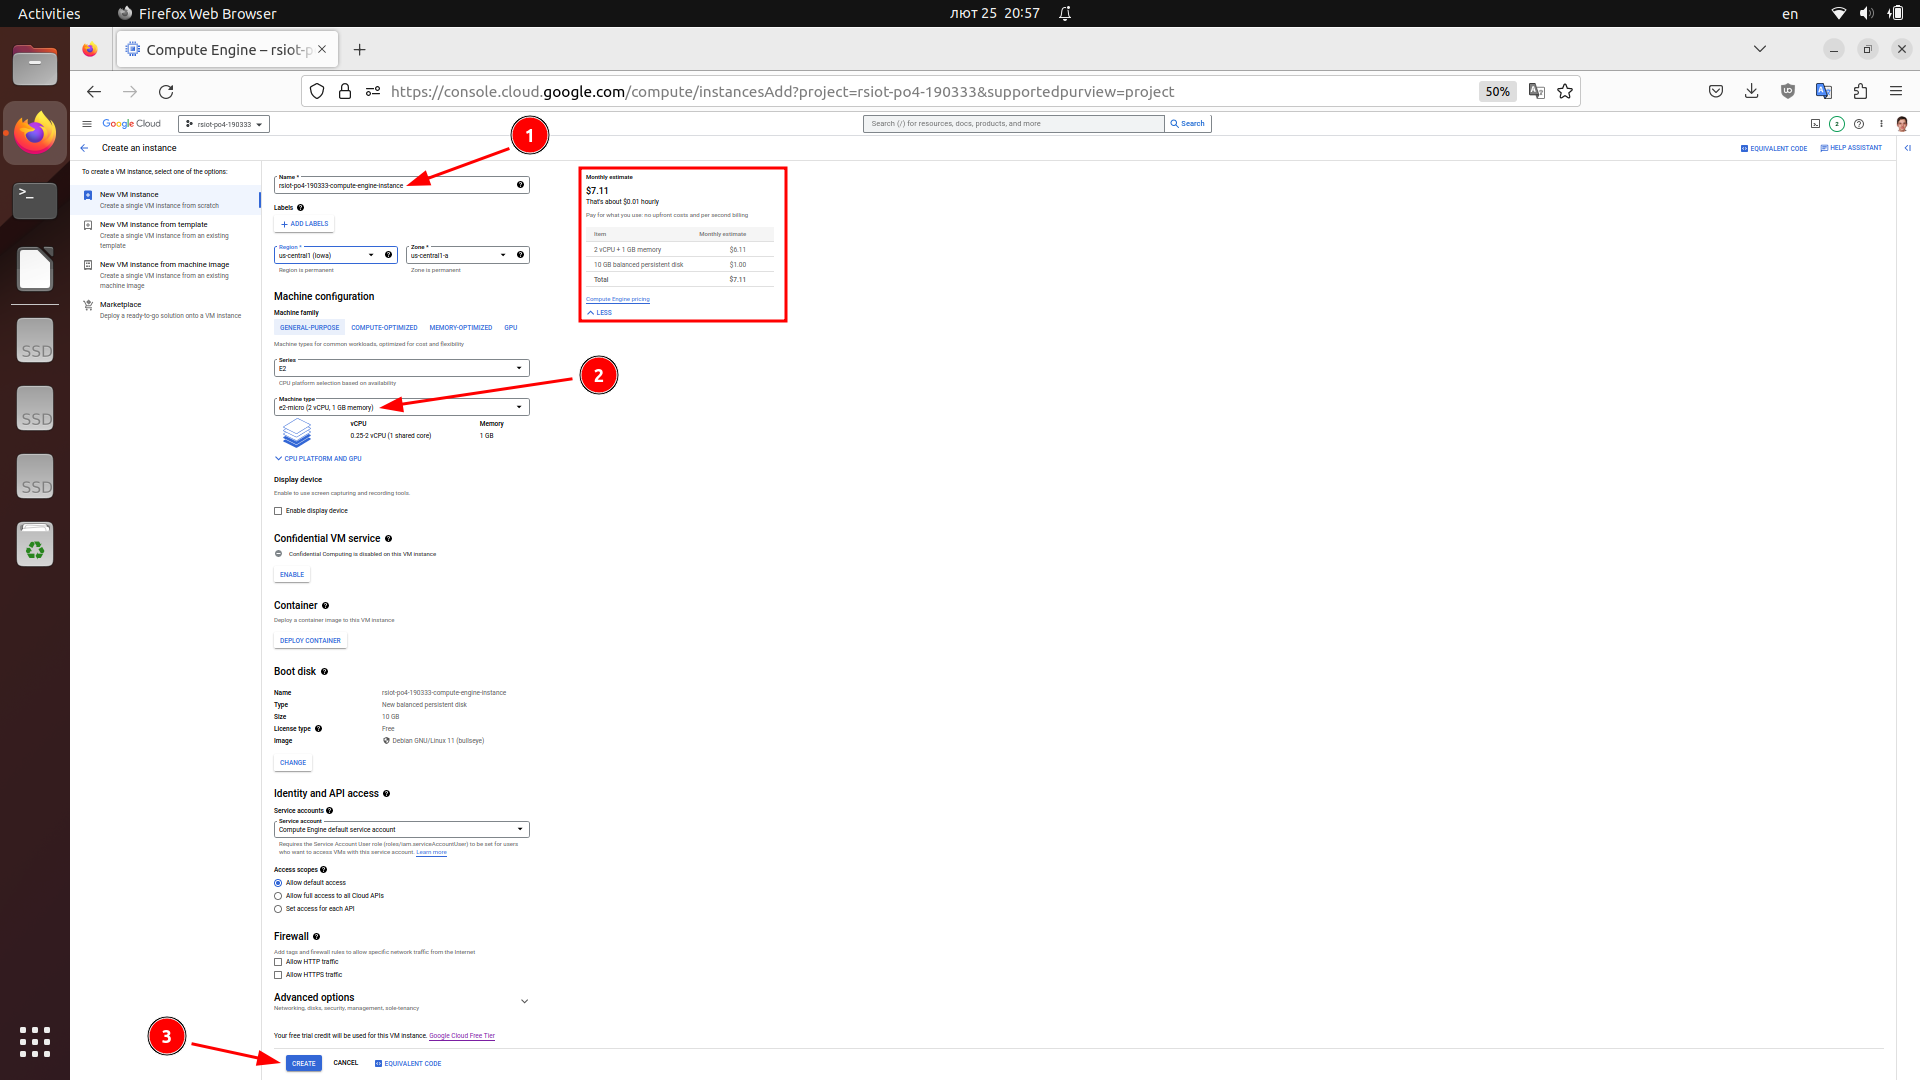
\includegraphics[width=16cm]
    {images/2023-02-25_20-58-22.png}
    \caption{\_}
    \label{fig:7}
  \end{figure}

  \newpage
  \textbf{SSH-подключение через браузере}

  Заходим на сайт Google Cloud Compute Engine \cite{GoogleCloudComputeEngine} (см. рисунок~\ref{fig:8}).

  Жмём <<SSH>> (см. рисунок~\ref{fig:8}).

  \begin{figure}[!h]
    \centering
    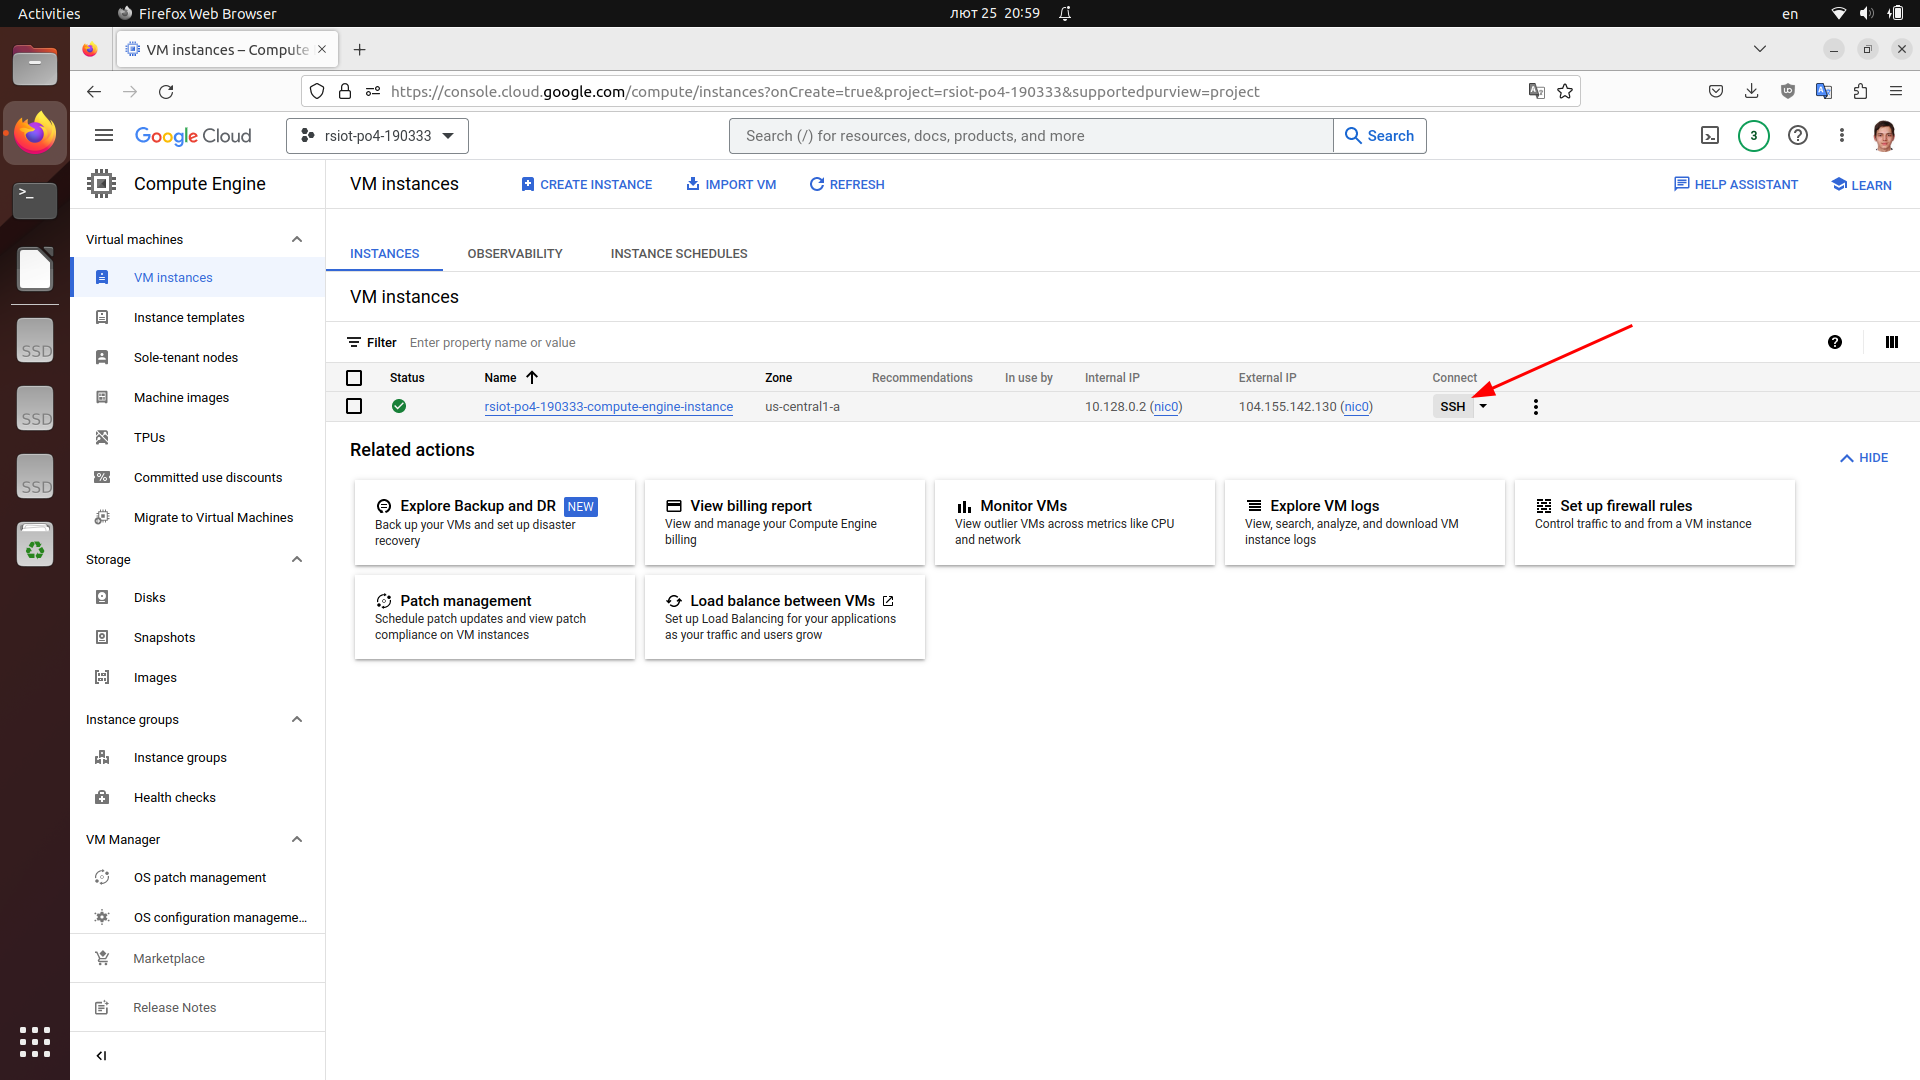
\includegraphics[width=16cm]
    {images/2023-02-25_20-59-45.png}
    \caption{\_}
    \label{fig:8}
  \end{figure}

  Открылось новое окно в браузере (см. рисунок~\ref{fig:9}). Теперь можем устанавливать программы как в Linux Ubuntu через apt.

  \begin{figure}[!h]
    \centering
    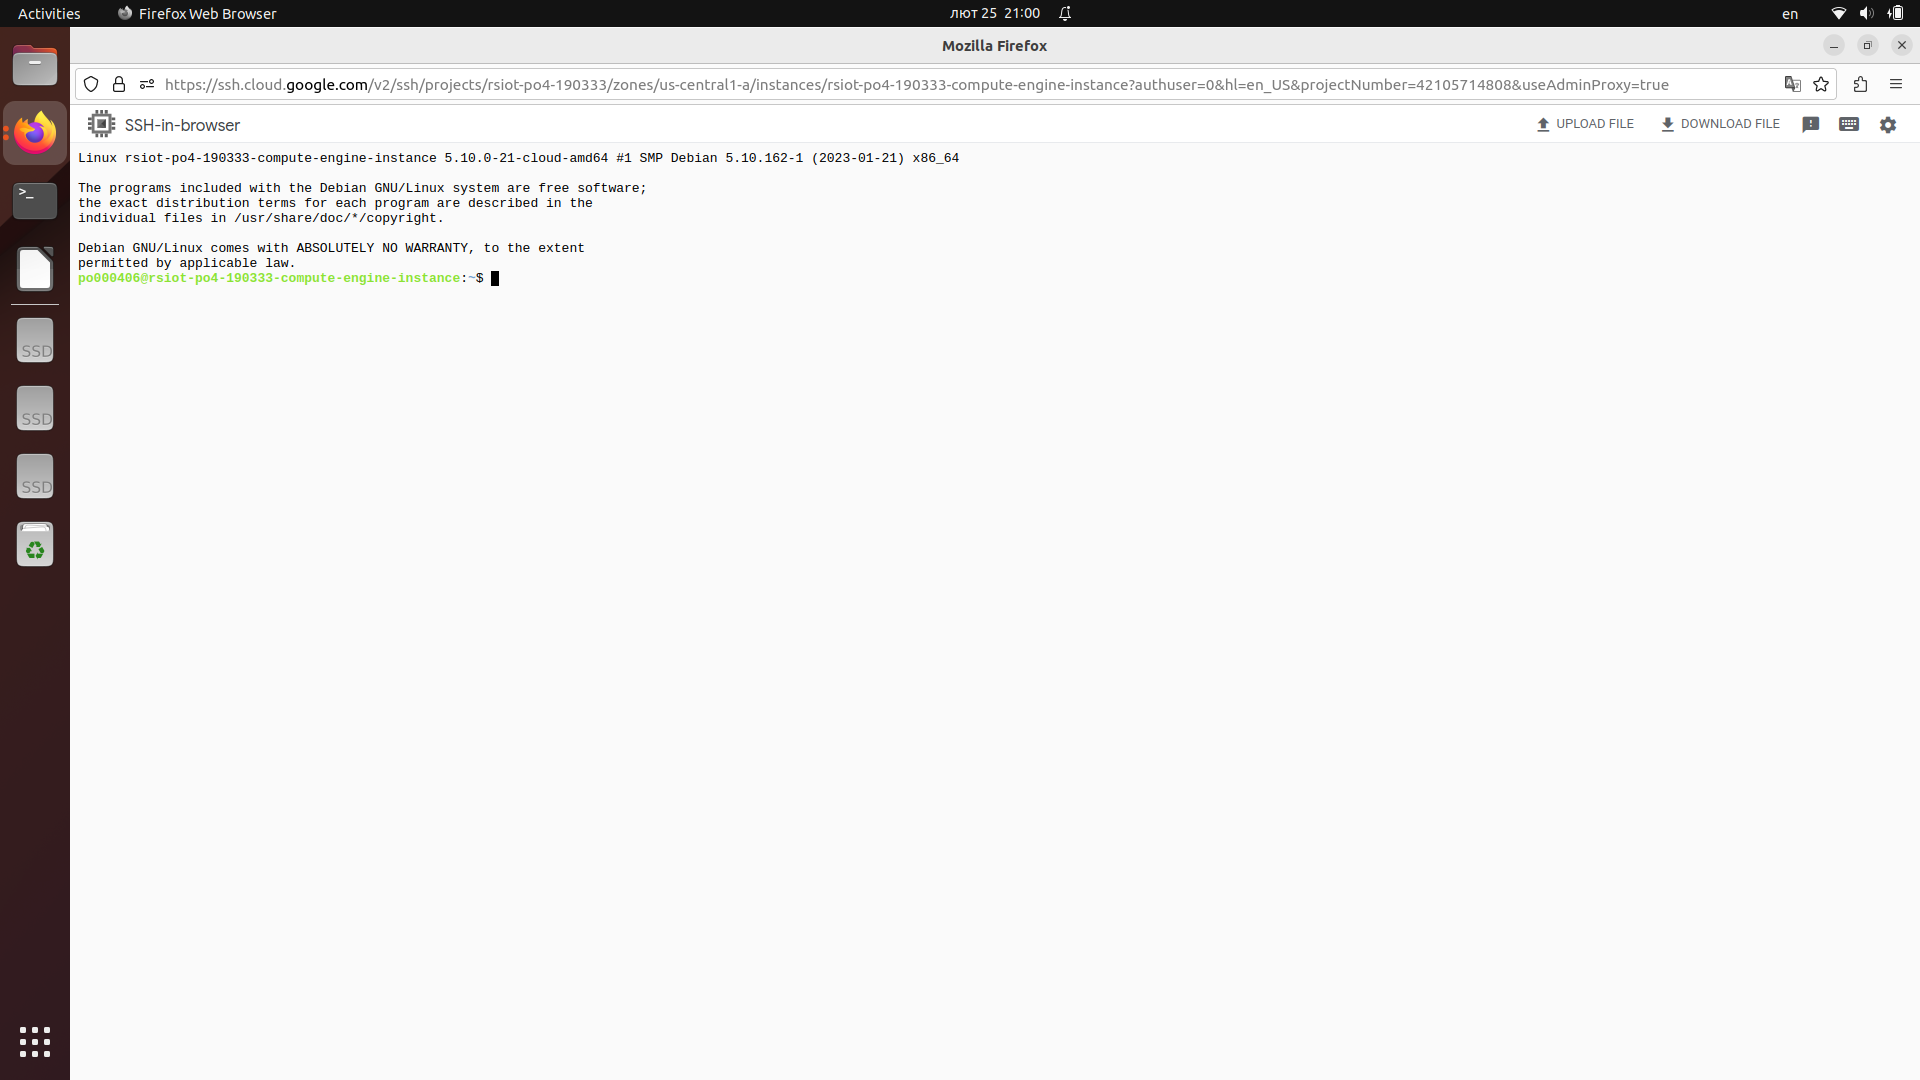
\includegraphics[width=16cm]
    {images/2023-02-25_21-00-38.png}
    \caption{\_}
    \label{fig:9}
  \end{figure}

  \newpage
  \textbf{SSH-подключение через свой ноутбук}

  Заходим на сайт Google Cloud Compute Engine \cite{GoogleCloudComputeEngine} (см. рисунок~\ref{fig:10}).

  Жмём по имени: \underline{rsiot-po4-190333-compute-engine-instances} (см. рисунок~\ref{fig:10}).

  \begin{figure}[!h]
    \centering
    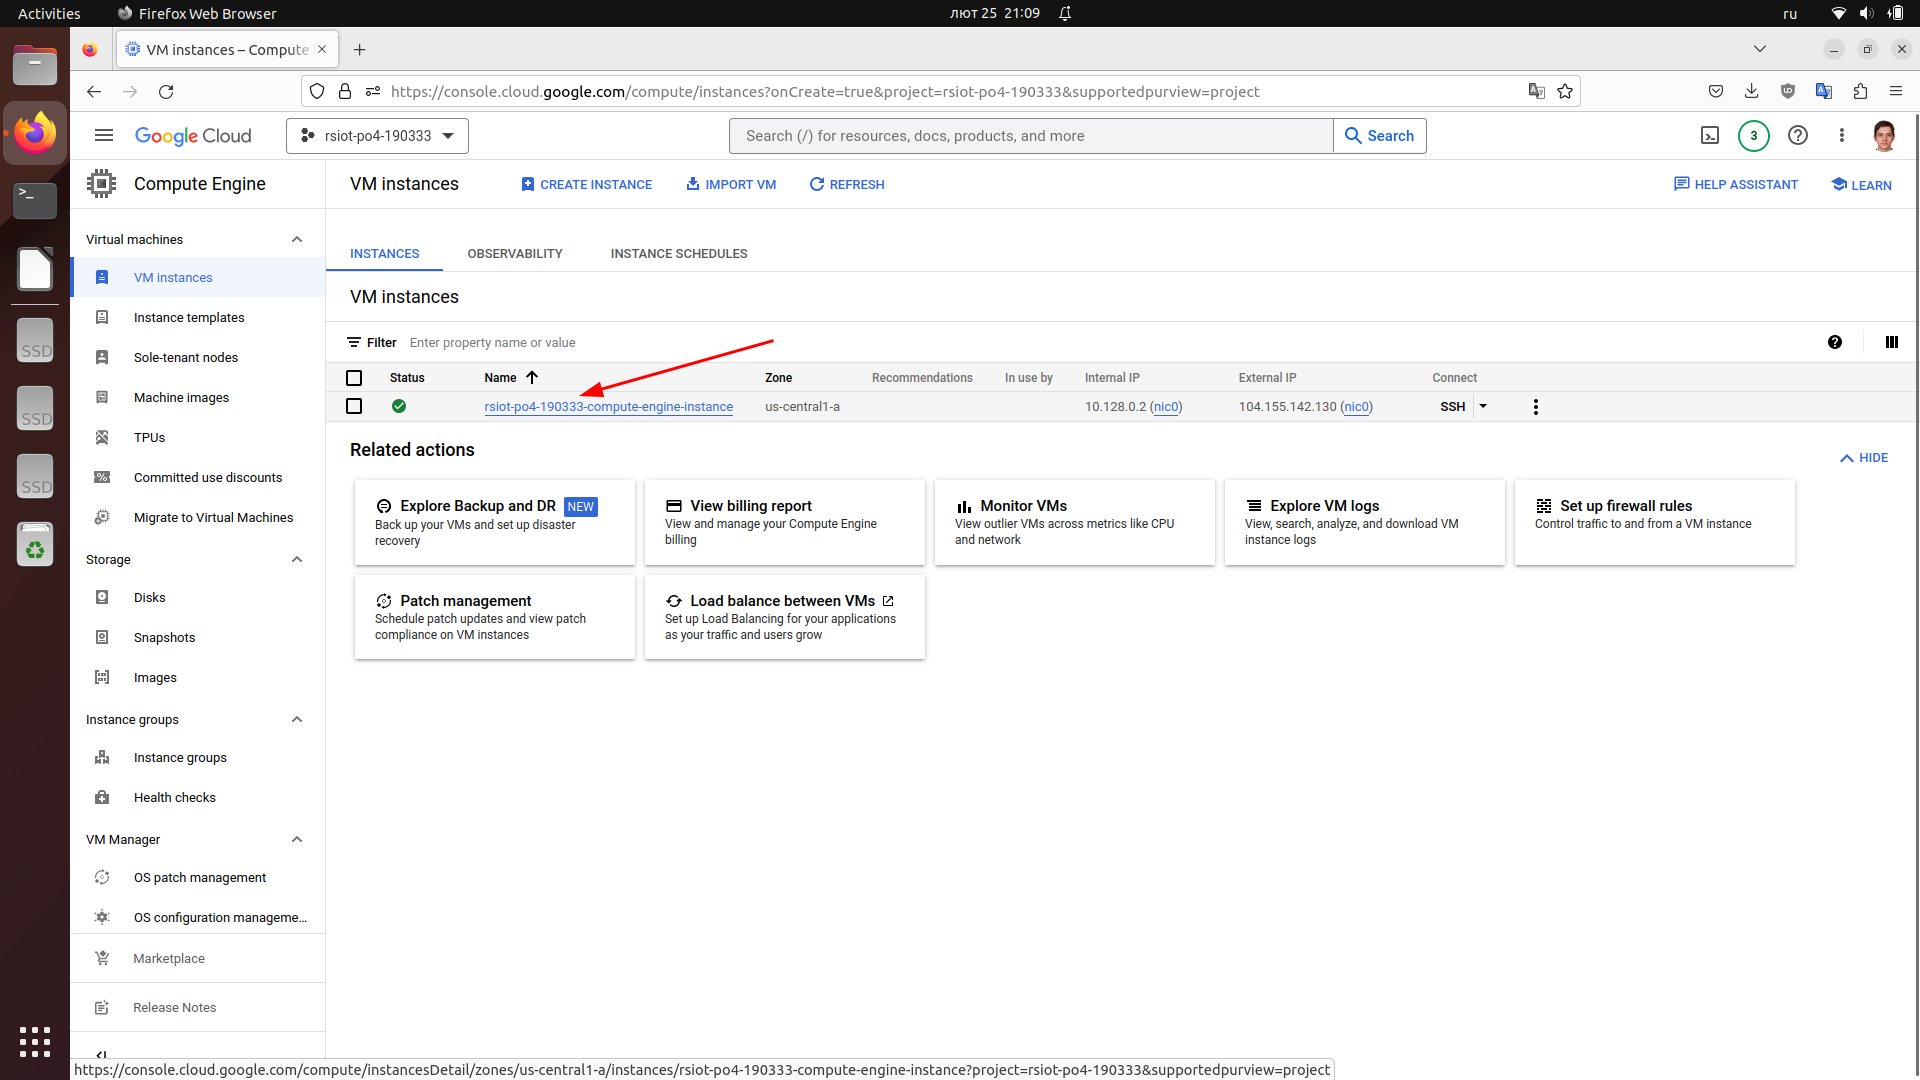
\includegraphics[width=16cm]
    {images/2023-02-25_21-09-26.png}
    \caption{\_}
    \label{fig:10}
  \end{figure}

  Жмём <<EDIT>> (см. рисунок~\ref{fig:11}).

  \begin{figure}[!h]
    \centering
    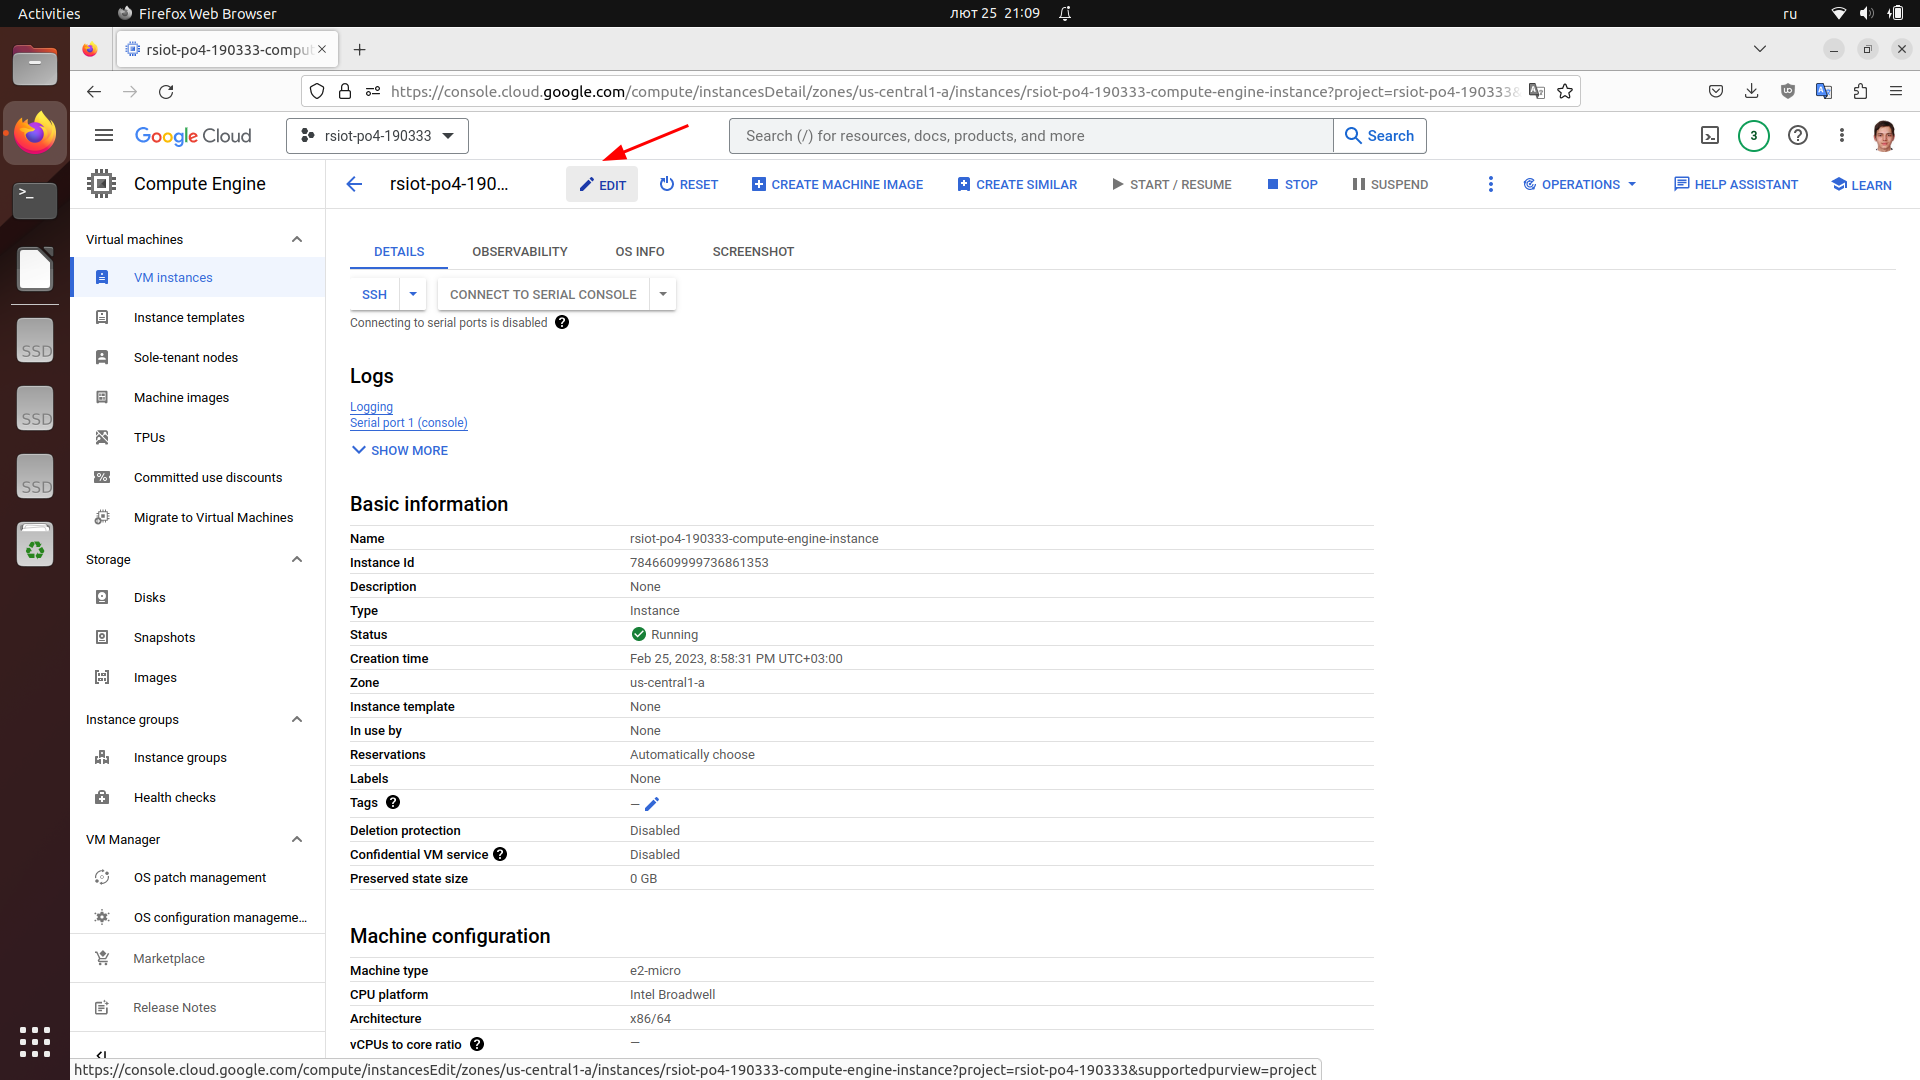
\includegraphics[width=12cm]
    {images/2023-02-25_21-09-46.png}
    \caption{\_}
    \label{fig:11}
  \end{figure}

  Там где <<SSH Keys>> жмём <<ADD ITEM>> (см. рисунок~\ref{fig:12}).
  
  Открываю терминал.

  Пишу в терминале <<ssh-keygen>>.

  Файл: \underline{/home/ph/.ssh/rsiot-po4-190333-compute-engine-instance}.

  Фраза: \underline{secret}.

  Повторяем фразу: \underline{secret}.

  Выводим публичный ключ в терминал: <<cat /home/ph/.ssh/rsiot-po4-190333-compute-engine-instance>>.

  Копируем публичный ключ.

  Вставляем публичный ключ в яцейку на сайте (см. рисунок~\ref{fig:12}).

  Жму <<SAVE>> (см. рисунок~\ref{fig:12}).

  \begin{figure}[!h]
    \centering
    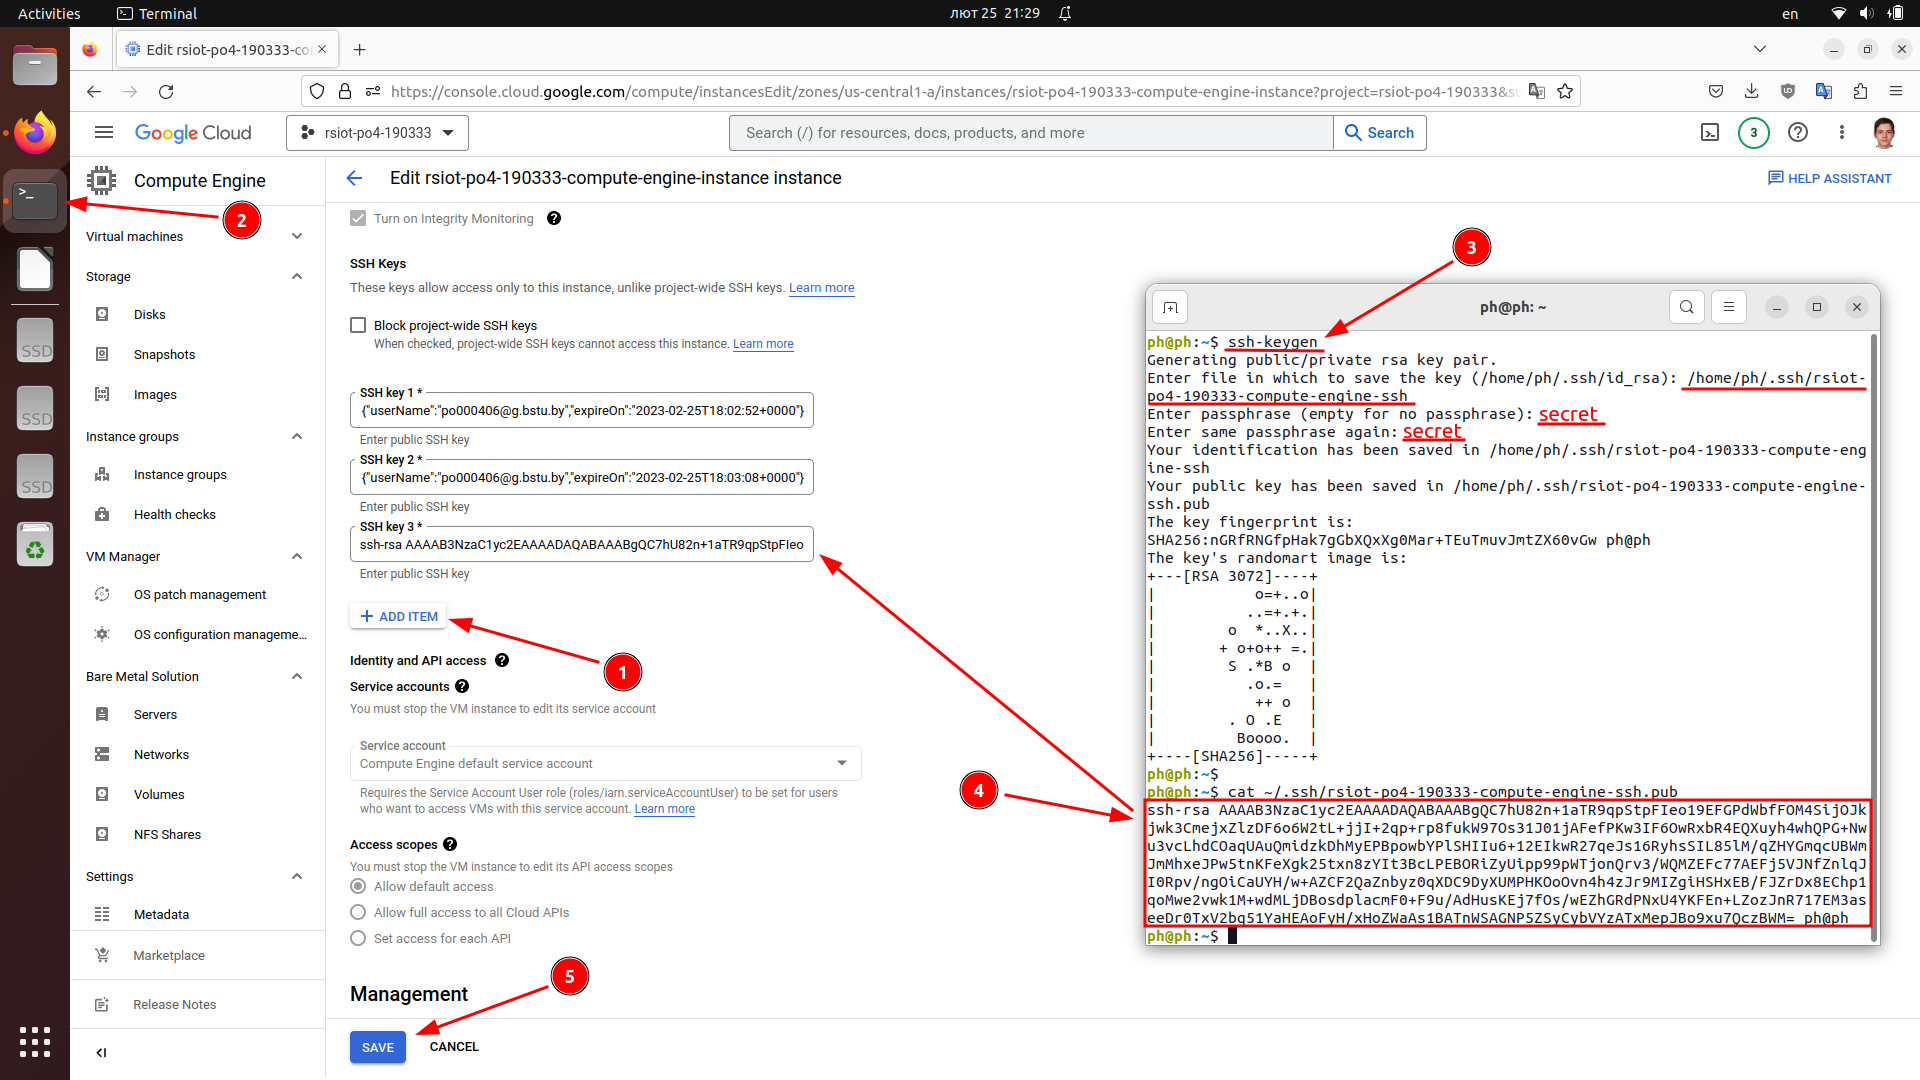
\includegraphics[width=18cm]
    {images/2023-02-25_21-32-41.png}
    \caption{\_}
    \label{fig:12}
  \end{figure}

  Открываем терминал (см. рисунок~\ref{fig:13}).

  Подключаемся <<ssh external-ip-compute-engine>> (см. рисунок~\ref{fig:13}).

  \begin{figure}[!h]
    \centering
  
    \begin{minipage}{0.49\textwidth}
      \centering
  
      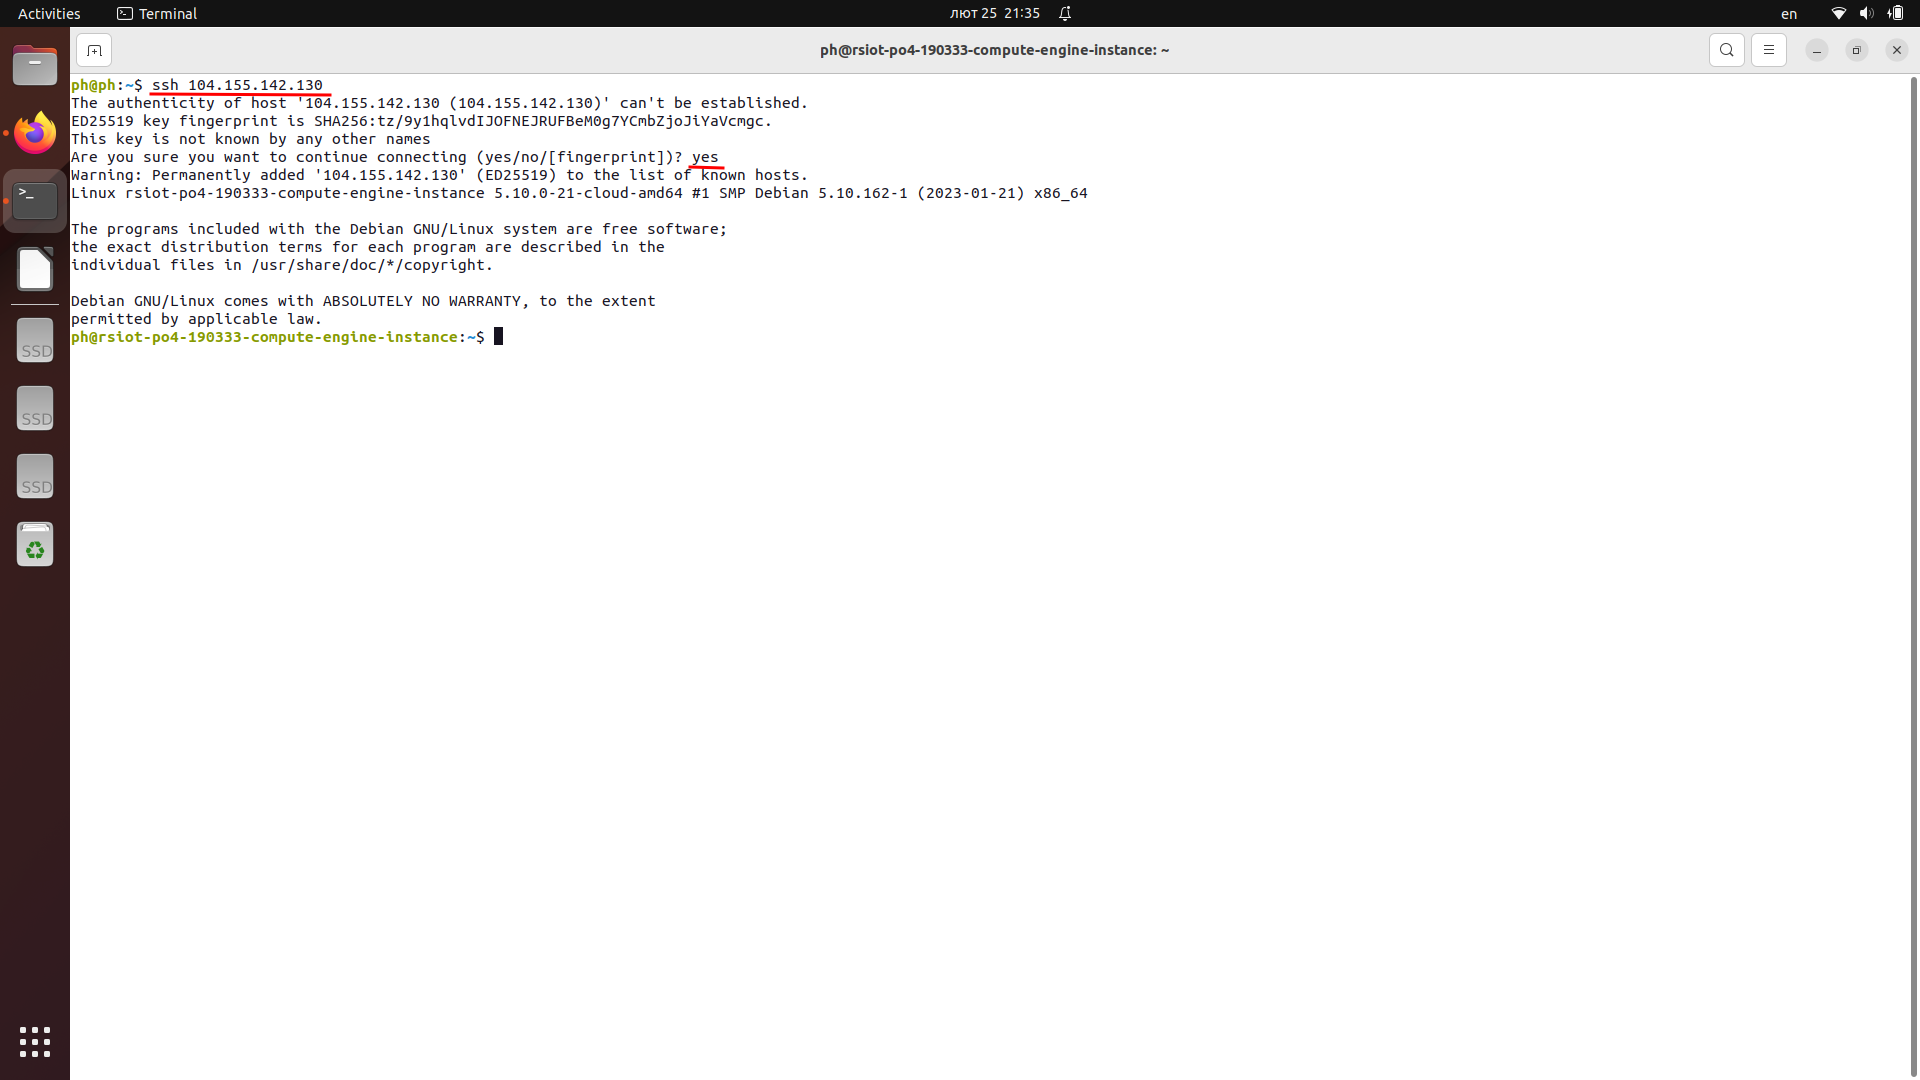
\includegraphics[height=5cm]
      {images/2023-02-25_21-36-15.png}
  
      \caption{\_}
  
      \label{fig:13}
    \end{minipage}
    \begin{minipage}{0.49\textwidth}
      \centering
  
      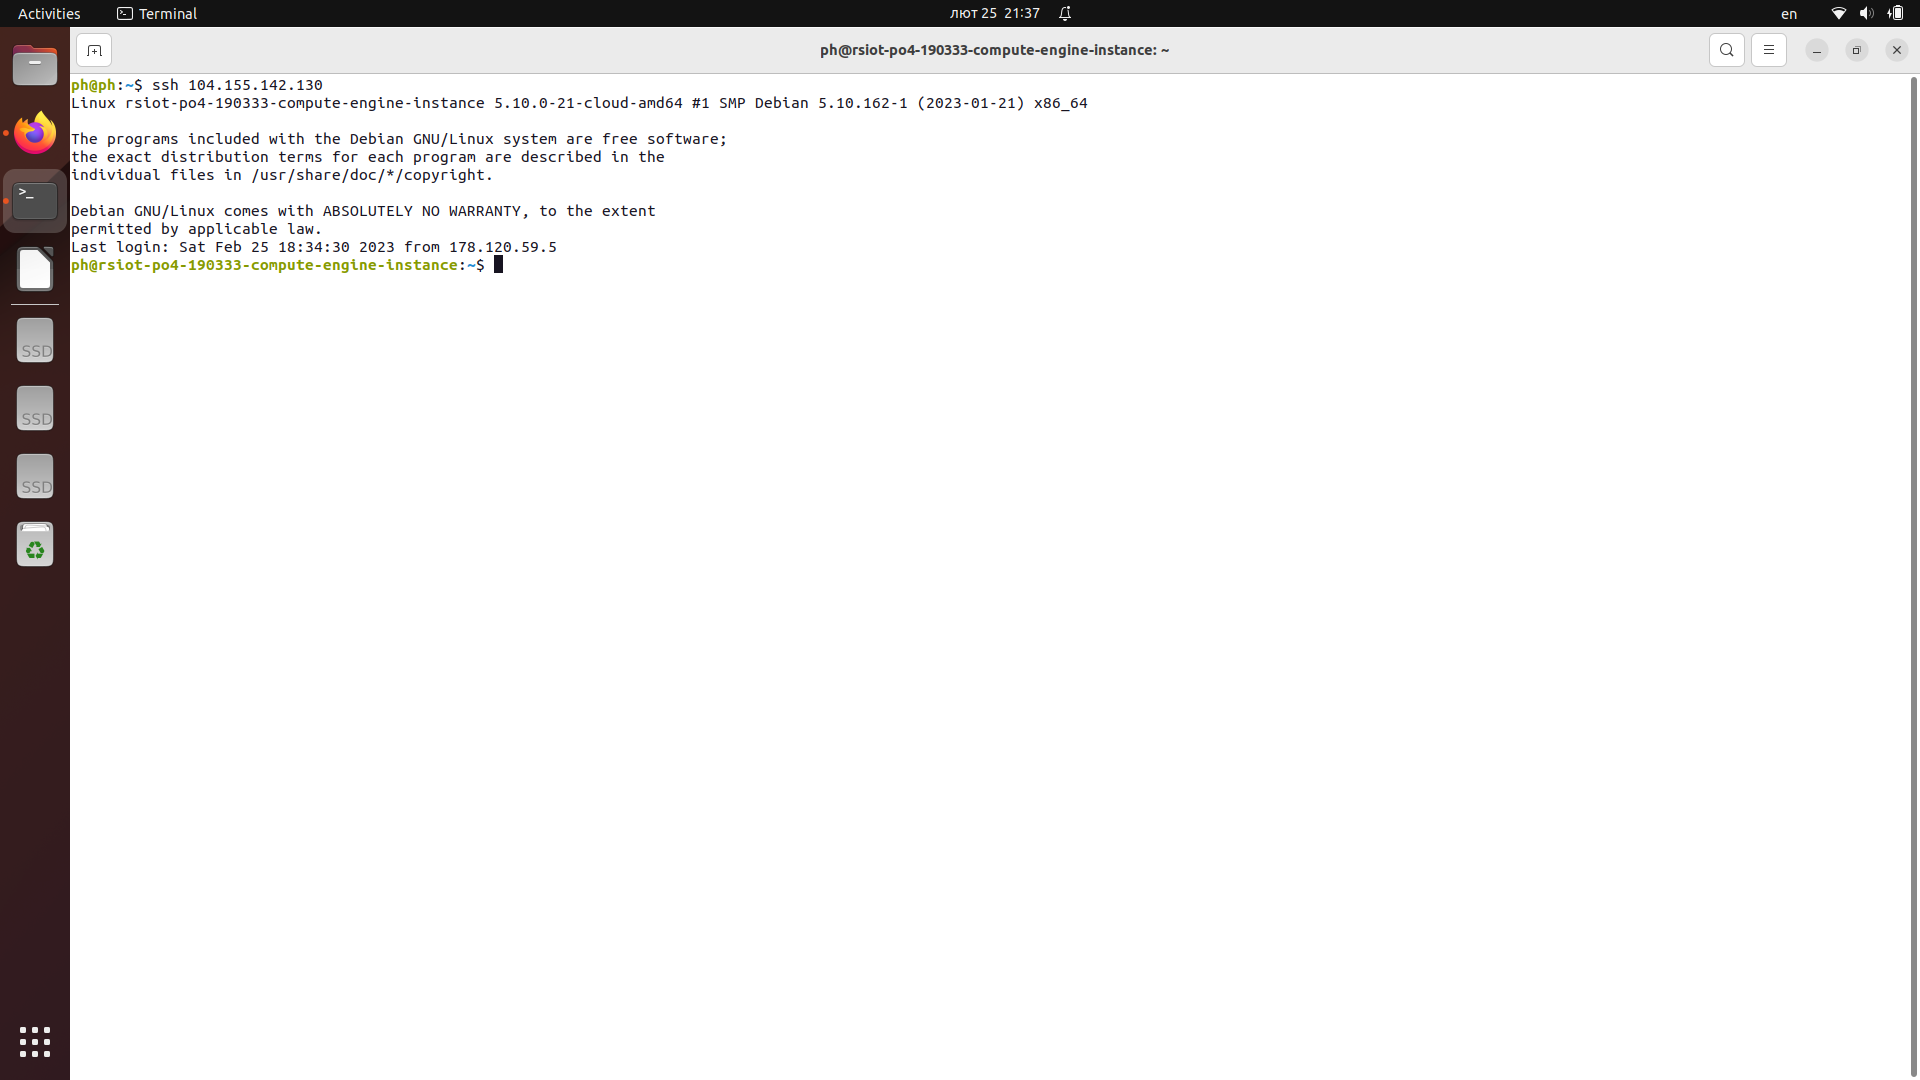
\includegraphics[height=5cm]
      {images/2023-02-25_21-37-30.png}
  
      \caption{\_}
  
      \label{fig:14}
    \end{minipage}
  \end{figure}

  \newpage

  \begin{lstlisting}[language=bash,name=Установка Git]
    sudo apt update
    sudo apt install git
  \end{lstlisting}

  \begin{lstlisting}[language=bash,name=Установка NodeJS и yarn]
    sudo apt update
    sudo apt install curl
    curl -fsSL https://deb.nodesource.com/setup_lts.x | sudo -E bash
    sudo apt-get install -y nodejs

    npm i -g yarn
  \end{lstlisting}

  \begin{lstlisting}[language=bash,name=Установка Docker и docker-compose]
    sudo apt update
    sudo apt install docker.io
    sudo apt install docker-compose
    
    sudo groupadd docker
    sudo gpasswd -a $USER docker
    newgrp docker
  \end{lstlisting}

  \begin{lstlisting}[language=bash,name=Установка make (для Makefile)]
    sudo apt update
    sudo apt install make
  \end{lstlisting}

  \begin{lstlisting}[language=bash,name=Установка консольного файлового менеджера mc]
    sudo apt update
    sudo apt install mc
  \end{lstlisting}

  \begin{lstlisting}[language=bash,name=Установка консольного диспетчера задач htop]
    sudo apt update
    sudo apt install htop
  \end{lstlisting}

  \begin{lstlisting}[language=bash,name=Клонирования репозитория]
    ssh-keygen # Enter, Enter, Enter
    cat ~/.ssh/id_rsa.pub # Copy and paste to https://github.com/settings/ssh/new
    git clone git@github.com:BrSTU-PO4-190333/8sem_RSiOT.git
    cd 8sem_RSiOT/lab1/sources/APP
    yarn # npm i
  \end{lstlisting}

  \begin{lstlisting}[language=bash,name=Запуск режима dev]
    cp dev.env.example dev.env
    make dev-d  # Старт Postgres из docker-compose
    make dev    # Старт NestJS (запустятся сборка, затем миграции, затем приложение)
    # если APP_PORT=80, то через sudo: $ sudo make dev
  \end{lstlisting}

  \begin{lstlisting}[name=dev.env для c БД в docker-compose]
    APP_PORT=80

    DMS_HOST=localhost
    DMS_PORT=25432
    DMS_USER=admin
    DMS_PASS=secret123password
    DMS_NAME=database

    OUT_PORT_DTB=25432
    OUT_PORT_ADM=28080
  \end{lstlisting}

  \begin{lstlisting}[language=bash,name=Установка Postresql]
    sudo apt update
    sudo apt install postgresql
    sudo -i -u postgres
  
    CREATE DATABASE database;
    CREATE USER admin;
    ALTER USER admin password 'secret123password';
    exit
    exit
  \end{lstlisting}

  \begin{lstlisting}[name=dev.env для c БД Postgres установленной на Linux]
    APP_PORT=80

    DMS_HOST=localhost
    DMS_PORT=5432
    DMS_USER=admin
    DMS_PASS=secret123password
    DMS_NAME=database

    OUT_PORT_DTB=25432
    OUT_PORT_ADM=28080
  \end{lstlisting}

  По правильному приложение нужно запокавать в Docker, загрузить на DockerHub и запускать через docker-compose.
  Скриншоты будут в лабораторной работе номер 5.

  \begin{lstlisting}[language=bash,name=Запуск режима prod]
    cp ssh.env.example ssh.env
    make ssh-d  # Запустили приложение в режиме продашен из DockerHub
  \end{lstlisting}

  \newpage

  \newpage

  \textbf{Открываю порты созданием правила в Google Cloud Firewall}

  Заходим на сайт Google Cloud Compute Engine \cite{GoogleCloudComputeEngine} (см. рисунок~\ref{fig:15}).

  Menu > VPC network > Firewall \cite{GoogleCloudFirewall} (см. рисунок~\ref{fig:15}).
  
  \begin{figure}[!h]
    \centering
    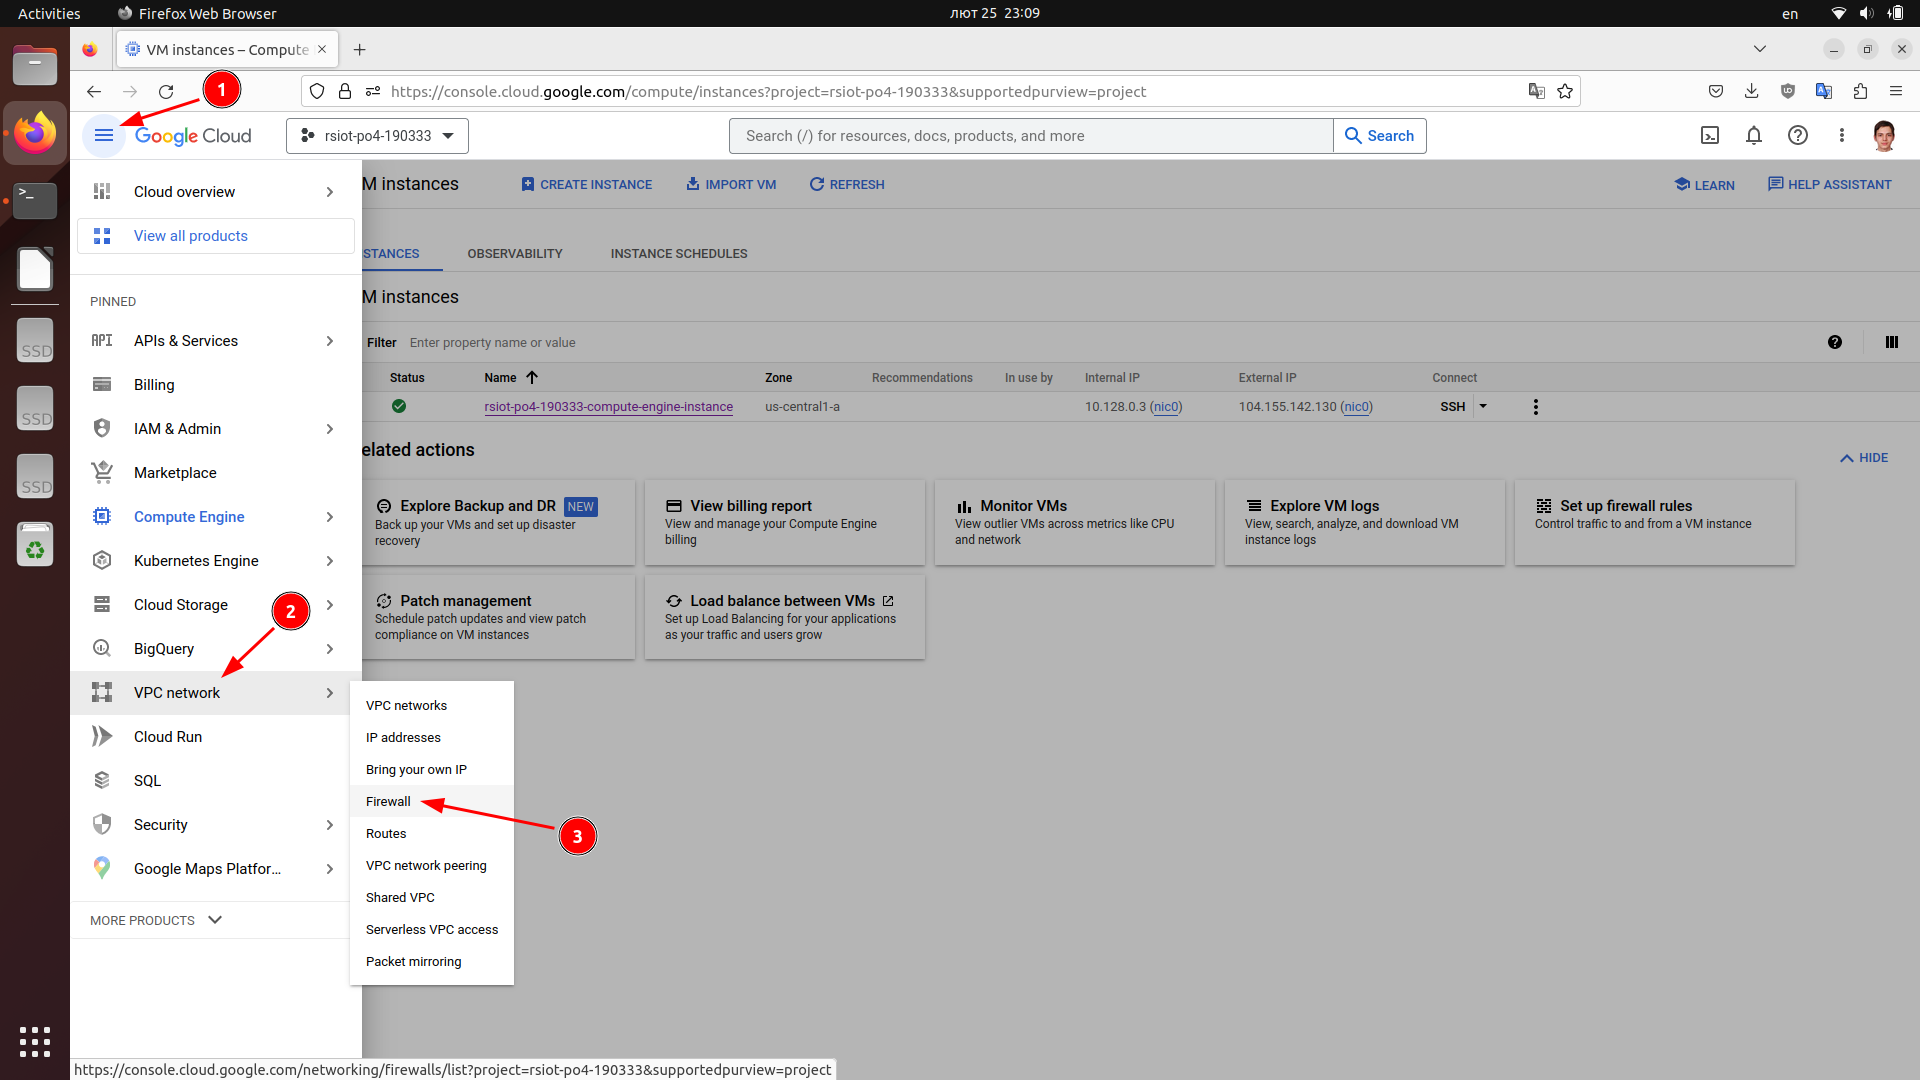
\includegraphics[width=11cm]
    {images/2023-02-25_23-09-26.png}
    \caption{\_}
    \label{fig:15}
  \end{figure}

  Жму <<CREATE FIREWALL RULE>> (см. рисунок~\ref{fig:16}).

  \begin{figure}[!h]
    \centering
    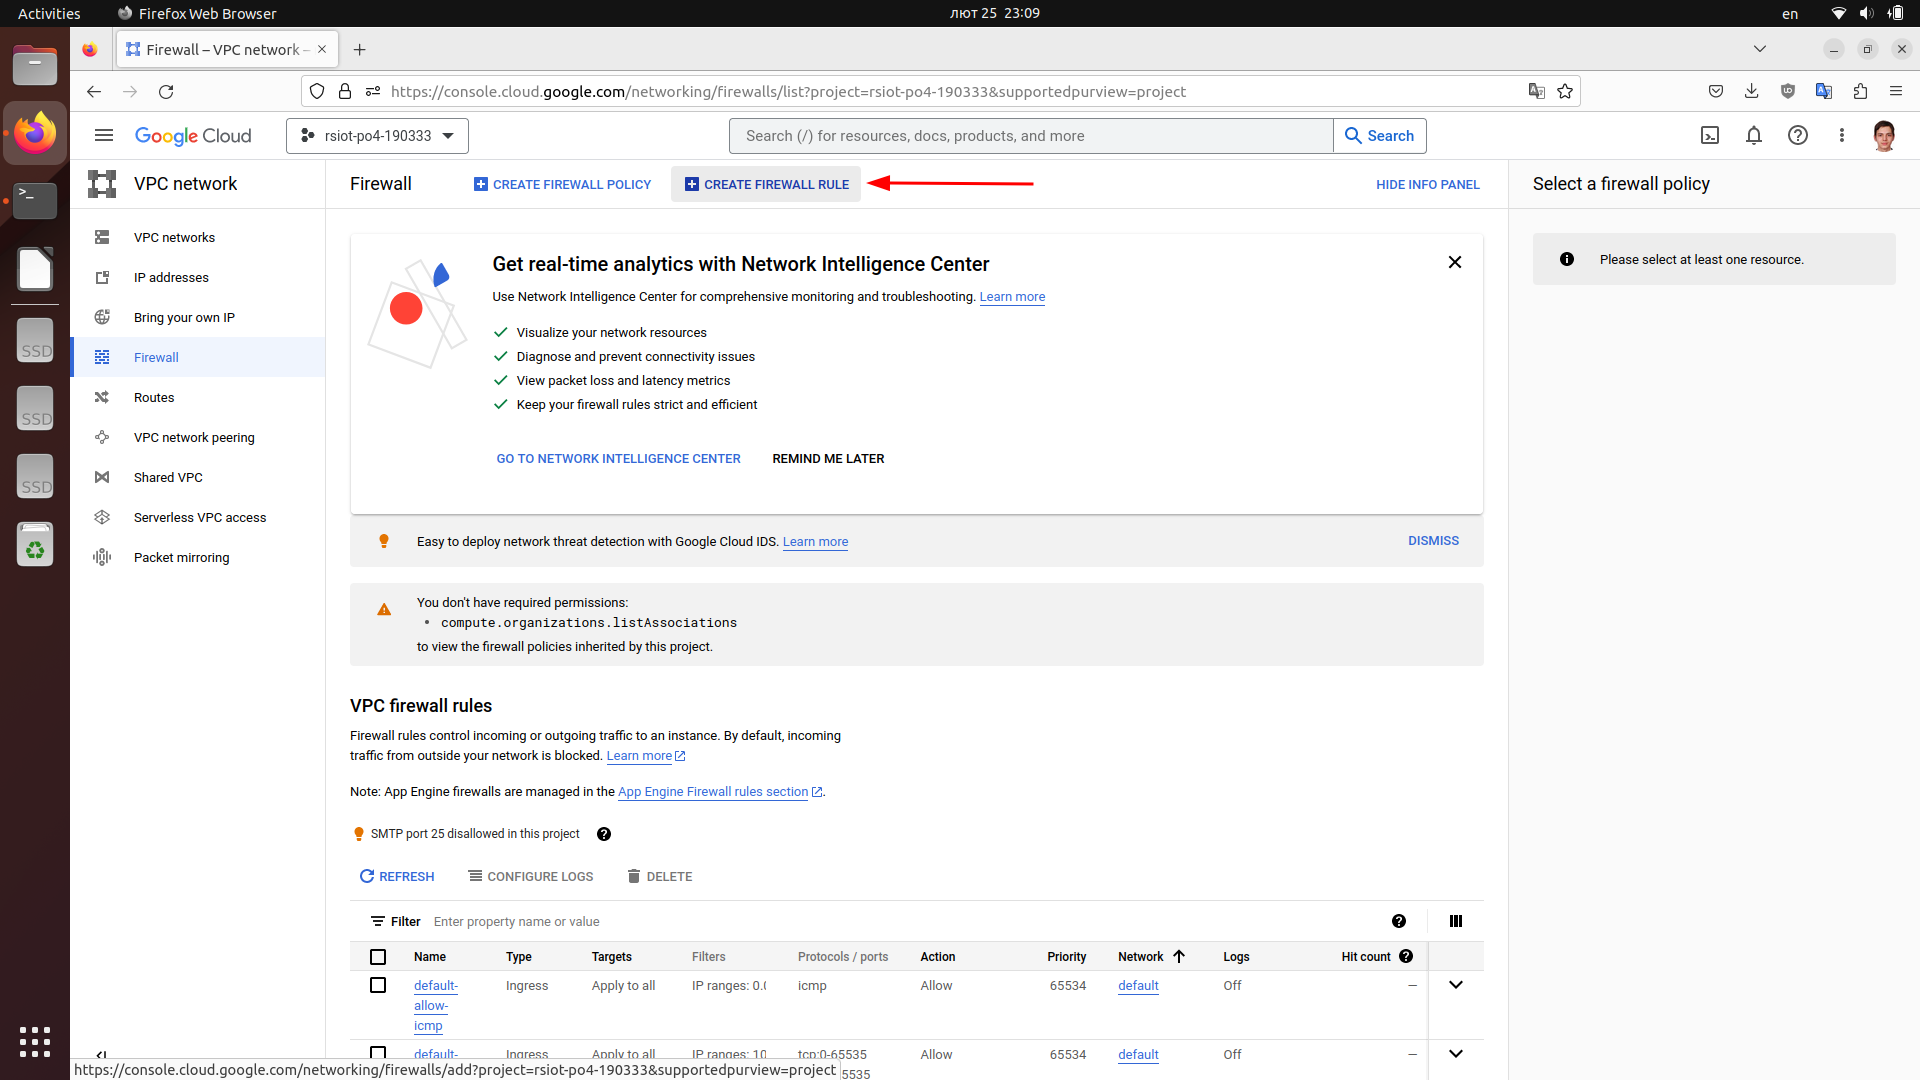
\includegraphics[width=11cm]
    {images/2023-02-25_23-09-57.png}
    \caption{\_}
    \label{fig:16}
  \end{figure}

  Name: \underline{rsiot-po4-190333-firewall-rule-for-nestjs}.

  Description: \underline{Nest JS}.

  Target: \underline{All instances in the network}.

  Source IPv4 ranges: \underline{0.0.0.0/0}.

  Protocols and ports: \underline{Specified protocols and ports}.

  TCP: \underline{80, 8080, 28080}.
  Перечисляем порты, по которым по ходит достучаться из другого компьютера.
  (см. рисунок~\ref{fig:17}).

  \begin{figure}[!h]
    \centering
    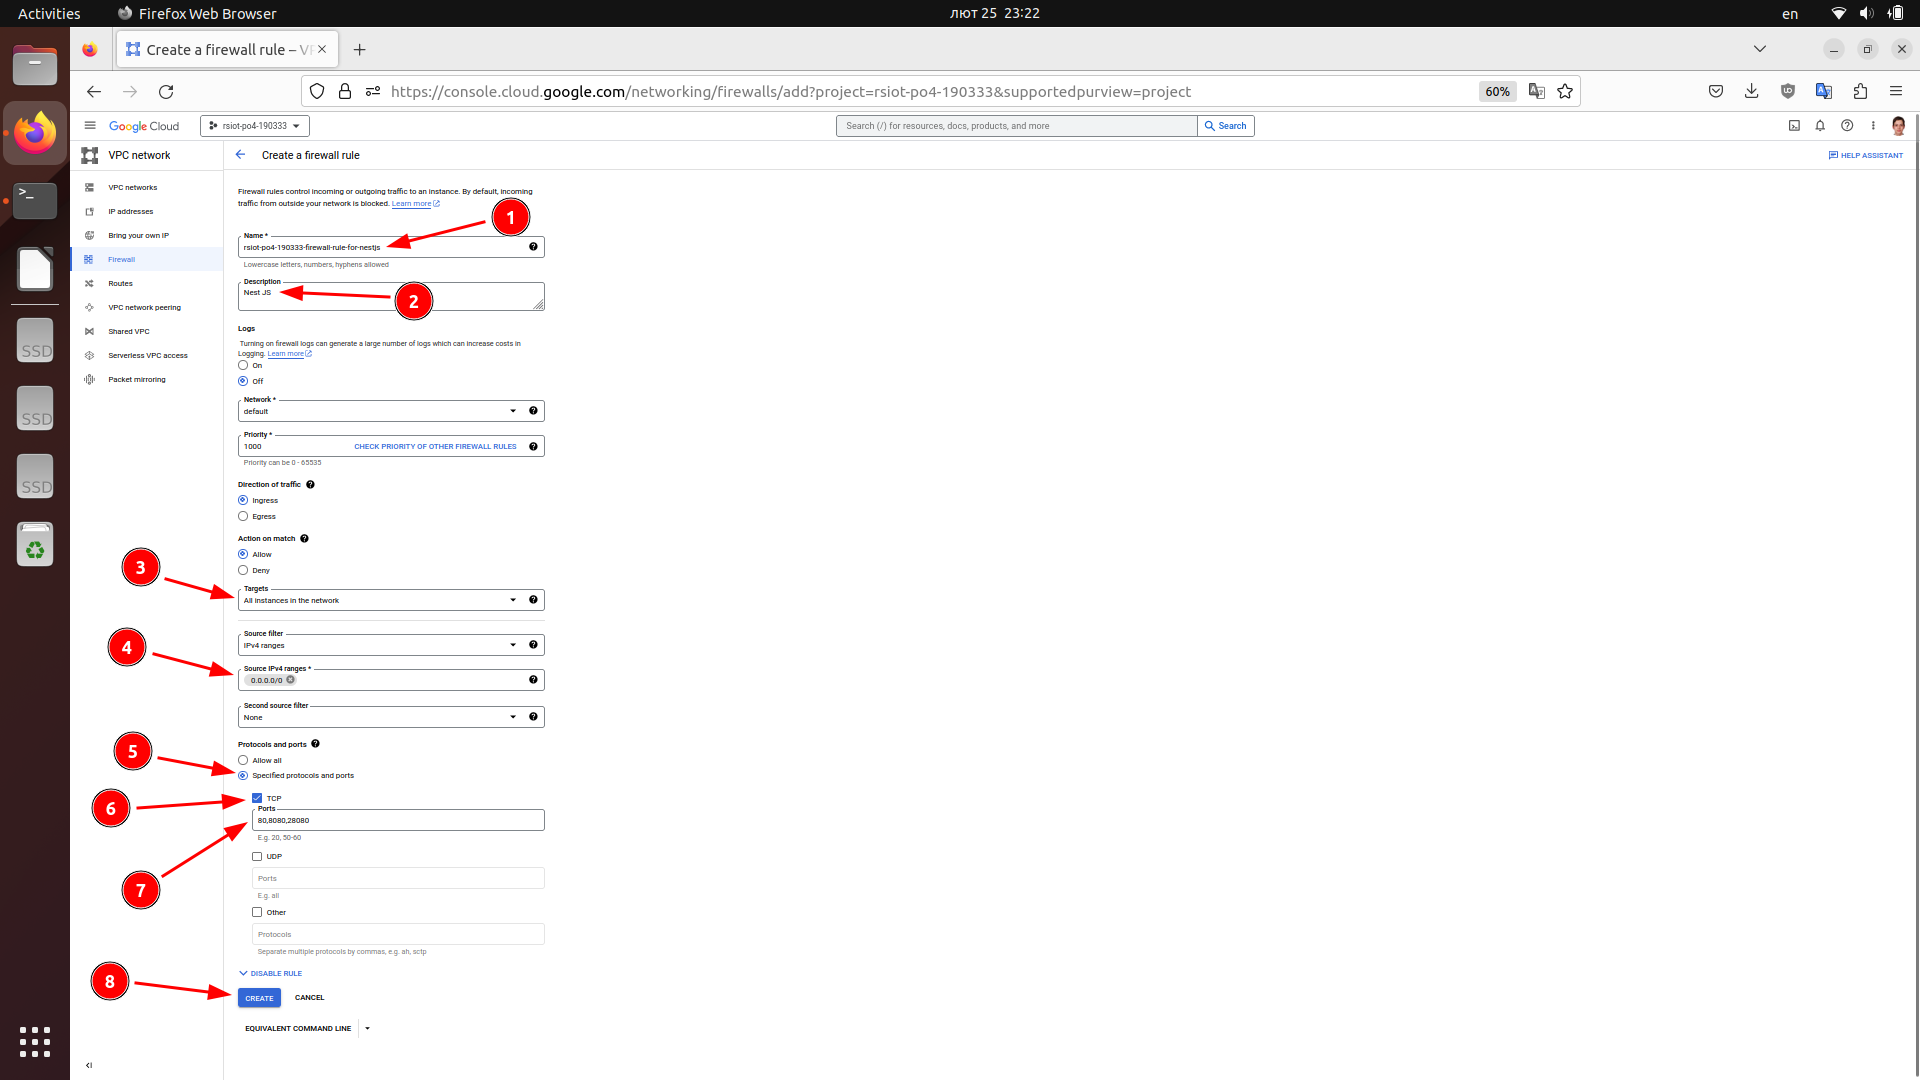
\includegraphics[width=18cm]
    {images/2023-02-25_23-23-21.png}
    \caption{\_}
    \label{fig:17}
  \end{figure}

  \newpage

  Проверить открытия портов можно используя nmap (см. рисунок~\ref{fig:18})

  \begin{lstlisting}[language=bash,name=Проверяю открыты ли порты через свой ноутбук пингуя IP из nmap]
    sudo apt update
    sudo apt install nmap
    
    nmap <external-ip-compute-engine> -p 1-65535
  \end{lstlisting}

  \begin{figure}[!h]
    \centering
    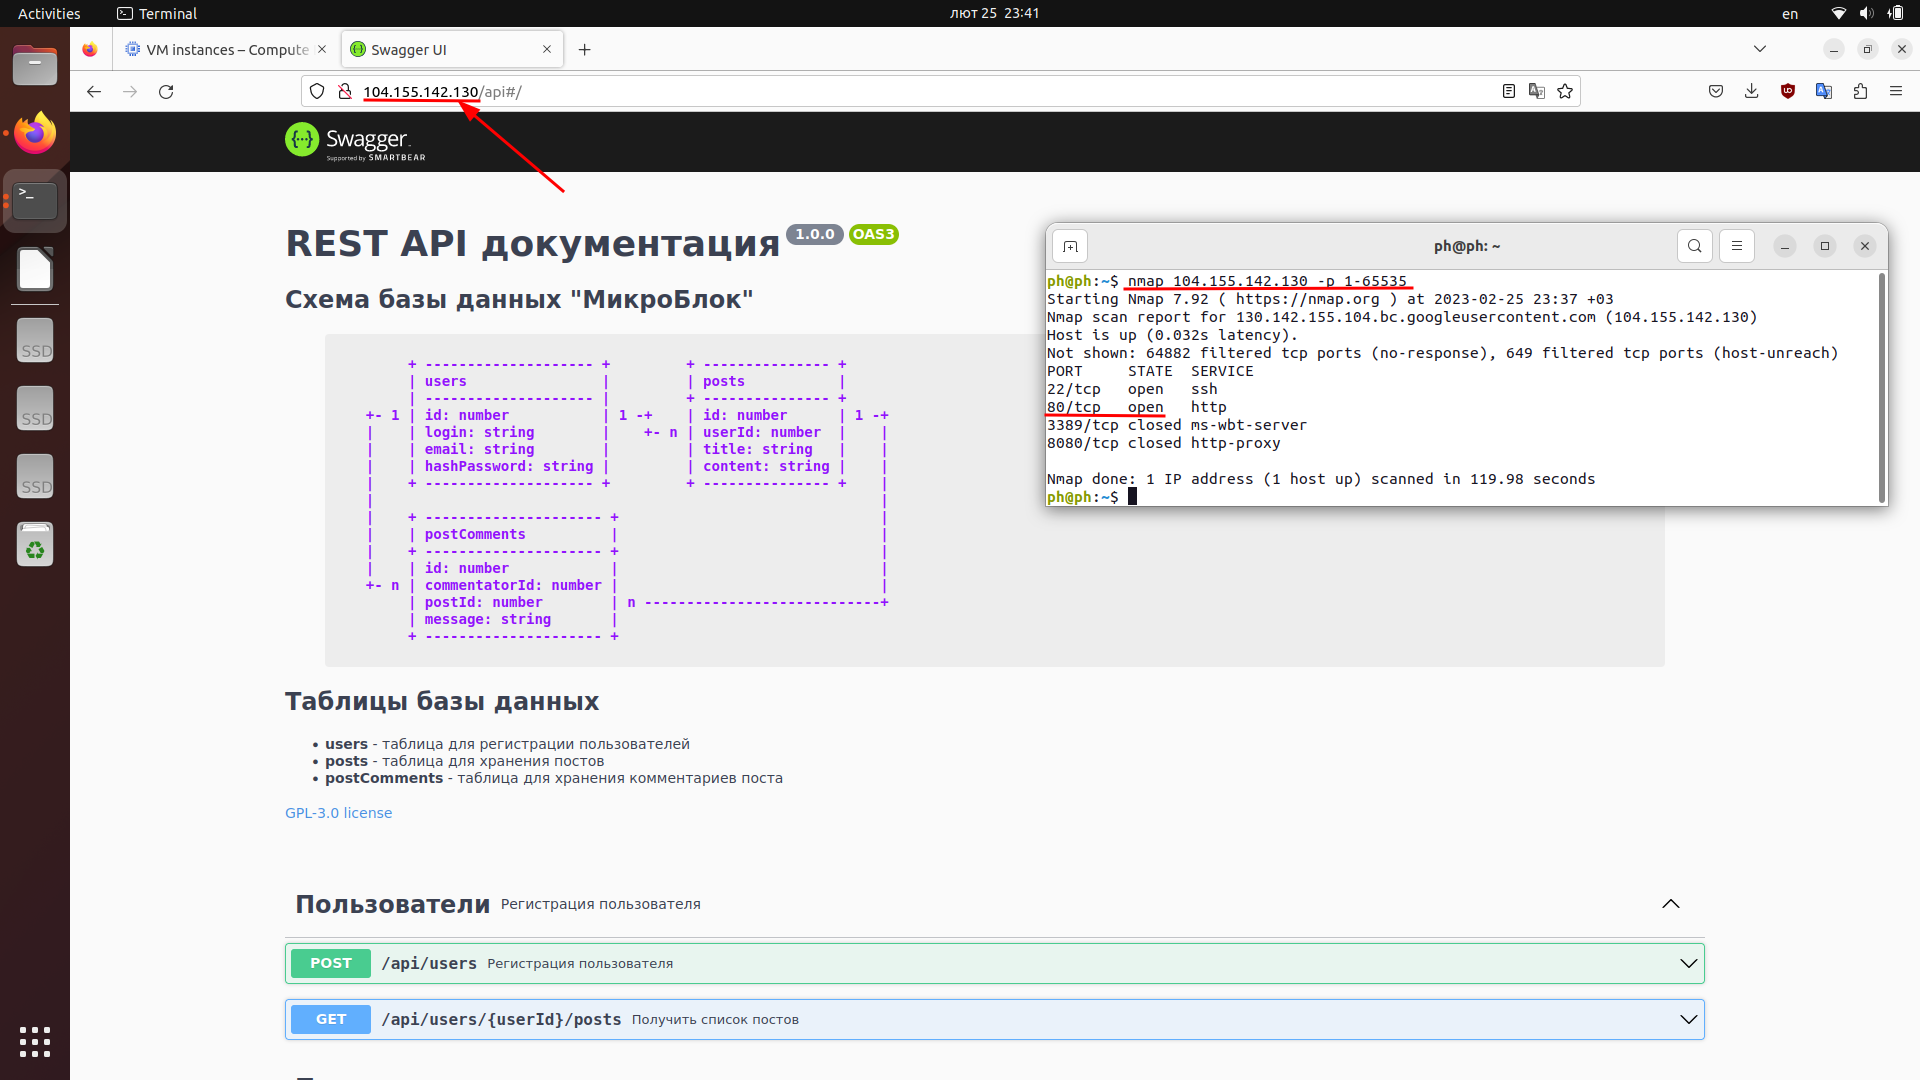
\includegraphics[width=16cm]
    {images/2023-02-25_23-42-18.png}
    \caption{\_}
    \label{fig:18}
  \end{figure}

  \newpage
  
  \textbf{Создание базы данных в Google Cloud SQL}

  Заходим на сайт Google Cloud Compute Engine \cite{GoogleCloudComputeEngine} (см. рисунок~\ref{fig:19}).

  \begin{figure}[!h]
    \centering
    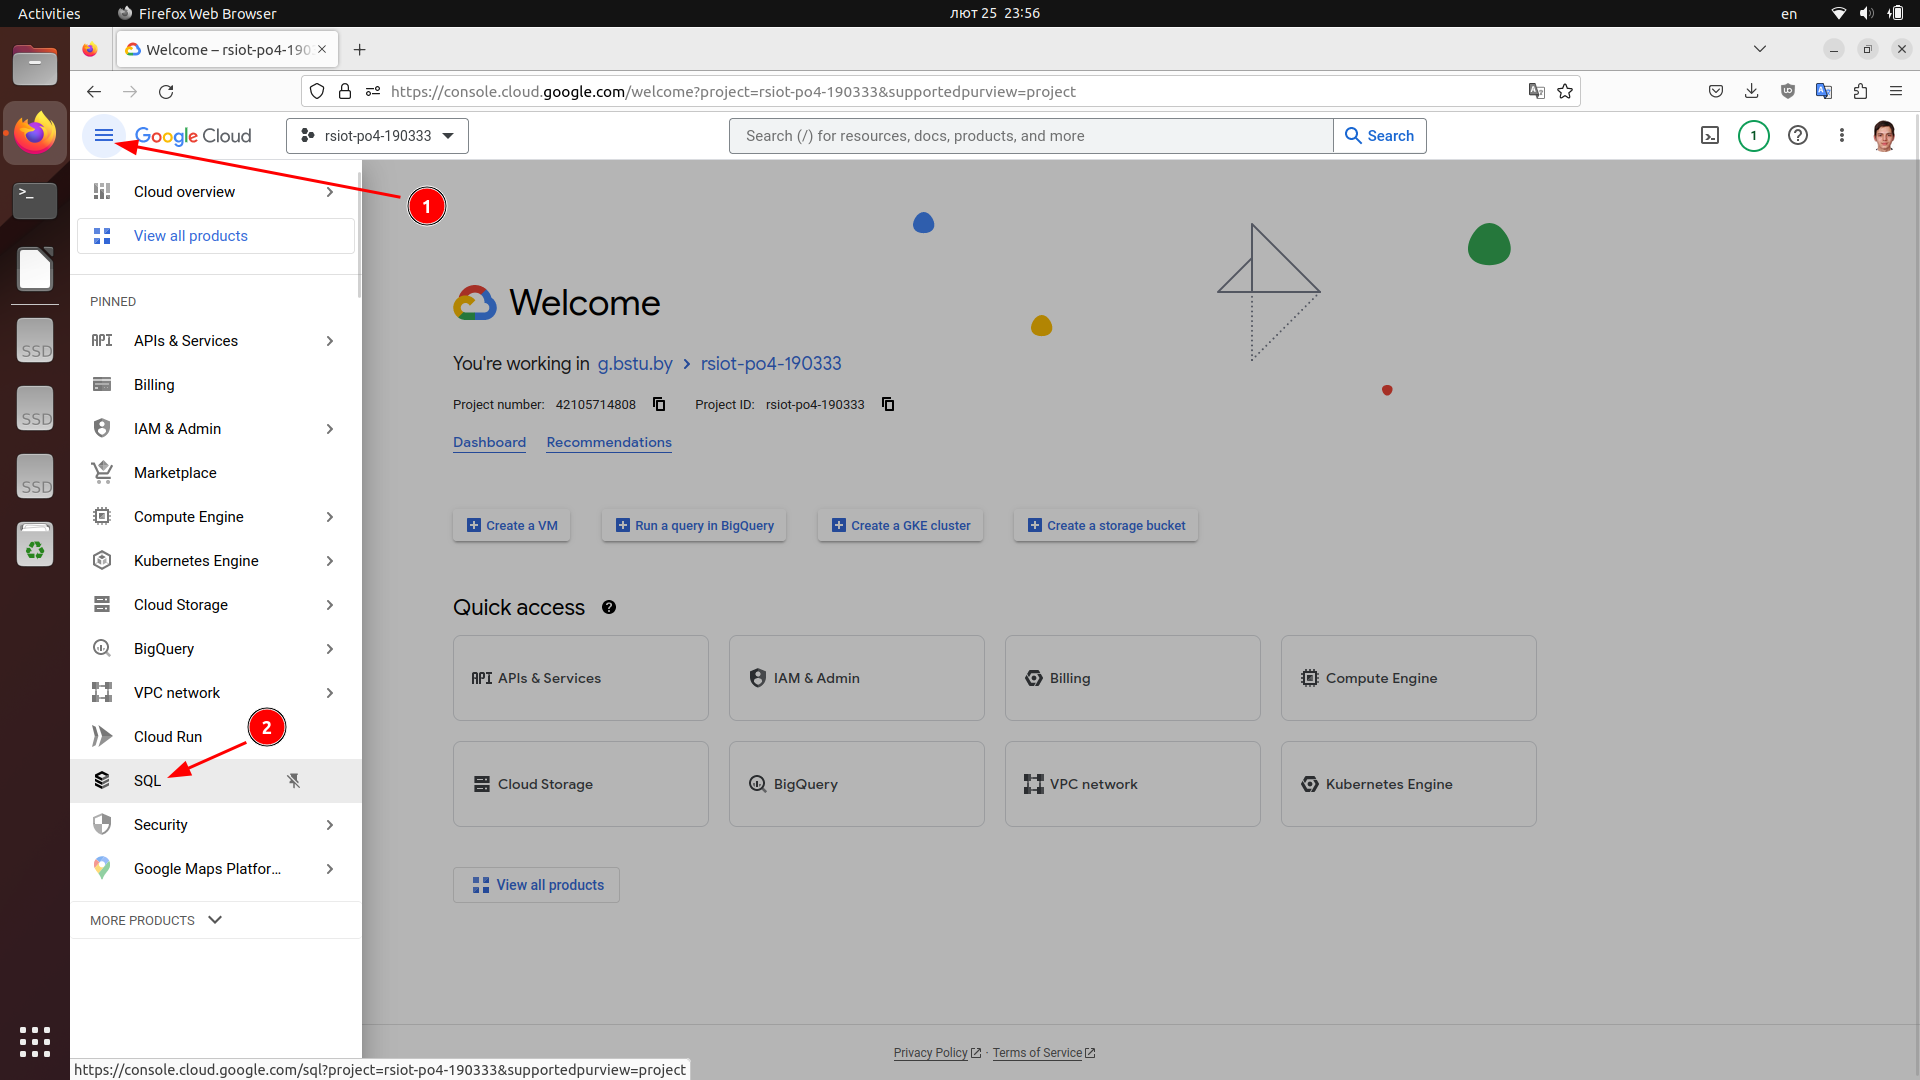
\includegraphics[width=11cm]
    {images/2023-02-25_23-57-13.png}
    \caption{\_}
    \label{fig:19}
  \end{figure}

  Жмём <<CREATE INSTANCE>> (см. рисунок~\ref{fig:20}).

  \begin{figure}[!h]
    \centering
    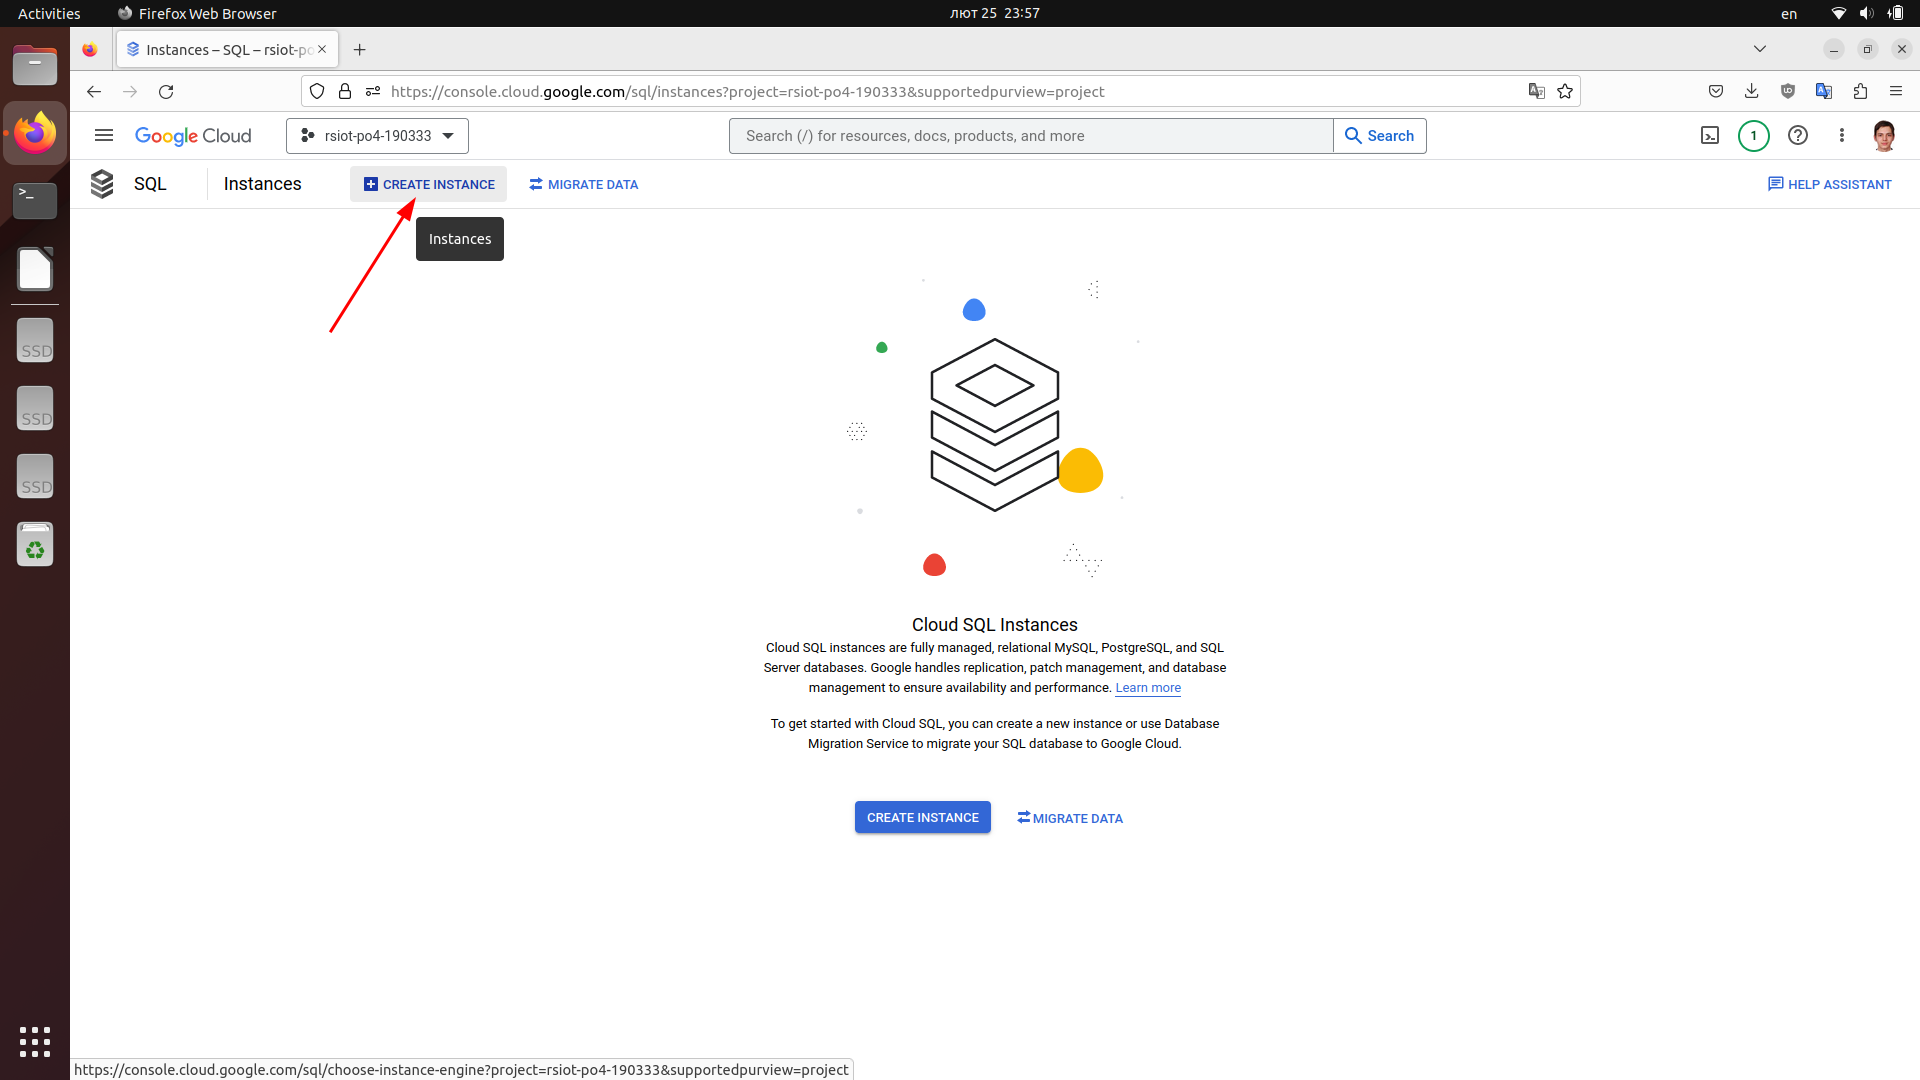
\includegraphics[width=11cm]
    {images/2023-02-25_23-57-47.png}
    \caption{\_}
    \label{fig:20}
  \end{figure}

  Жмём <<Choose PostgreSQL>> (см. рисунок~\ref{fig:21}).

  \begin{figure}[!h]
    \centering
    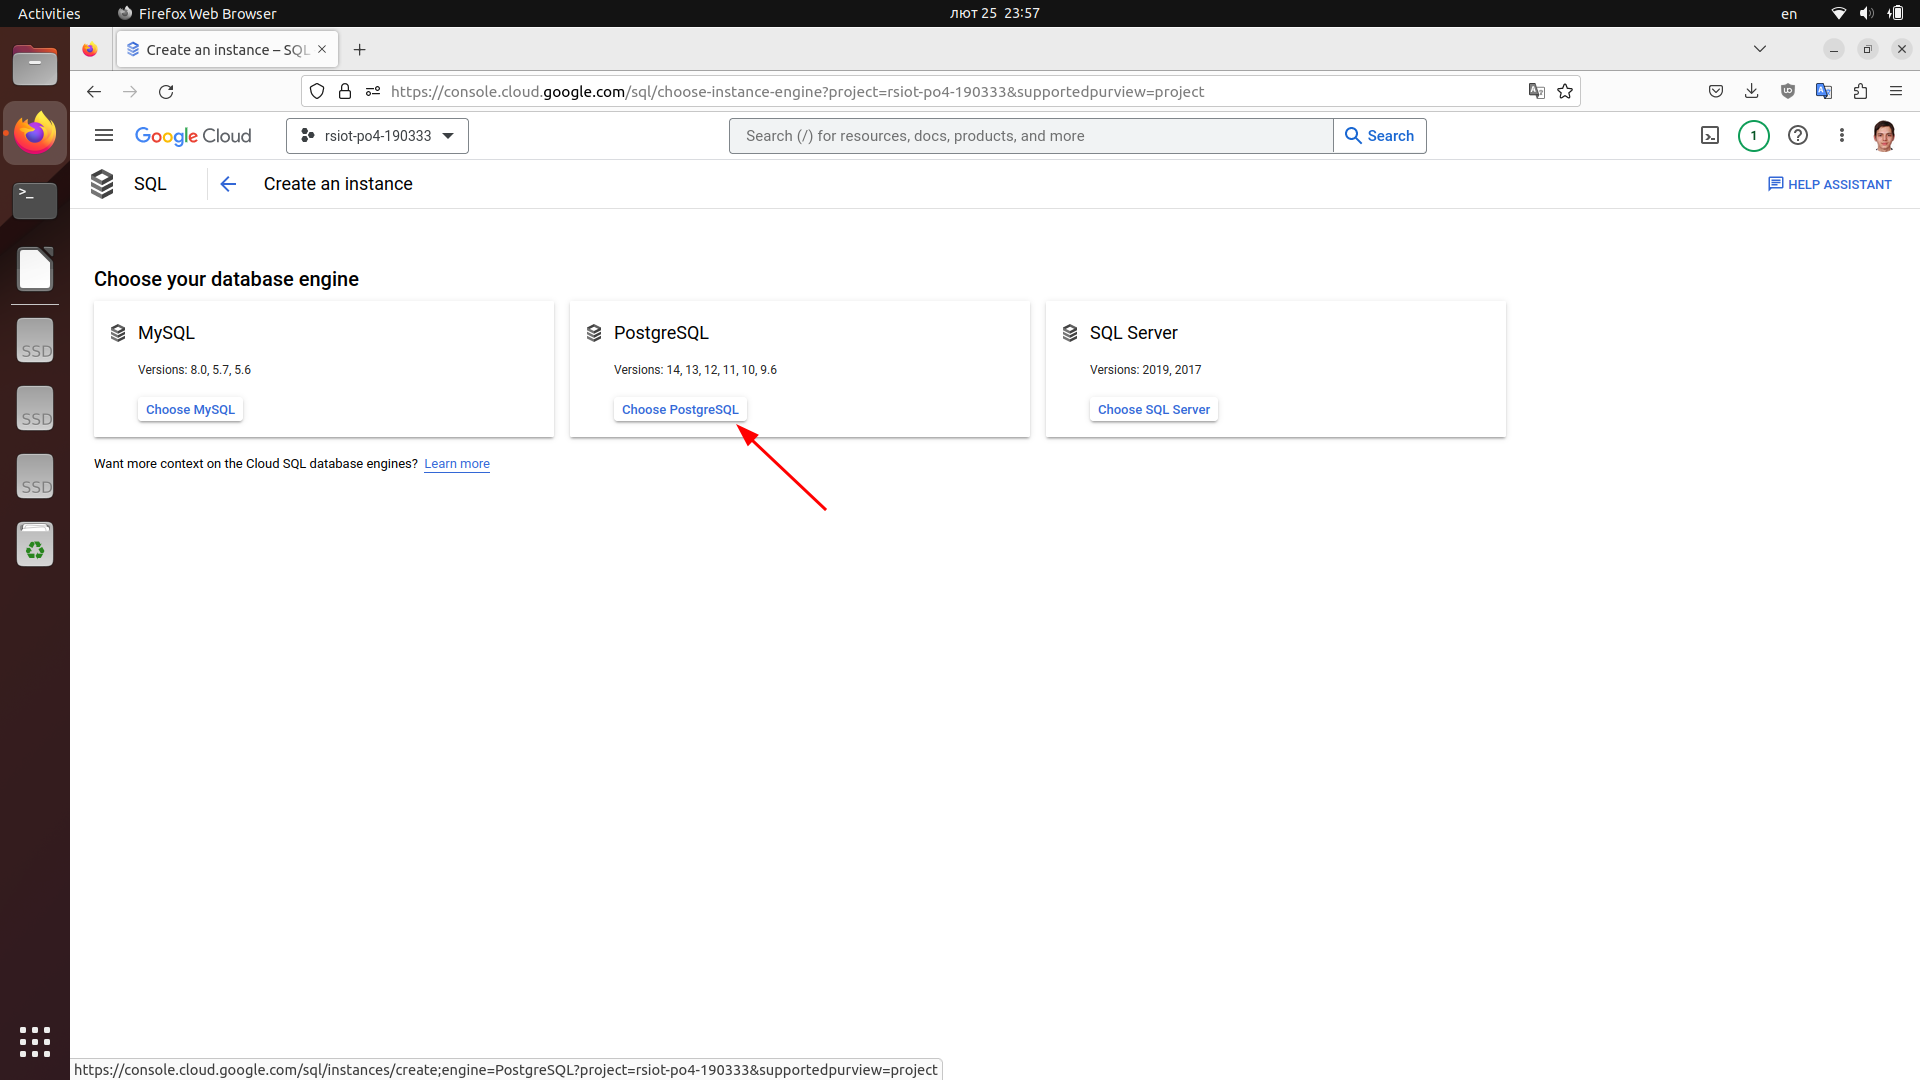
\includegraphics[width=11cm]
    {images/2023-02-25_23-58-04.png}
    \caption{\_}
    \label{fig:21}
  \end{figure}

  Instance ID: \underline{rsiot-po4-190333-postgresql-instance} (см. рисунок~\ref{fig:22}).

  Password: \underline{secret} (см. рисунок~\ref{fig:22}).

  CONFIGURATION DETAILS: \underline{Development} (чтобы меньше ситемные требования) (см. рисунок~\ref{fig:22}).

  \begin{figure}[!h]
    \centering
    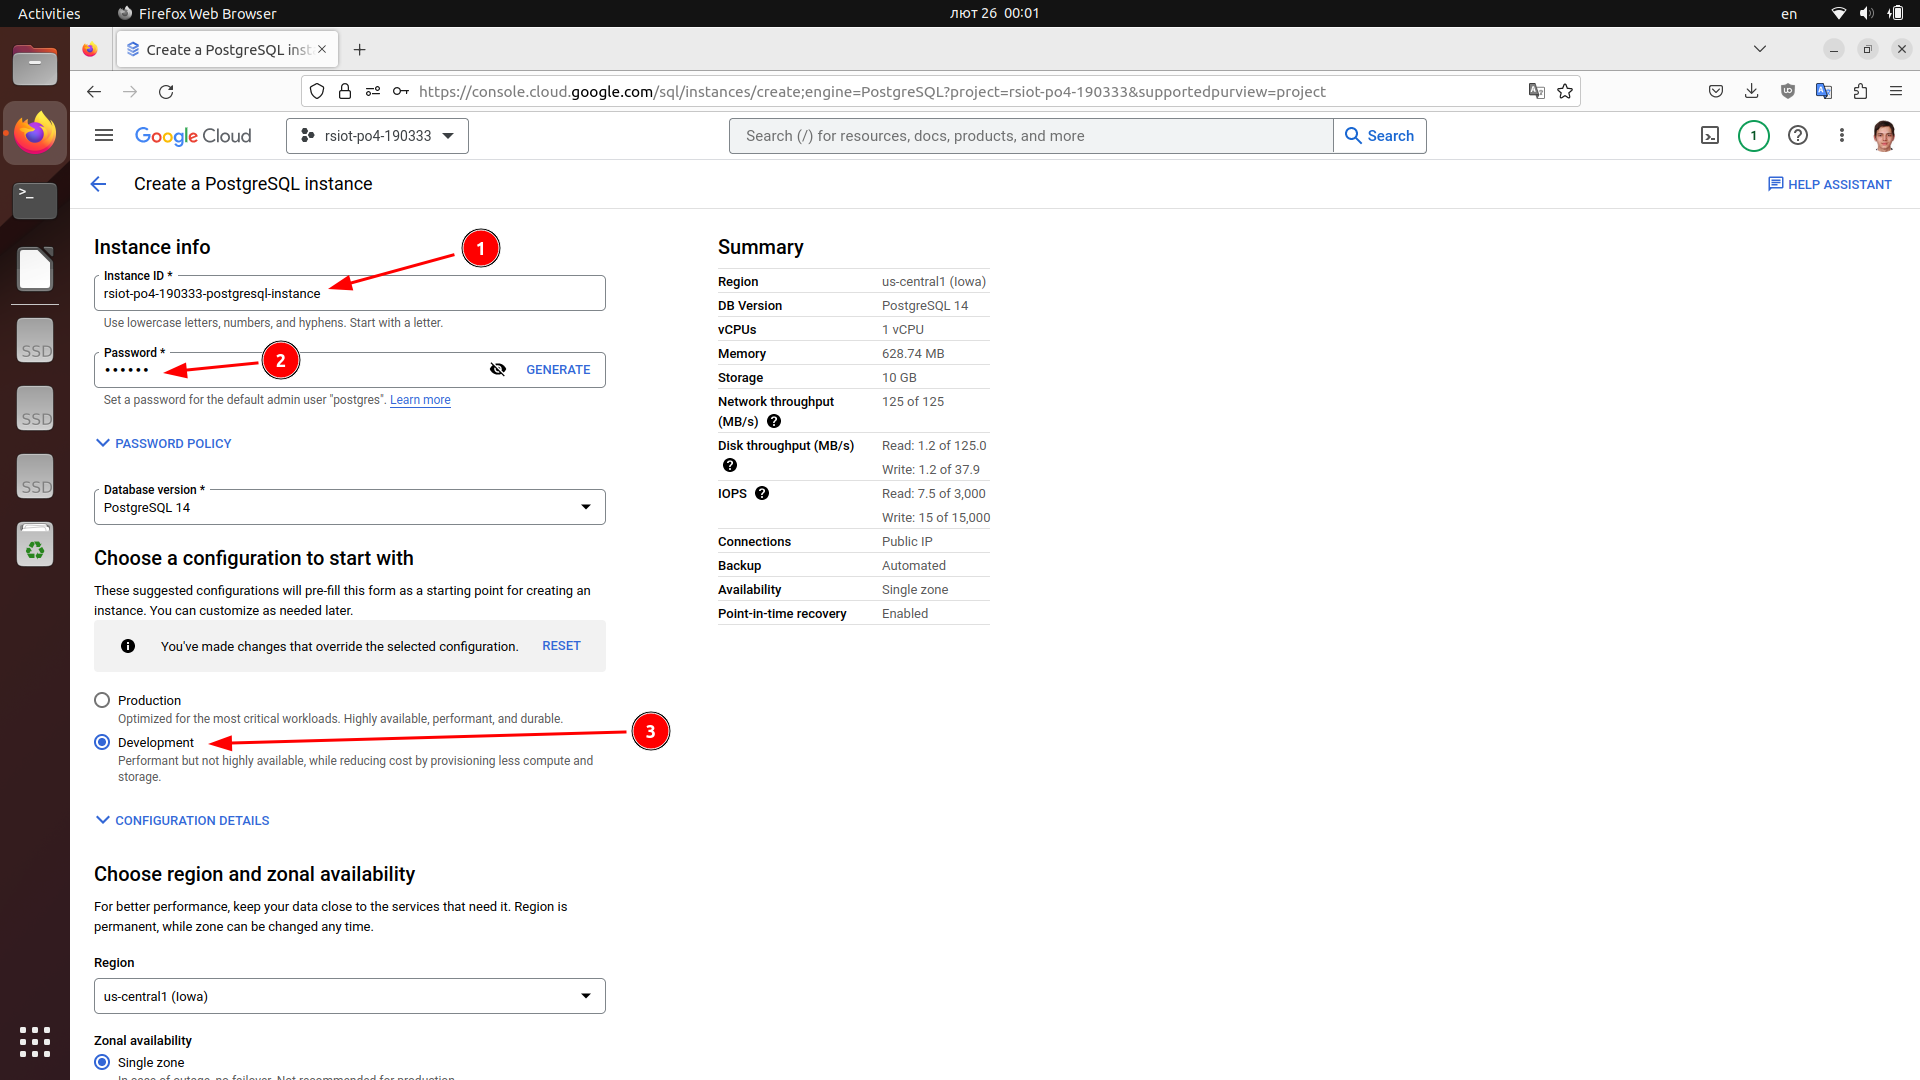
\includegraphics[width=16cm]
    {images/2023-02-26_00-01-36.png}
    \caption{\_}
    \label{fig:22}
  \end{figure}

  Machine Type: \underline{Shared Core}, \underline{1 vCPU, 0.614 GB} (см. рисунок~\ref{fig:23}).

  Storage Type: \underline{HDD} (см. рисунок~\ref{fig:23}).

  Storage capacity: \underline{10 GB} (см. рисунок~\ref{fig:23}).

  Enable automatic storage increases: \underline{false} (см. рисунок~\ref{fig:23}).

  \begin{figure}[!h]
    \centering
    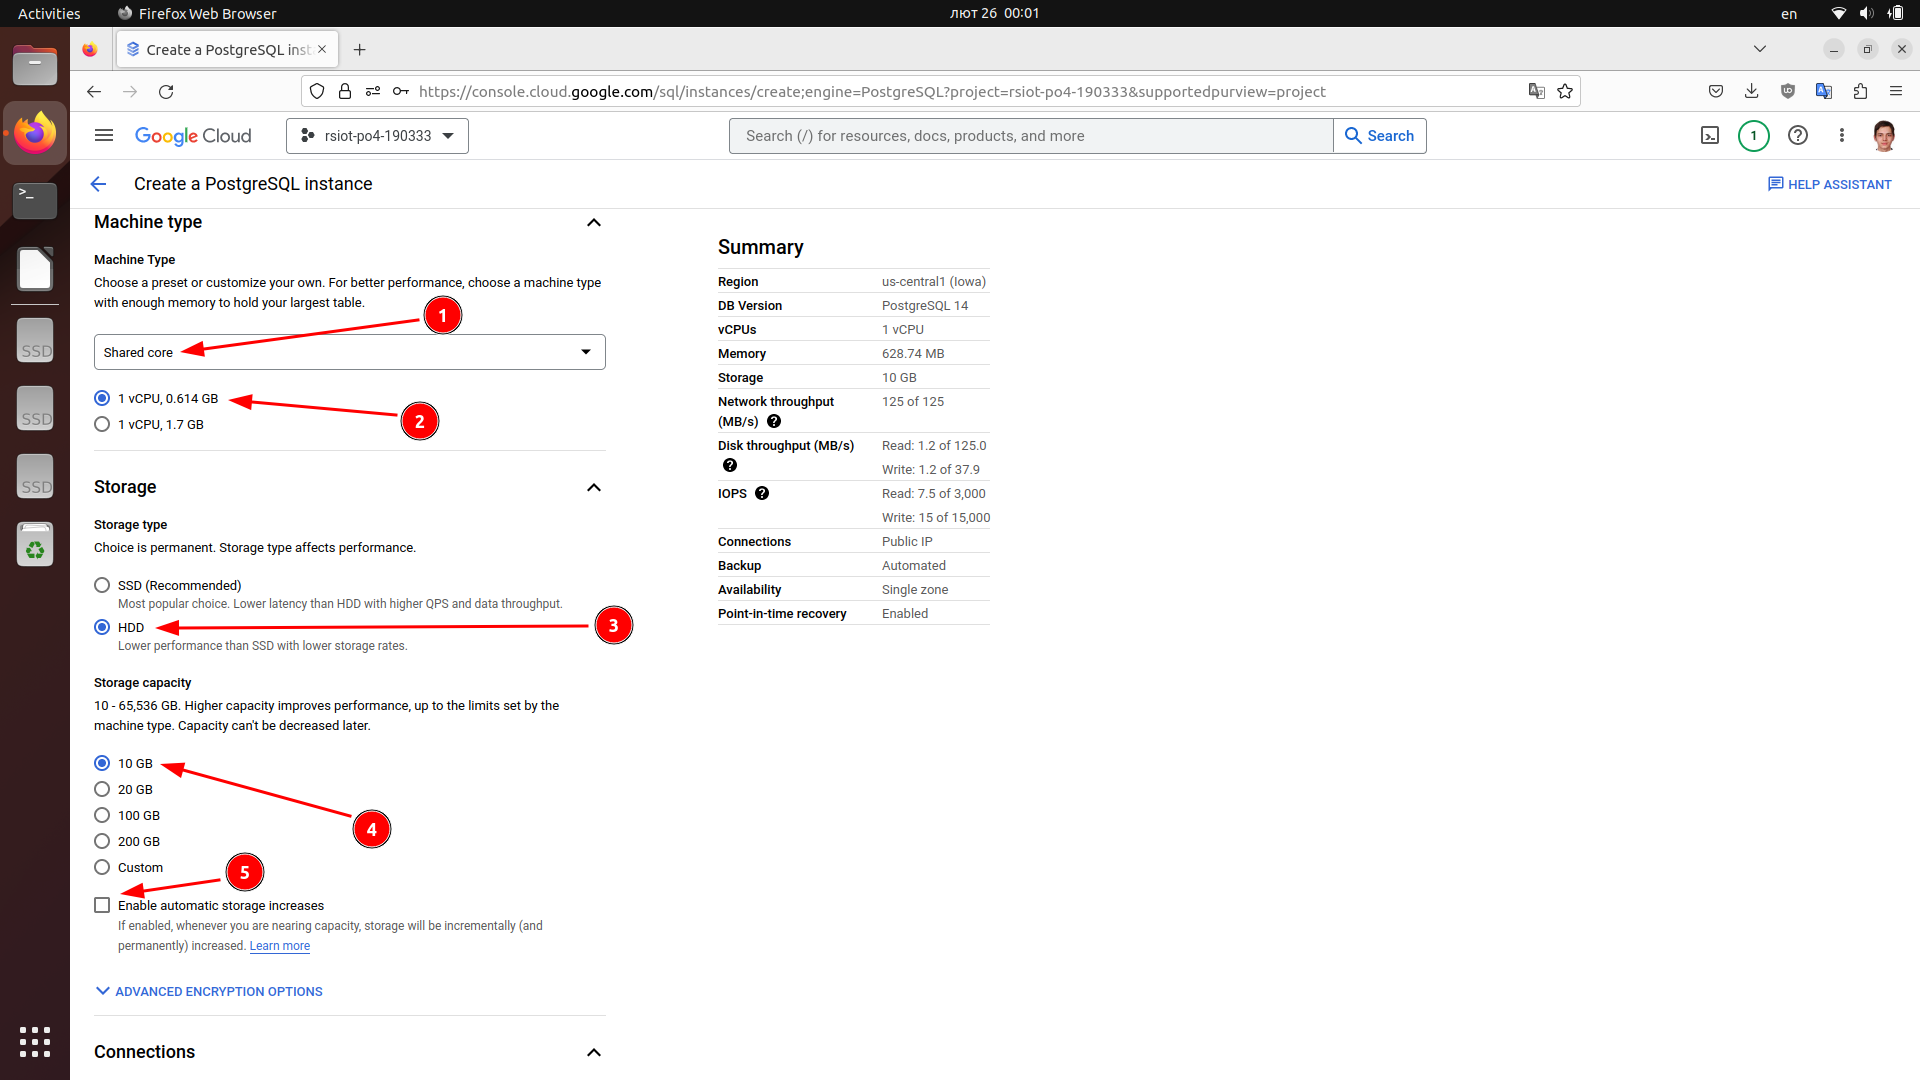
\includegraphics[width=16cm]
    {images/2023-02-26_00-02-31.png}
    \caption{\_}
    \label{fig:23}
  \end{figure}

  Authorized networks (см. рисунок~\ref{fig:24}).

  Name: \underline{Compute Engine NestJS} (см. рисунок~\ref{fig:24}).

  Network: \underline{<external-ip-compute-engine>} (см. рисунок~\ref{fig:24}).

  \begin{figure}[!h]
    \centering
    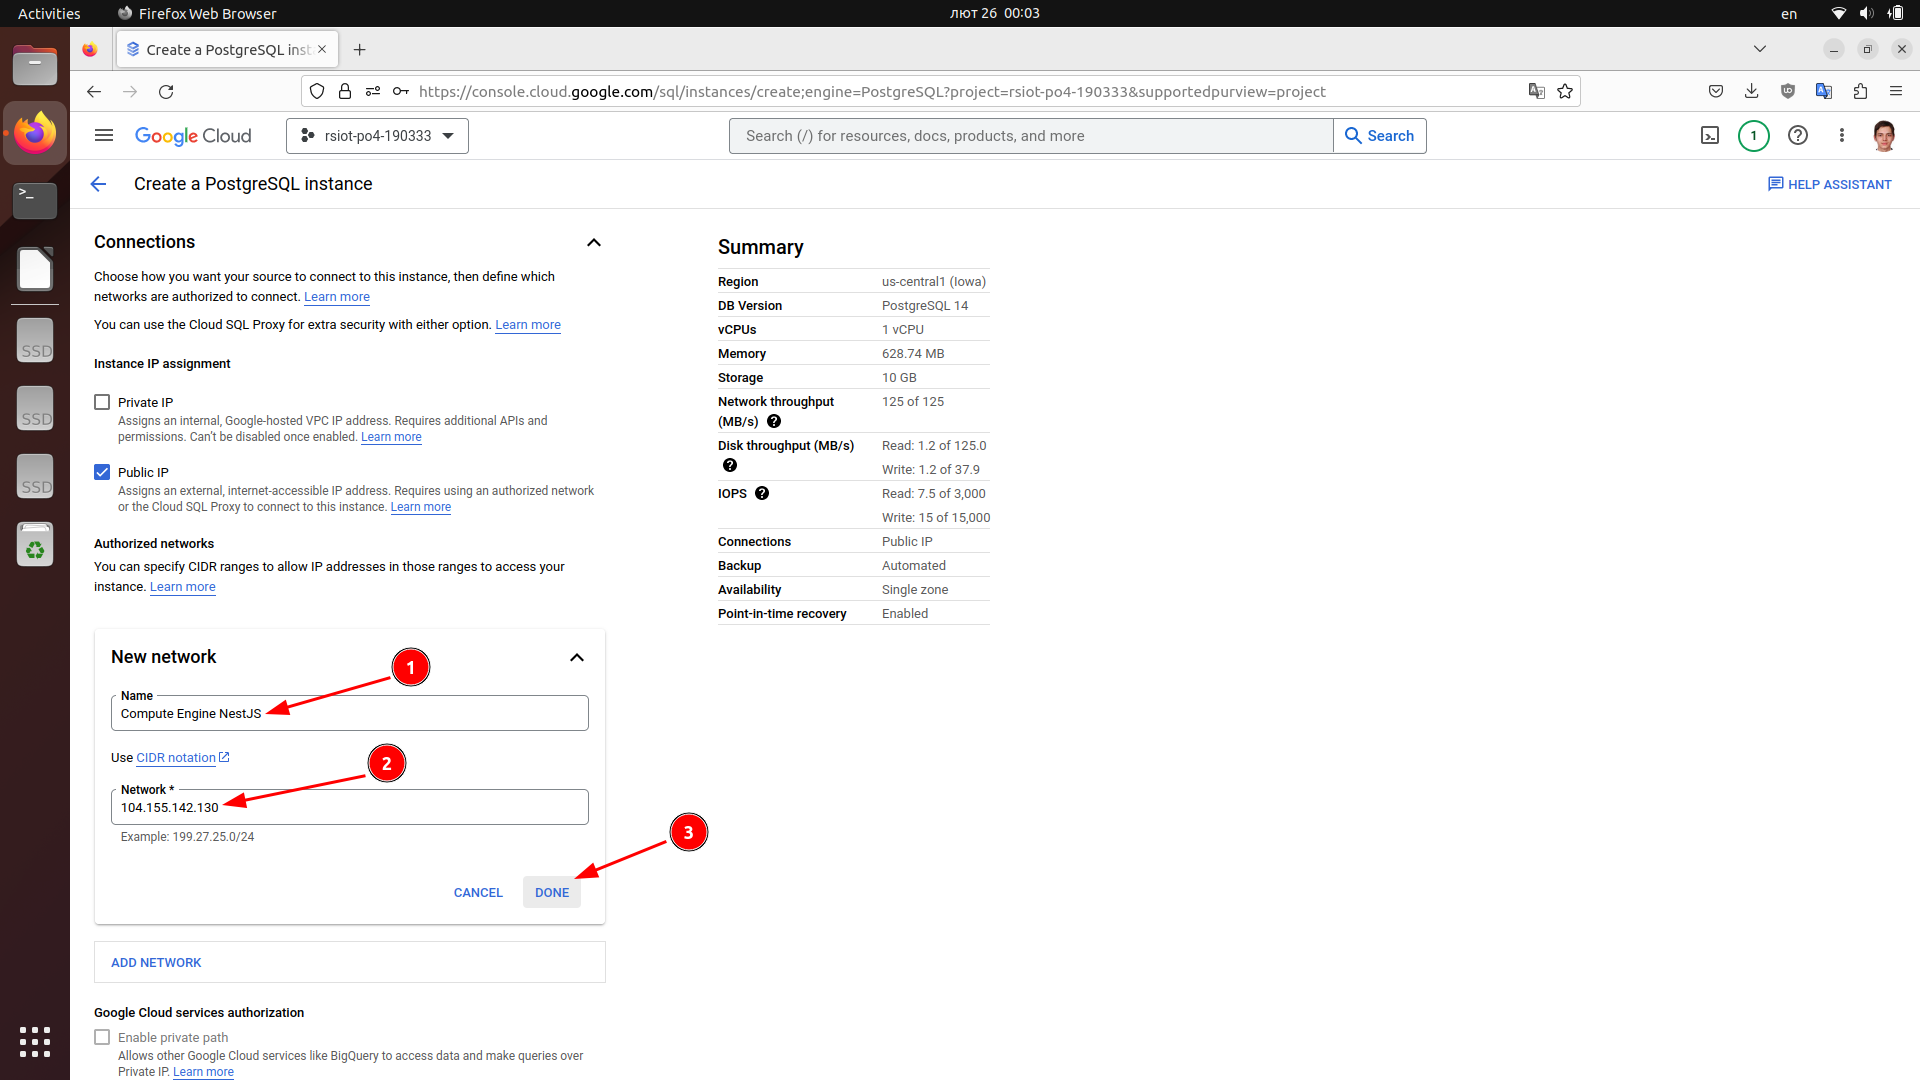
\includegraphics[width=11cm]
    {images/2023-02-26_00-03-30.png}
    \caption{\_}
    \label{fig:24}
  \end{figure}

  Жму <<CREATE INSTANCE>> (см. рисунок~\ref{fig:25}).

  \begin{figure}[!h]
    \centering
    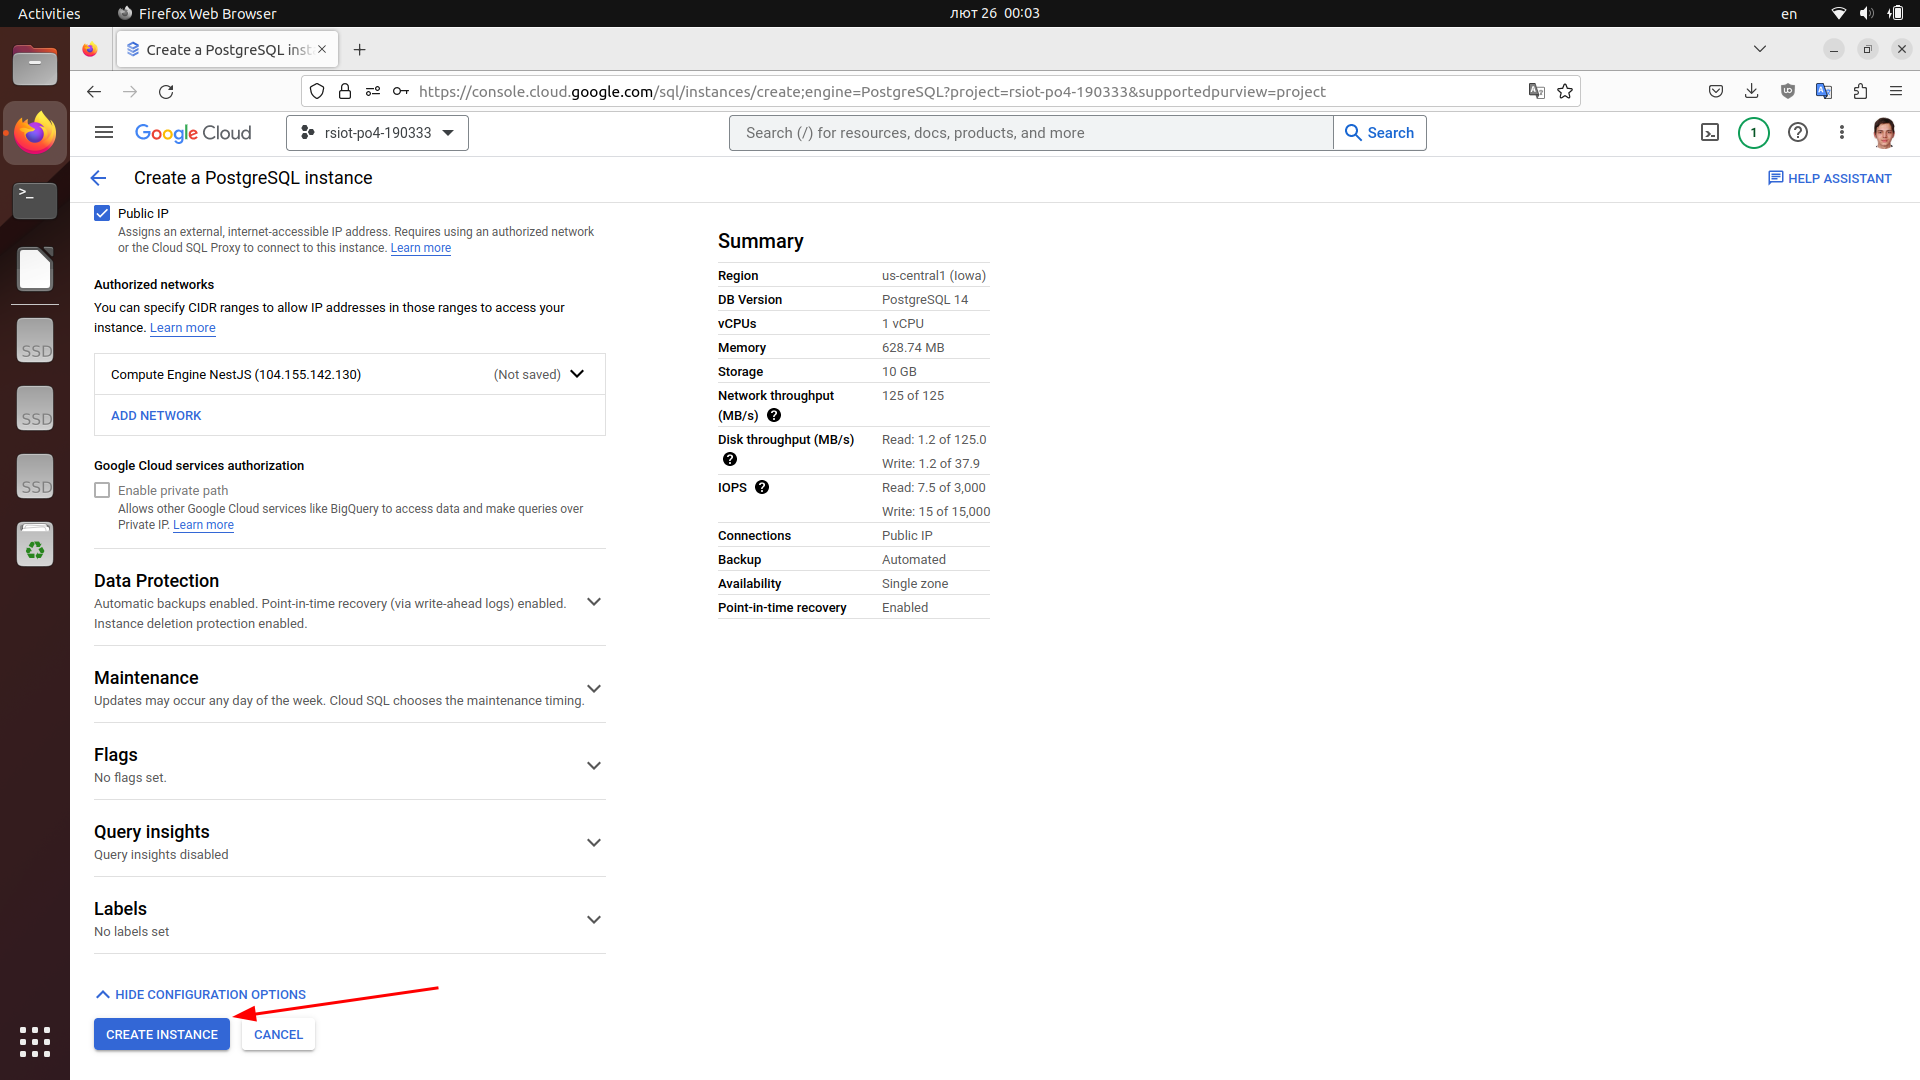
\includegraphics[width=11cm]
    {images/2023-02-26_00-03-55.png}
    \caption{\_}
    \label{fig:25}
  \end{figure}

  База данных создавалась больше 30 минут (см. рисунок~\ref{fig:26}). Жмём до тех пор, пока не появится зелённая галочка (см. рисунок~\ref{fig:27}).

  \begin{figure}[!h]
    \centering
  
    \begin{minipage}{0.49\textwidth}
      \centering
  
      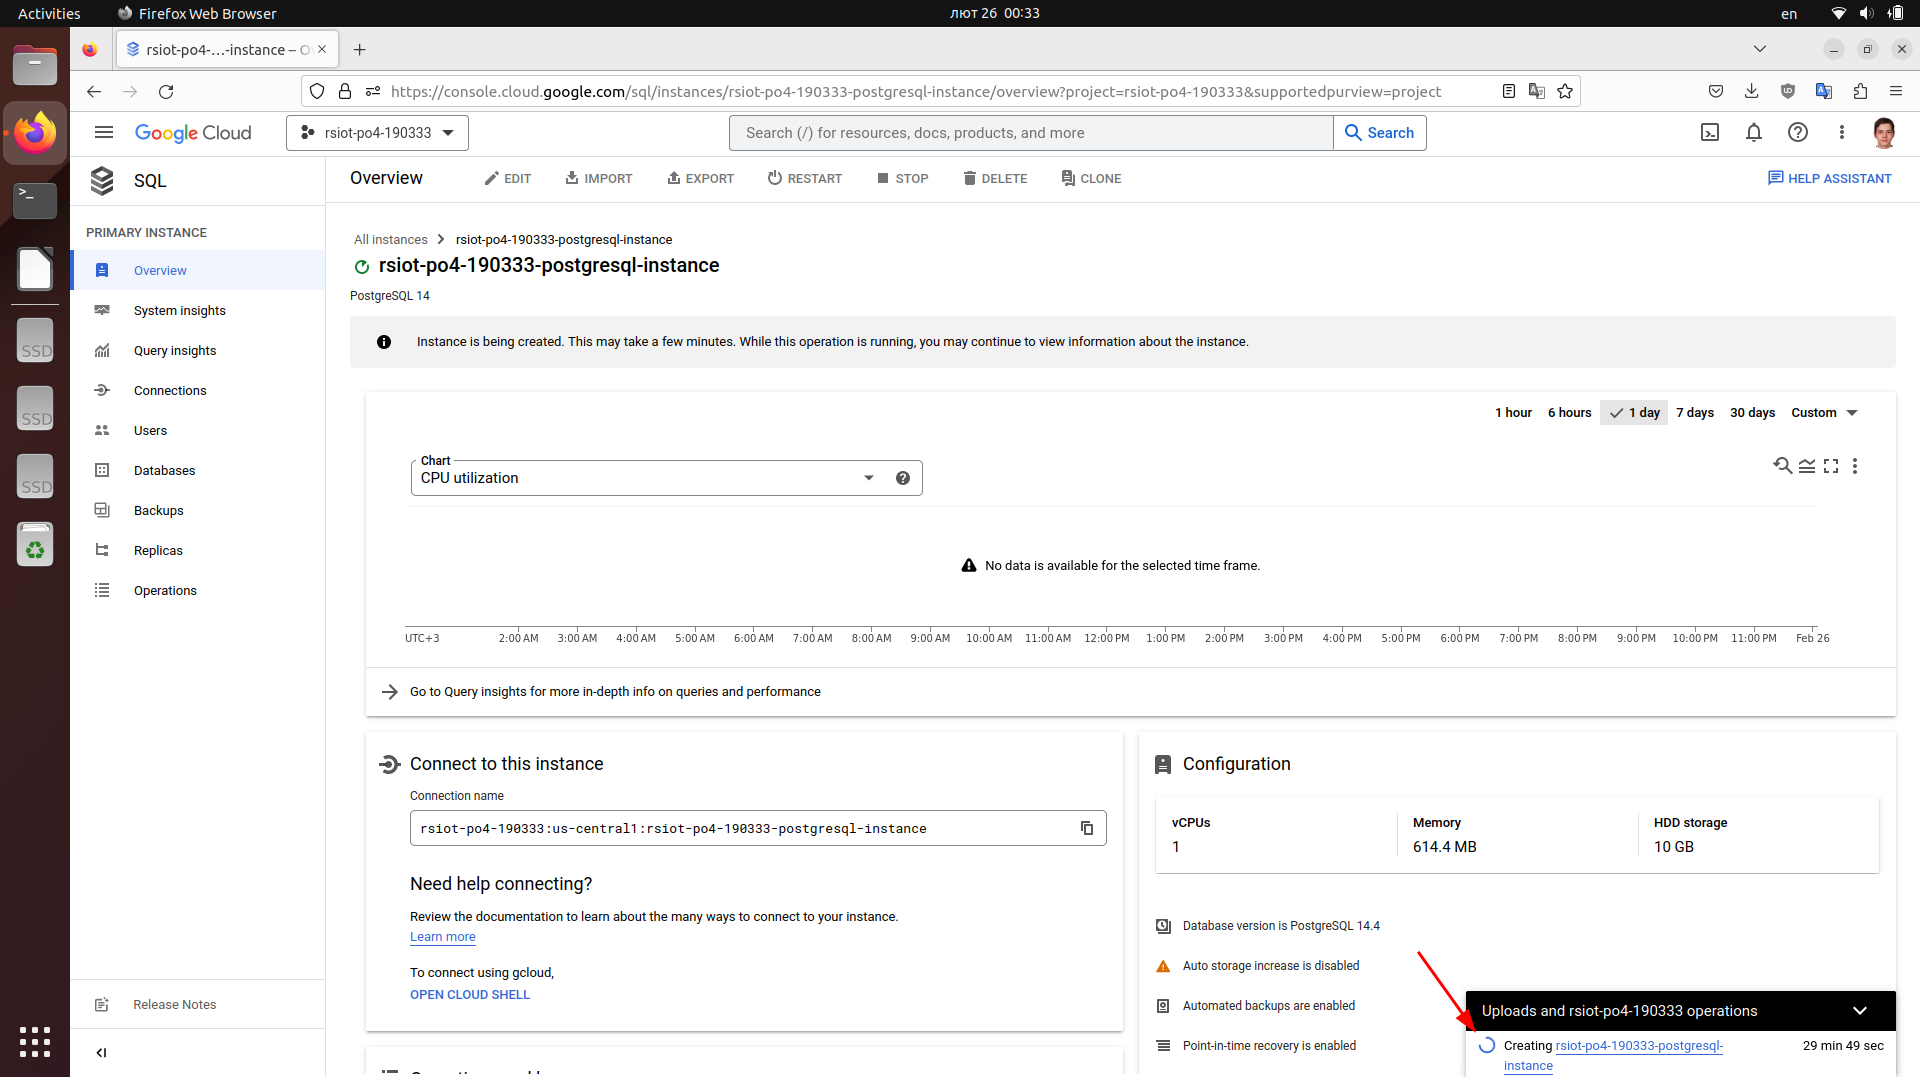
\includegraphics[height=5cm]
      {images/2023-02-26_00-34-01.png}
  
      \caption{\_}
  
      \label{fig:26}
    \end{minipage}
    \begin{minipage}{0.49\textwidth}
      \centering
  
      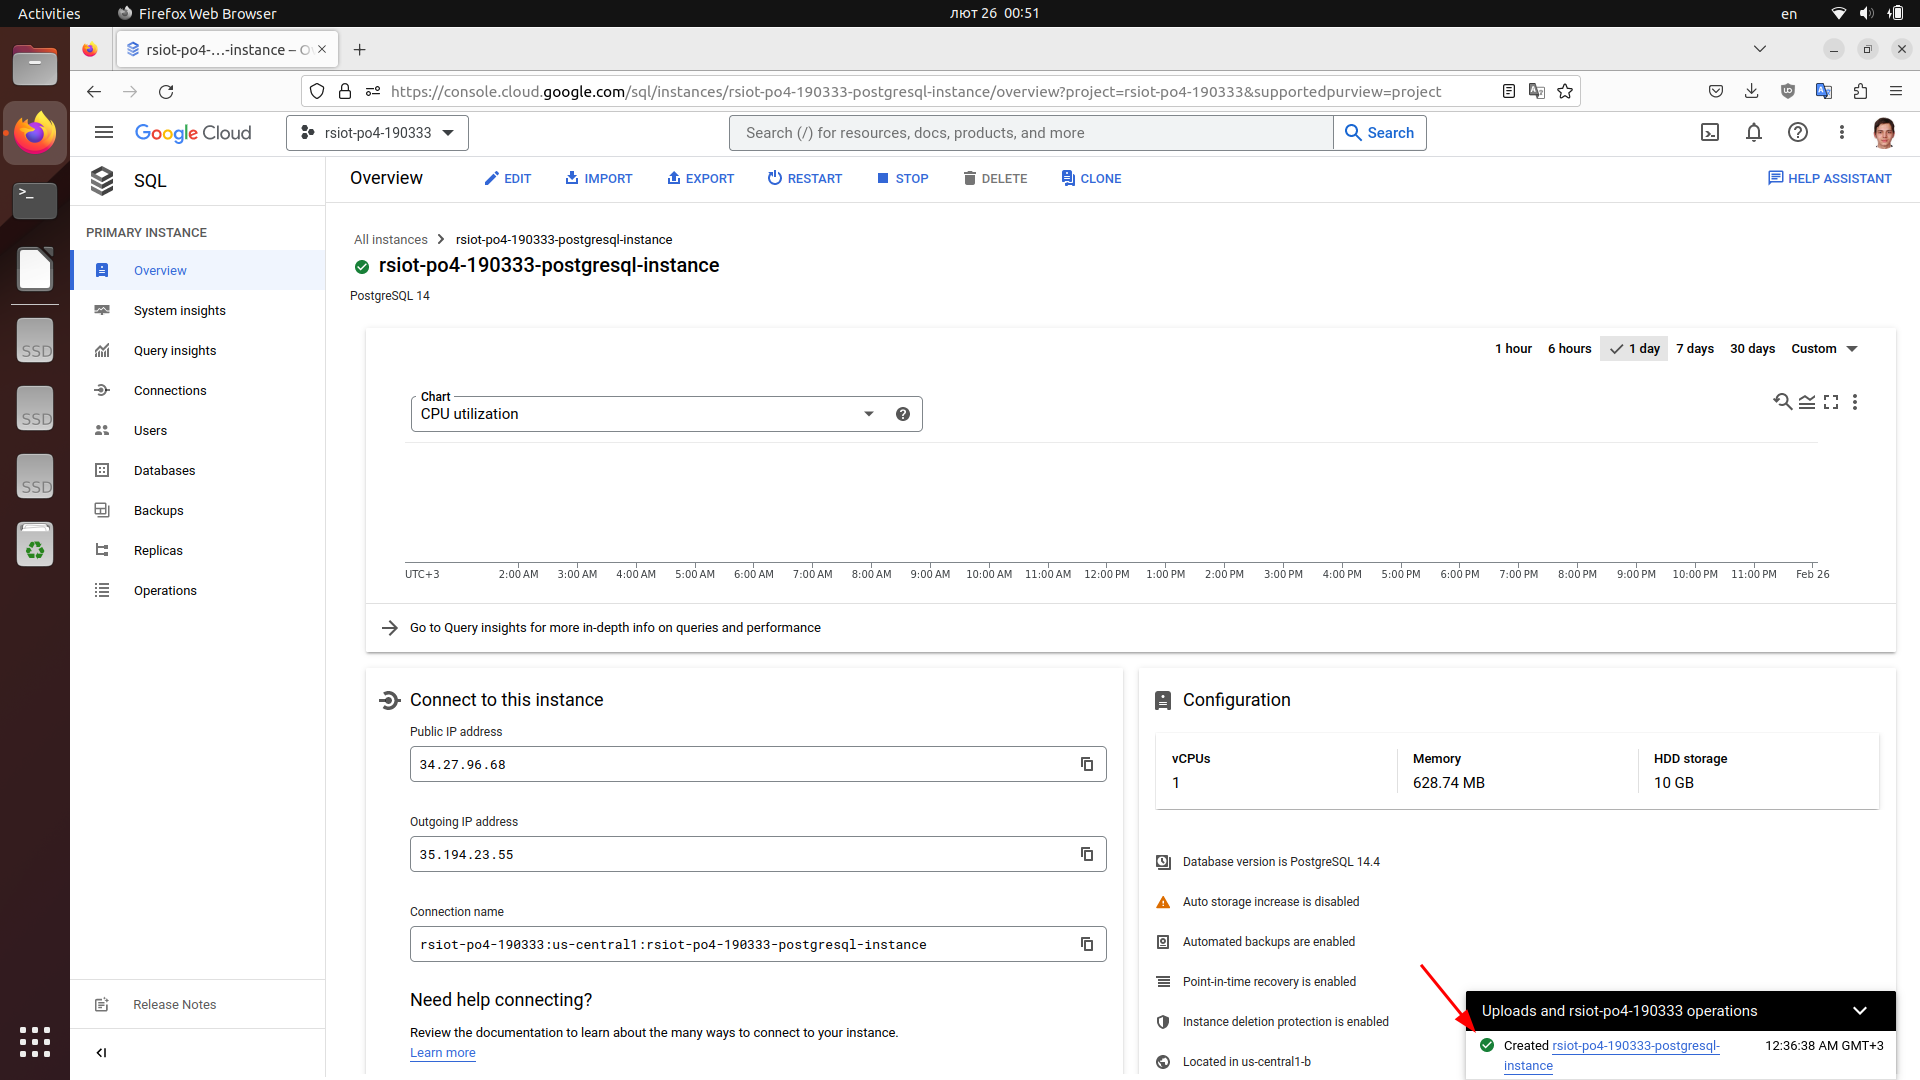
\includegraphics[height=5cm]
      {images/2023-02-26_00-51-17.png}
  
      \caption{\_}
  
      \label{fig:27}
    \end{minipage}
  \end{figure}

  Заходим на сайт Google Cloud SQL \cite{GoogleCloudSql} (см. рисунок~\ref{fig:28}).

  Жмём по имени: \underline{rsiot-po4-190333-postgresql-instance}.
  \begin{figure}[!h]
    \centering
    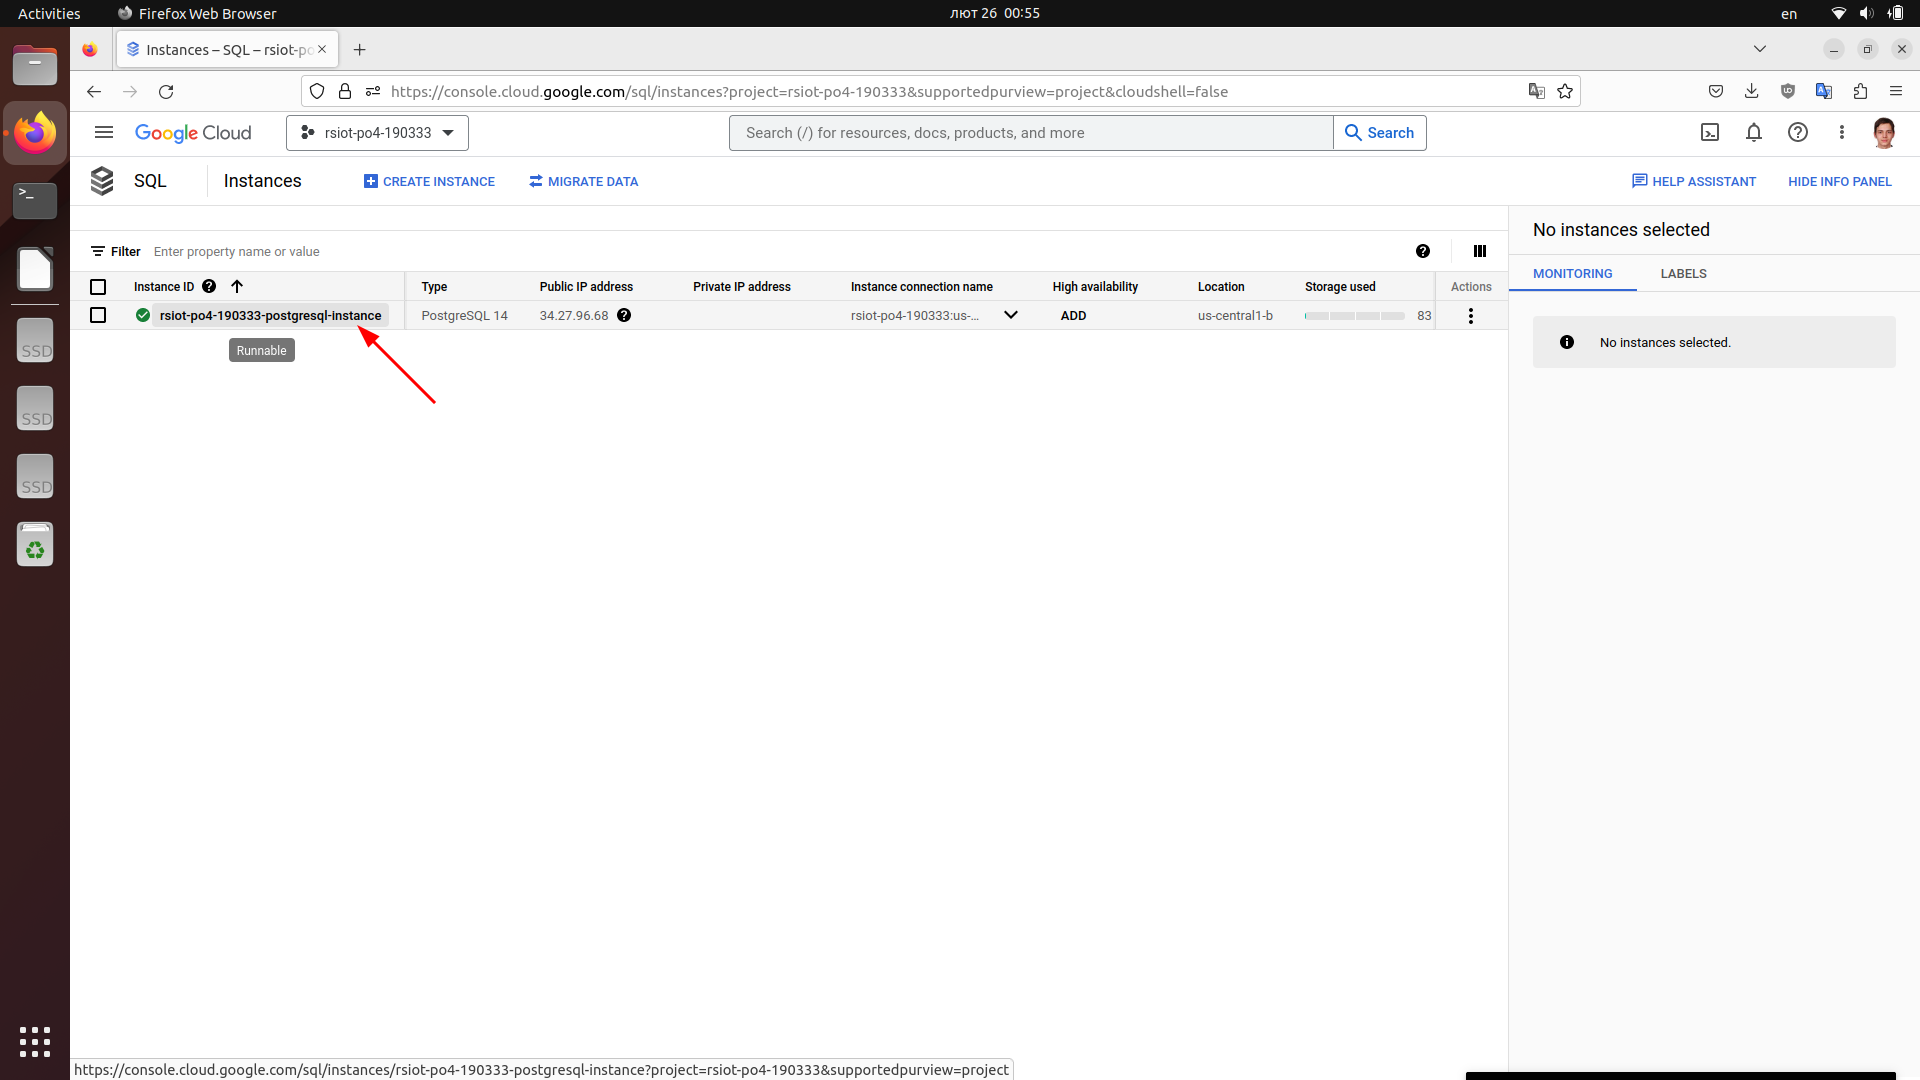
\includegraphics[width=10cm]
    {images/2023-02-26_00-55-24.png}
    \caption{\_}
    \label{fig:28}
  \end{figure}

  Жмём <<Databases>>. Жмём <<CREATE DATABASE>> (см. рисунок~\ref{fig:29}).

  Database Name: \underline{database}. Жмём <<CREATE>> (см. рисунок~\ref{fig:29}).

  \begin{figure}[!h]
    \centering
    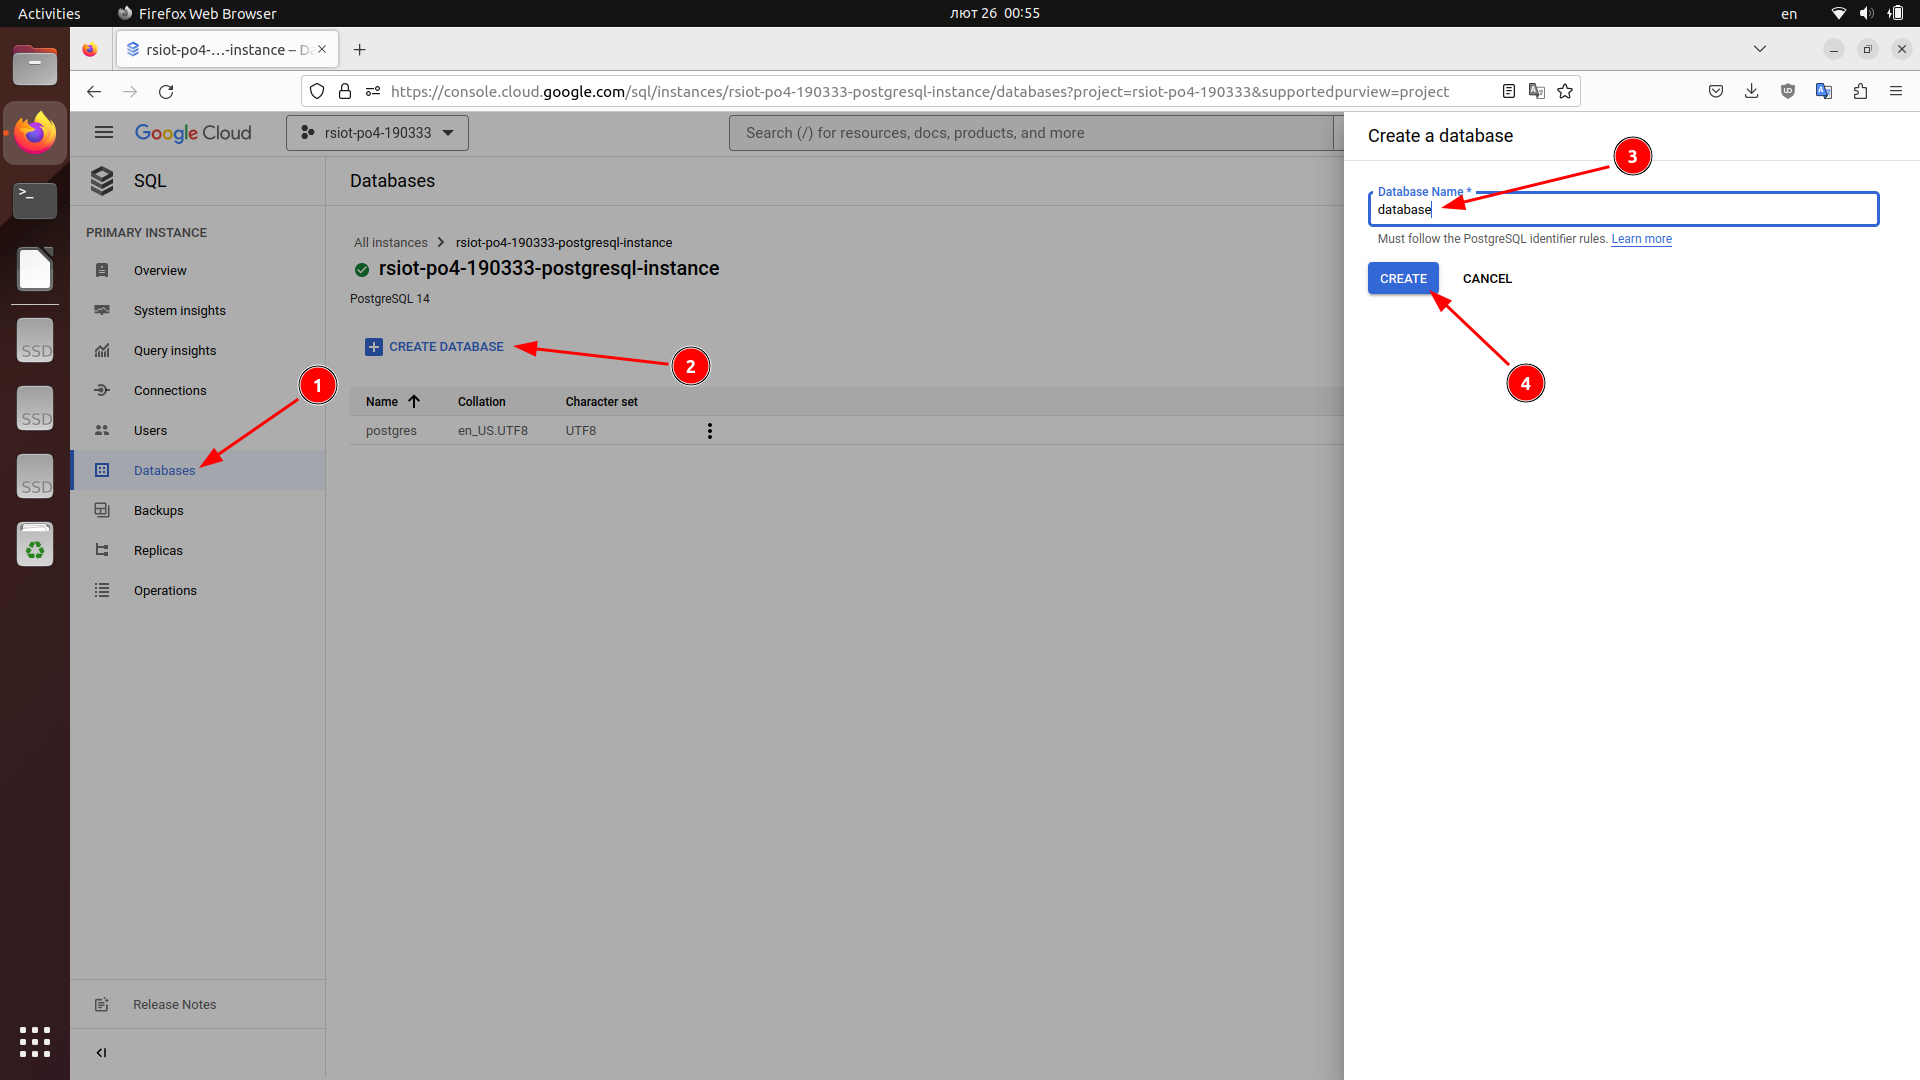
\includegraphics[width=10cm]
    {images/2023-02-26_00-56-11.png}
    \caption{\_}
    \label{fig:29}
  \end{figure}

  Жмём <<Users>>. Жмём <<ADD USER ACCOUNT>> (см. рисунок~\ref{fig:30}).

  User name: \underline{admin}. Password: \underline{secret123password}. Жмём <<ADD>> (см. рисунок~\ref{fig:30}).

  \begin{figure}[!h]
    \centering
    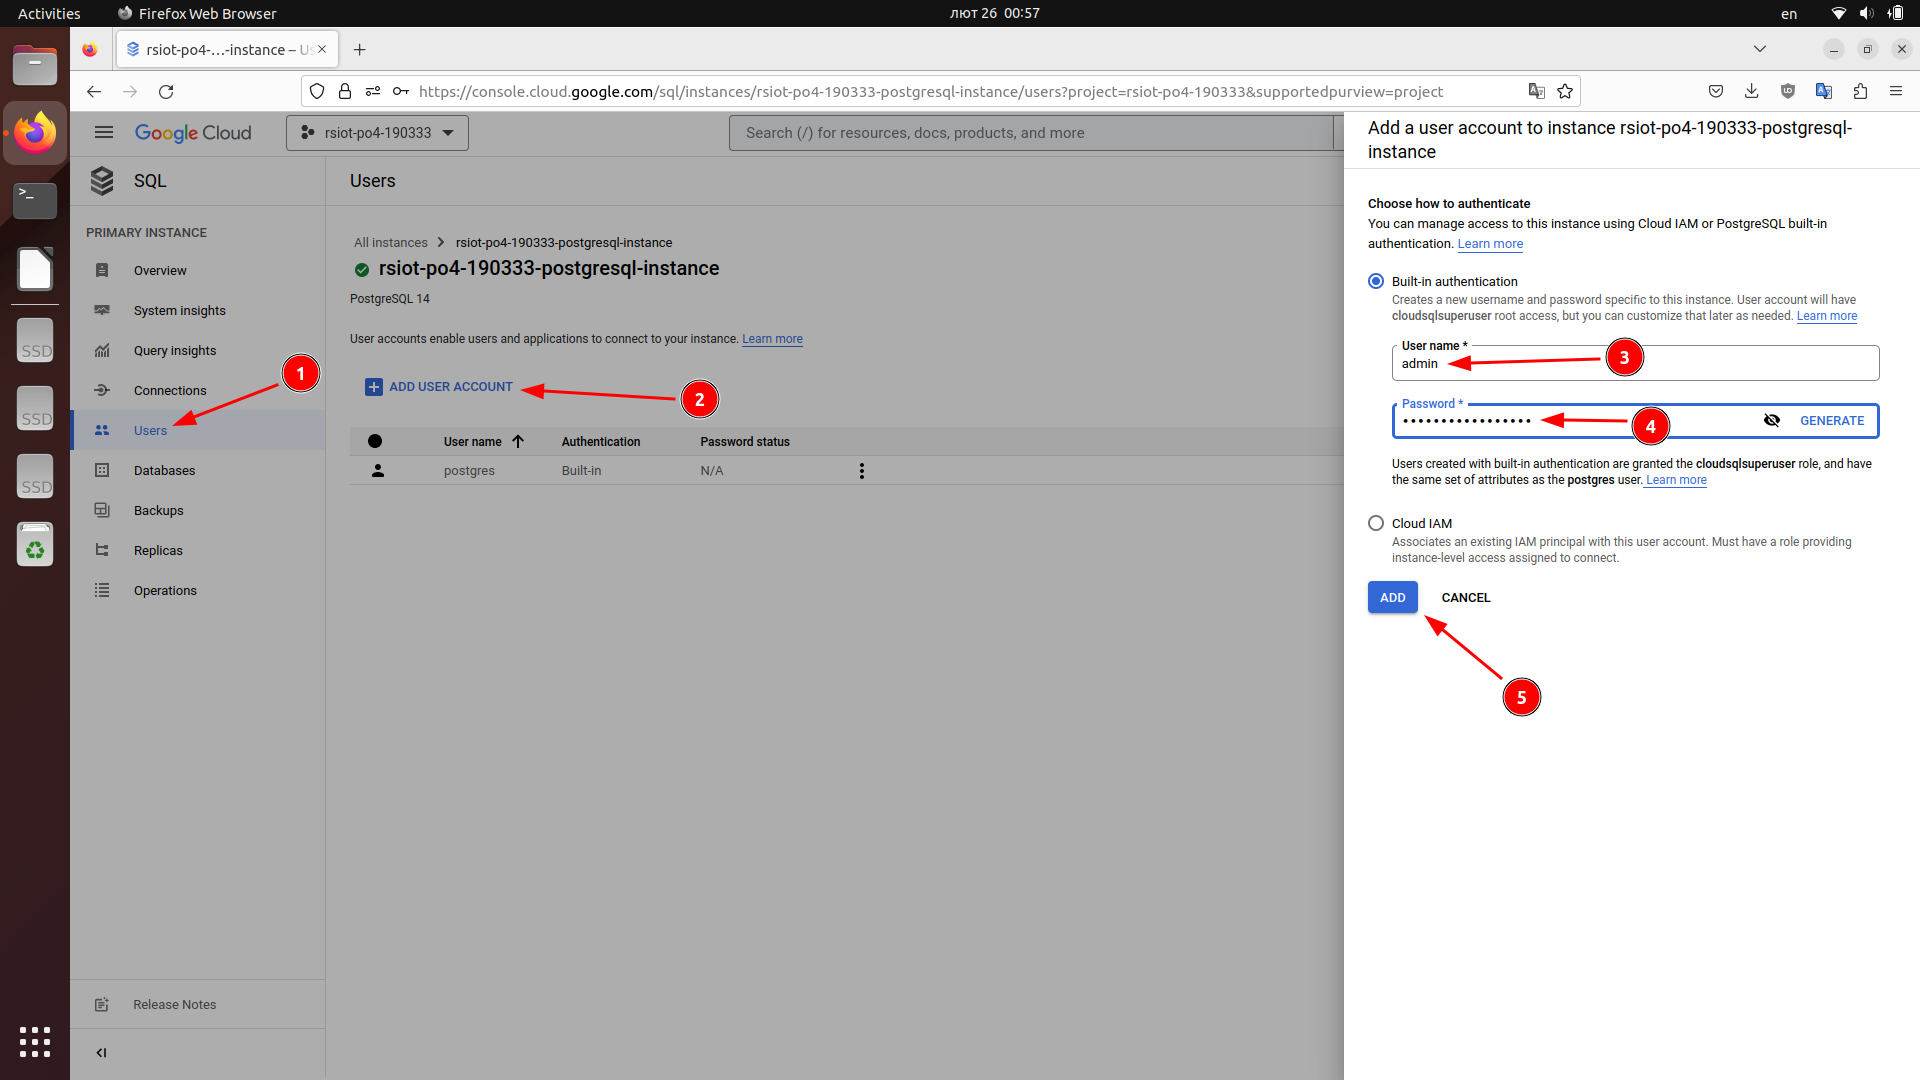
\includegraphics[width=11cm]
    {images/2023-02-26_00-57-31.png}
    \caption{\_}
    \label{fig:30}
  \end{figure}

  \newpage
  Заходим на сайт Google Cloud SQL \cite{GoogleCloudSql} (см. рисунок~\ref{fig:31}).

  \begin{lstlisting}[language=bash,name=Подключаюсь к БД через Google Cloud Shell]
    gcloud sql connect rsiot-po4-190333-postgresql-instance
    exit

    psql "host=<public-ip-address-google-cloud-sql> dbname=database user=admin"
  \end{lstlisting}

  \begin{lstlisting}[language=bash,name=Устанавливаю gcloud на ноутбук]
    mkdir ~/ph_apps -p

    mkdir ~/ph_apps/google-cloud-sdk -p

    cd ~/ph_apps/google-cloud-sdk

    curl -O https://dl.google.com/dl/cloudsdk/channels/
    rapid/downloads/google-cloud-cli-416.0.0-linux-x86_64.tar.gz

    tar -xf google-cloud-cli-416.0.0-linux-x86_64.tar.gz

    ./google-cloud-sdk/install.sh
    # n
    # y
    # Enter

    export PATH="$PATH:~/ph_apps/google-cloud-sdk/google-cloud-sdk/bin"

    sudo reboot
  \end{lstlisting}

  \begin{lstlisting}[language=bash,name=Подключаюсь к БД через ноутбук]
    gcloud projects list
    gcloud config set project rsiot-po4-190333
    gcloud sql connect rsiot-po4-190333-postgresql-instance
    exit

    psql "host=<public-ip-address-google-cloud-sql> dbname=database user=admin"
  \end{lstlisting}

  \begin{figure}[!h]
    \centering
    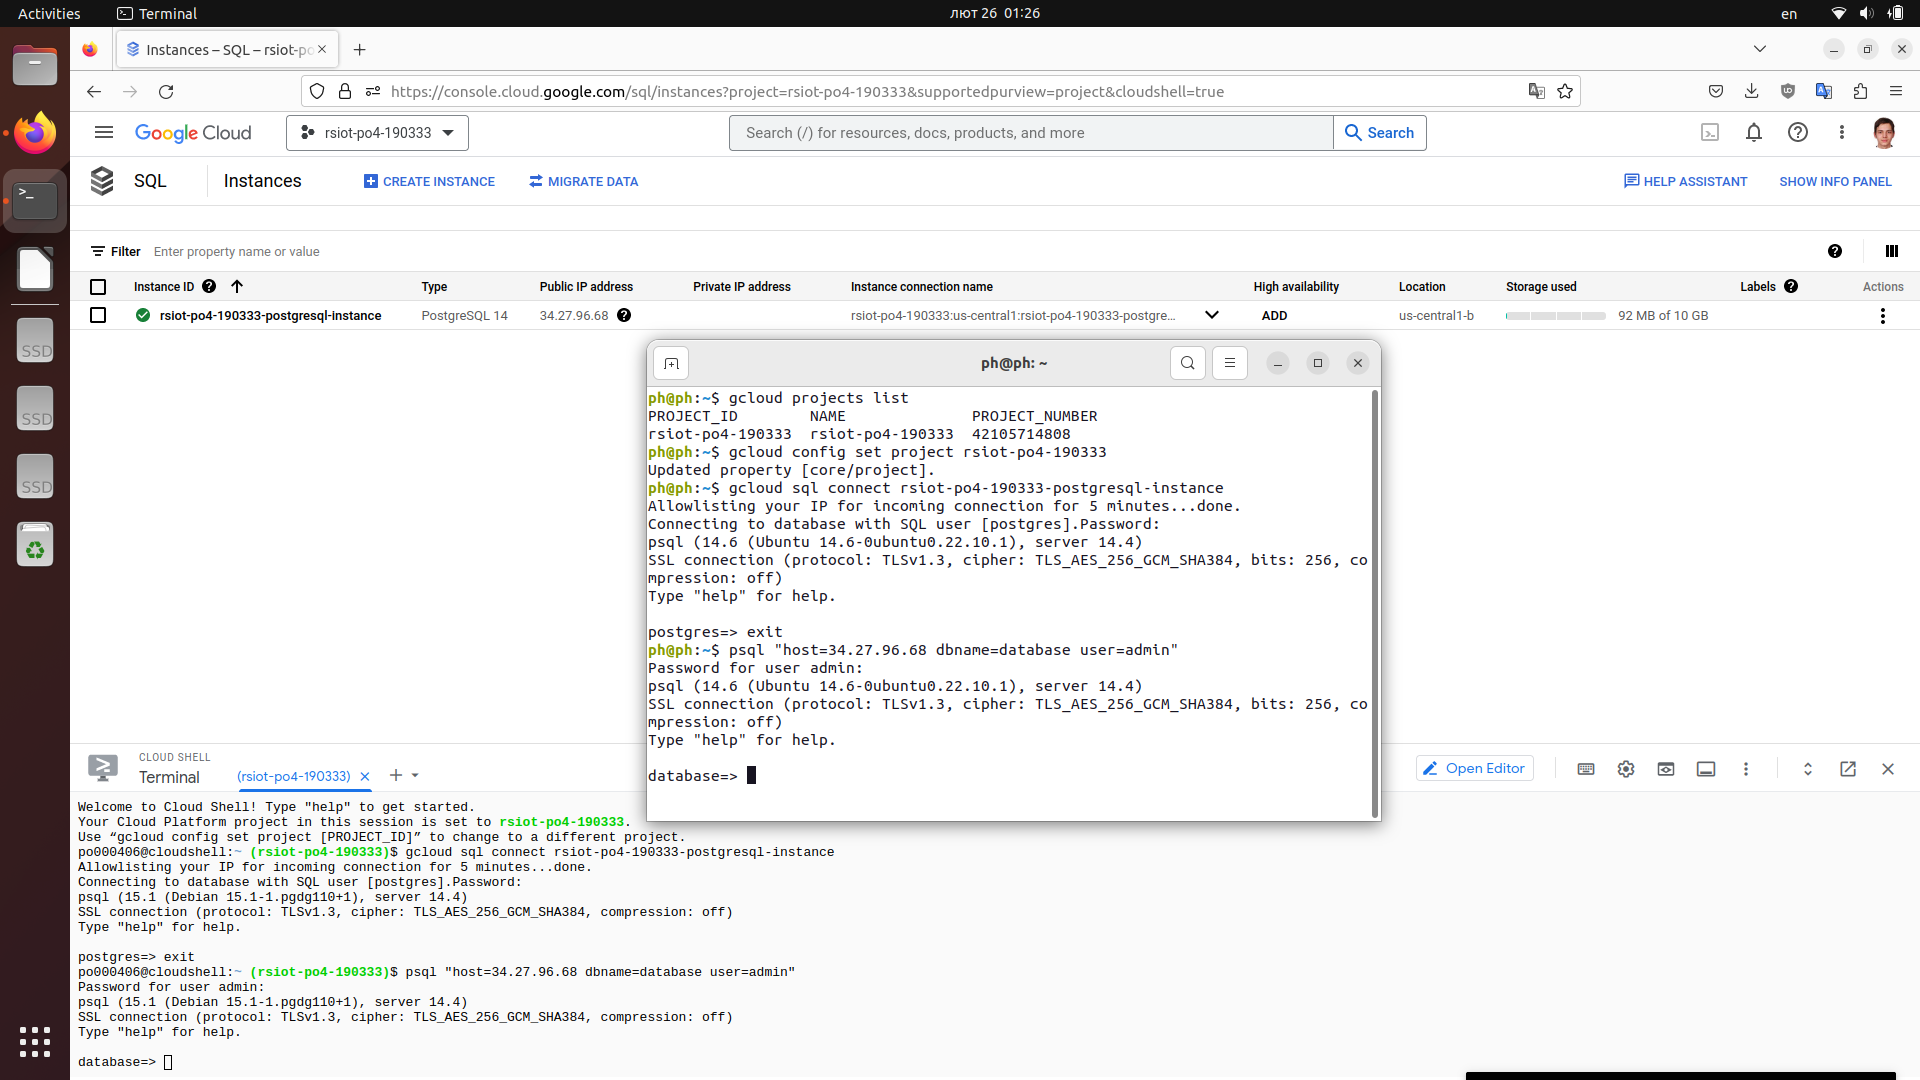
\includegraphics[width=11cm]
    {images/2023-02-26_01-26-15.png}
    \caption{\_}
    \label{fig:31}
  \end{figure}

  \newpage
  \textbf{Открываем логи Google Cloud Logs}

  Заходим на сайт Google Cloud Console \cite{GoogleCloudConsole} (см. рисунок~\ref{fig:32}).

  Menu > Logging > Logs Explorer \cite{GoogleCloudLogs} (см. рисунок~\ref{fig:32}).

  \begin{figure}[!h]
    \centering
    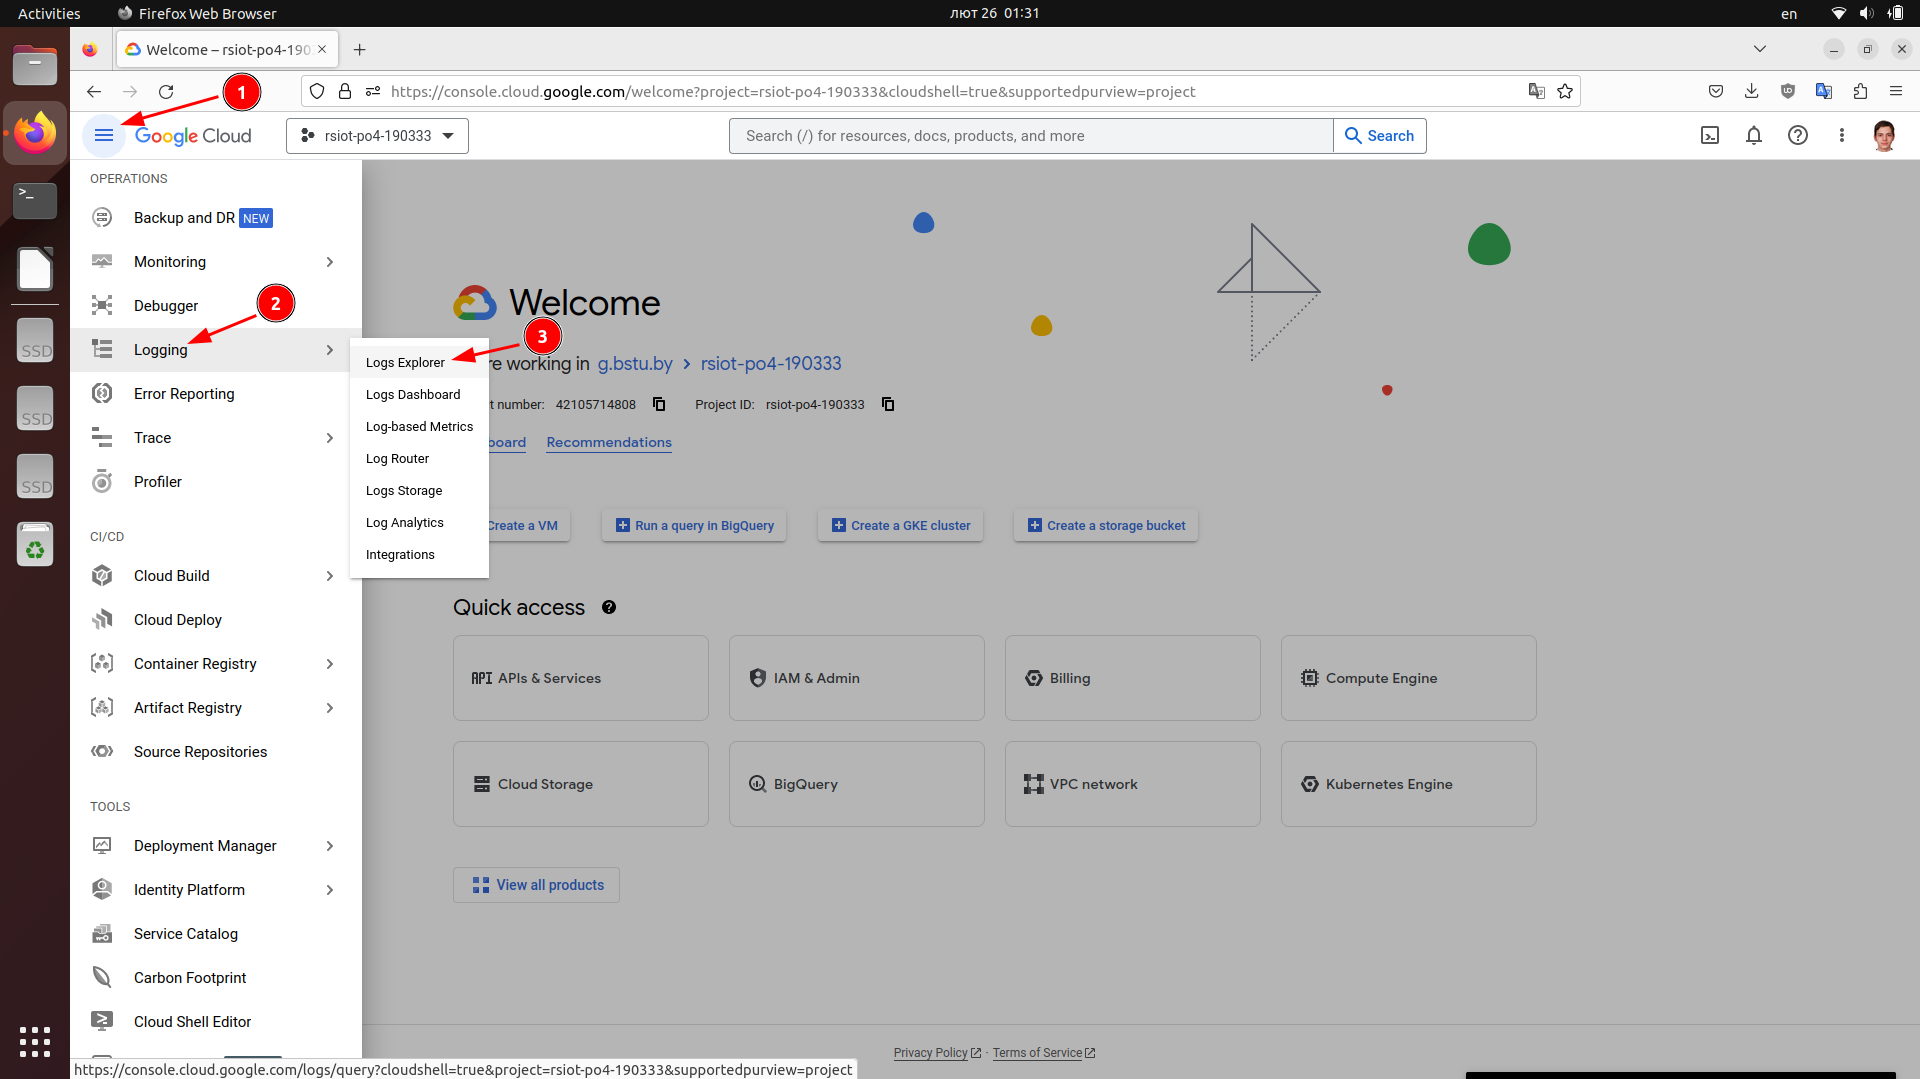
\includegraphics[width=14cm]
    {images/2023-02-26_01-32-00.png}
    \caption{\_}
    \label{fig:32}
  \end{figure}

  Жмём Just to now (см. рисунок~\ref{fig:33}).

  В этих логах удобно будет следить за выводами консоль MS3 запушеного в App Engine, которая будет в лабораторной работе номер 3.

  \begin{figure}[!h]
    \centering
    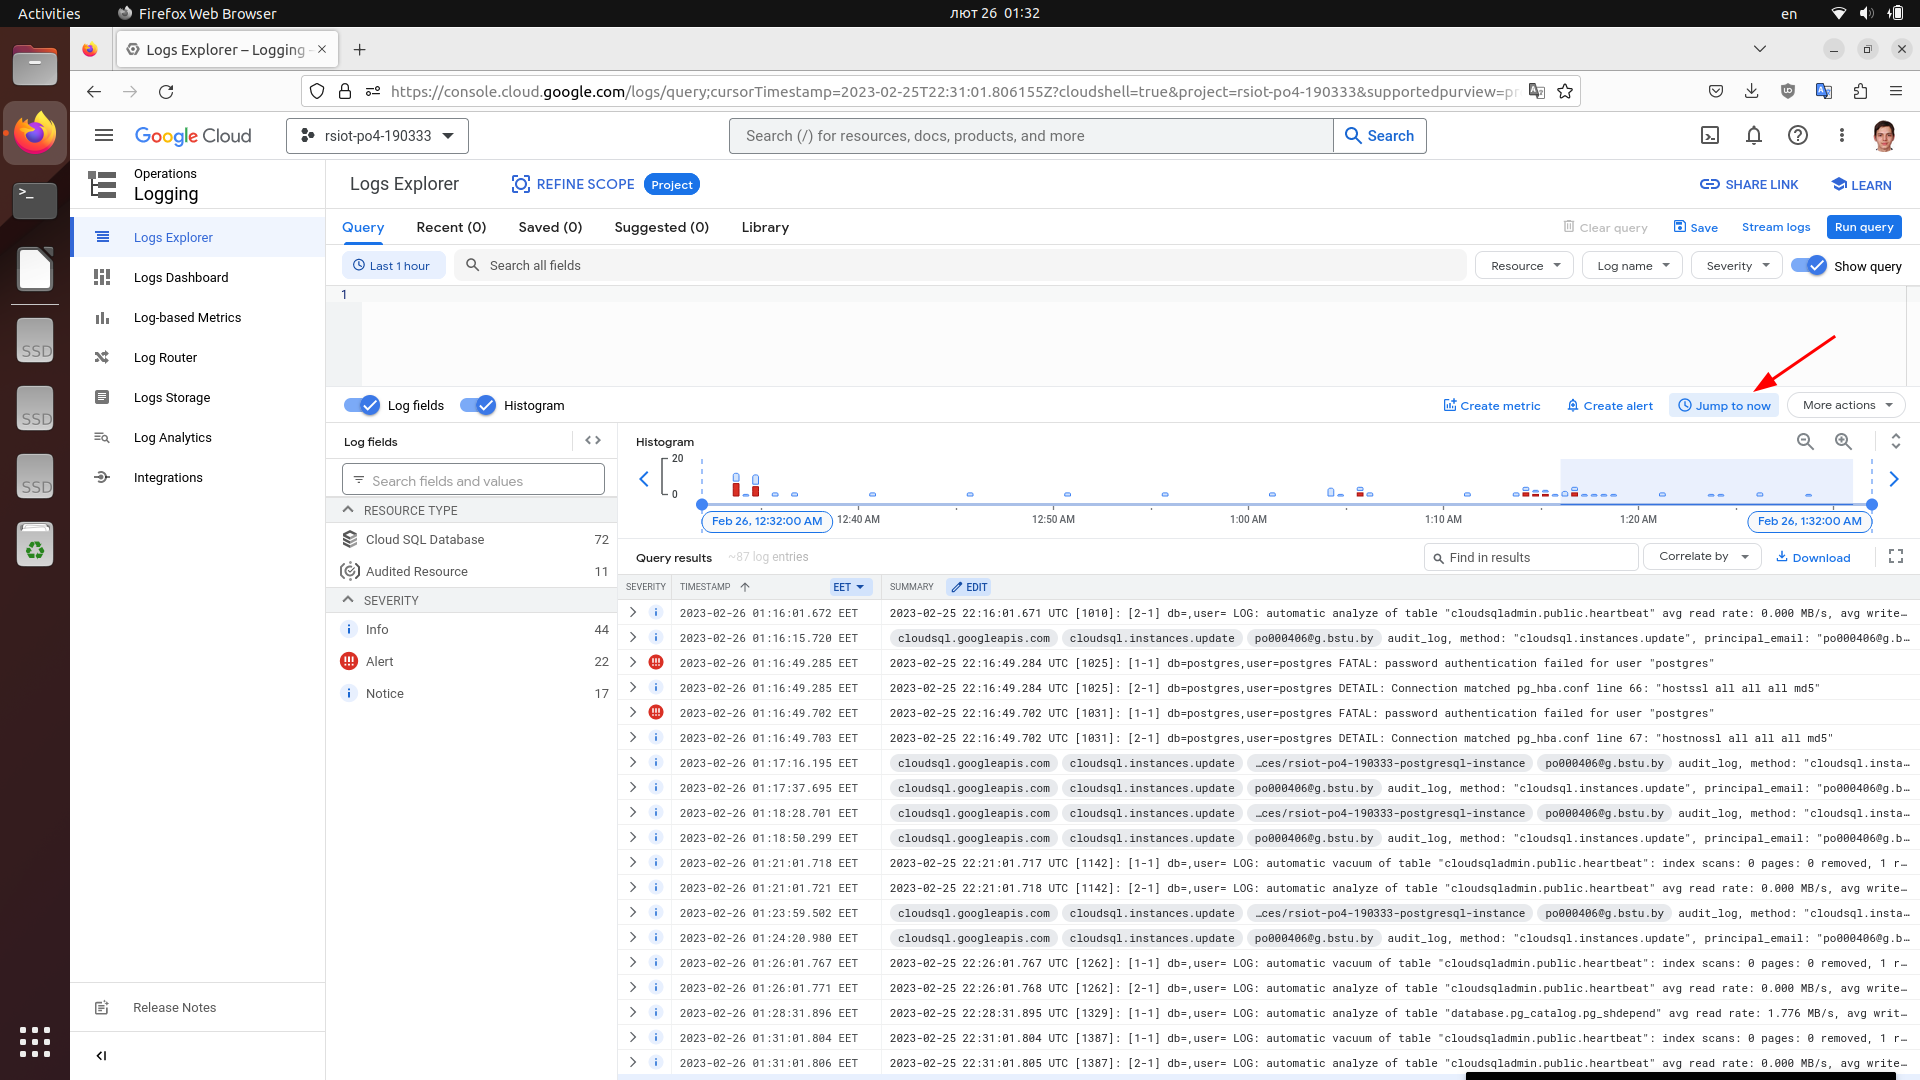
\includegraphics[width=16cm]
    {images/2023-02-26_01-32-59.png}
    \caption{\_}
    \label{fig:33}
  \end{figure}
  
  \paragraph{} \textbf{Вывод}:
  Создали Compute Engine. Сгенерировали приватный и публичный ключ. Добавили публичный ключ в настройки Compute Engine.
  Подключились по SSH к Compute Engine. Установили приложение и БД. Запустили приложение. Открыли порты.

  % = = = = = = = = = = = = = = = =
  \newpage
  \begingroup
    \phantomsection
    \addcontentsline{toc}{section}{СПИСОК ИСПОЛЬЗОВАННЫХ ИСТОЧНИКОВ}
    \section*{Список использованных источников} %\section*{СПИСОК ИСПОЛЬЗОВАННЫХ ИСТОЧНИКОВ}

    \renewcommand{\addcontentsline}[3]{}% Remove functionality of \addcontentsline
    \renewcommand{\section}[2]{}% Remove functionality of \section

    \begin{thebibliography}{}

    \bibitem{GoogleCloudConsole}
    Welcome – Google Cloud console
    [Electronic resource]. -
    Mode of access:
    \url{https://console.cloud.google.com/welcome}.
    Date of access: 26.02.2023.

    \bibitem{GoogleCloudComputeEngine}
    VM instances – Compute Engine – Google Cloud console
    [Electronic resource]. -
    Mode of access:
    \url{https://console.cloud.google.com/compute/instances}.
    Date of access: 26.02.2023.

    \bibitem{GoogleCloudFirewall}
    Firewall – VPC network – Google Cloud console
    [Electronic resource]. -
    Mode of access:
    \url{https://console.cloud.google.com/networking/firewalls/list}.
    Date of access: 26.02.2023.

    \bibitem{GoogleCloudSql}
    Instances – SQL – Google Cloud console
    [Electronic resource]. -
    Mode of access:
    \url{https://console.cloud.google.com/sql/instances}.
    Date of access: 26.02.2023.

    \bibitem{GoogleCloudLogs}
    Logs Explorer – Logging – Google Cloud console
    [Electronic resource]. -
    Mode of access:
    \url{https://console.cloud.google.com/logs/query}.
    Date of access: 26.02.2023.

  \end{thebibliography}
  \endgroup
  % = = = = = = = = = = = = = = = =
\end{document}
